%Documento principal do latex para uso no TCC da Univás.

\documentclass[a4paper, 12pt, chapter=TITLE, oneside, english, brazil]{abntex2}

\usepackage{styles/CodeStyle}      %Formatação de códigos e listagens
\usepackage{styles/EventFlowStyle} %Estilo para o quadro de fluxo de eventos
\usepackage{styles/NuapaStyle}     %Estilo exigido pela Univás

%Início do documento
\begin{document}

\pretextual %Início dos Elementos Pré-Textuais


\makeatletter
\renewcommand{\imprimircapa}{%
\begin{capa}%
\begin{center}%
  {\ABNTEXchapterfont\large\MakeUppercase\imprimirautor}\\
  \vspace*{\fill}%
  \vspace*{\fill}%
  \vspace*{\fill}%
  {\ABNTEXchapterfont\bfseries\Large\MakeUppercase\imprimirtitulo}\\
  \vspace*{\fill}%
  {\color{white}%
\abntex@ifnotempty{\imprimirpreambulo}{%
  \hspace{.45\textwidth}
  \begin{minipage}{.5\textwidth}
    \SingleSpacing
    \imprimirpreambulo
  \vspace{.1\textwidth}\\%
  {\imprimirorientadorRotulo:~\imprimirorientador}
  \abntex@ifnotempty{\imprimircoorientador}{%
    \hspace{.45\textwidth}
    {\large\imprimircoorientadorRotulo~\imprimircoorientador}%
  }%
  \end{minipage}%
}%
\color{black}}%
  \vspace*{\fill}\\%
  {\ABNTEXchapterfont\large\bfseries\MakeUppercase\imprimirinstituicao}\\
  {\large\bfseries\MakeUppercase\imprimirlocal}\\
  {\large\bfseries\MakeUppercase\imprimirdata}
\end{center}
\end{capa}
}
\makeatother

\imprimircapa

%% folha de rosto 
%\folhaderostoname{Folha de rosto}
%http://code.google.com/p/abntex2/wiki/ComoCustomizar

\makeatletter
\renewcommand{\folhaderostocontent}{
\begin{center}%
  {\ABNTEXchapterfont\large\MakeUppercase\imprimirautor}\\
  \vspace*{\fill}%
  \vspace*{\fill}%
  \vspace*{\fill}%
  {\ABNTEXchapterfont\bfseries\Large\MakeUppercase\imprimirtitulo}\\
  \vspace*{\fill}%
\abntex@ifnotempty{\imprimirpreambulo}{%
  \hspace{.45\textwidth}
  \begin{minipage}{.5\textwidth}
    \SingleSpacing
    \imprimirpreambulo
  \vspace{.1\textwidth}\\%
  {\imprimirorientadorRotulo:~\imprimirorientador}
  \abntex@ifnotempty{\imprimircoorientador}{%
    \hspace{.45\textwidth}
    {\large\imprimircoorientadorRotulo~:\imprimircoorientador}%
  }%
  \end{minipage}%
}%
  \vspace*{\fill}\\%
  {\ABNTEXchapterfont\large\bfseries\MakeUppercase\imprimirinstituicao}\\
  {\large\bfseries\MakeUppercase\imprimirlocal}\\
  {\large\bfseries\MakeUppercase\imprimirdata}
\end{center}
}%end of folhaderostocontent
\makeatother

\imprimirfolhaderosto*{}
%\begin{fichacatalografica}
\begin{normalsize}
  \vspace*{\fill}
  % Posição vertical
%  \hrule
  % Linha horizontal
  \begin{center}
  \fbox{
    % Minipage Centralizado
    \begin{minipage}[c]{12.5cm} % Largura
      \vspace{0.7cm}%
      \hspace{0.8cm} \imprimirAutorCitacao ~\\%
      
      \hspace{0.8cm} \imprimirtitulo ~/ \imprimirAutorUm , \imprimirAutorDois ~-- \imprimirlocal: Univás, \imprimirdata. %
      
     %\hspace{0.8cm} \pageref{LastPage} f. : il.~\\%
	  \hspace{0.8cm} 100 f. : il.~\\%
      
      \hspace{0.8cm} \imprimirtipotrabalho~--~\imprimirinstituicao , Univás, \imprimircurso. % 
      
      \hspace{0.8cm} \imprimirorientadorRotulo: ~\imprimirorientador ~\\%

      \hspace{0.8cm} 1. \imprimirPalavraChaveUm. 2. \imprimirPalavraChaveDois. 3. \imprimirPalavraChaveTres. ~ \\%
    \end{minipage}
    }
  \end{center}
\end{normalsize}
\end{fichacatalografica}
\newpage
%\setlength{\ABNTEXsignwidth}{10cm}

\begin{folhadeaprovacao}
  \begin{center}
    {\ABNTEXchapterfont\large\MakeUppercase\imprimirautor}
    \vspace*{\fill}
    \vspace*{\fill}
    \vspace*{\fill}
    \par
    {\ABNTEXchapterfont\bfseries\Large\MakeUppercase\imprimirtitulo}
    \vspace*{\fill}
  \end{center}
  Trabalho de conclusão de curso defendido e aprovado em \imprimirDataDaAprovacao ~pela banca examinadora constituída pelos professores:

  ~\newline
  \begin{flushleft}
  \assinatura*{\imprimirorientador \\ \imprimirorientadorRotulo }
  \assinatura*{\imprimirAvaliadorUm \\ \imprimirAvaliadorLabelUm }
  \assinatura*{\imprimirAvaliadorDois \\ \imprimirAvaliadorLabelDois}
  \end{flushleft}
  \vspace*{\fill}
  \vspace*{\fill}
\end{folhadeaprovacao}

%\begin{dedicatoria}
\vspace*{\fill}
\vspace*{\fill}
\vspace*{\fill}
\vspace*{\fill}
\vspace*{\fill}
\vspace*{\fill}
De \imprimirAutorUm.
\newline
%início da dedicatória do autor um
Dedico este trabalho \ldots 

\vspace*{\fill}
De \imprimirAutorDois.
\newline
%início da dedicatória do autor dois
Dedico este trabalho \ldots

\end{dedicatoria}

%\begin{agradecimentos}

De \imprimirAutorUm
\newline
%início do agradecimento do autor um
\par Agradeço \ldots

\vspace*{\fill}
De \imprimirAutorDois
\newline
%início do agradecimento do autor dois
\par Agradeço \ldots

\end{agradecimentos}





%\begin{epigrafe}
\vspace*{\fill}
\begin{flushright}
\textit{‘‘e não vos conformeis com este mundo, mas transformai-vos pela renovação da vossa mente, para que proveis qual é a boa, agradável e perfeita vontade de Deus.\\
(Romanos 12:2)}
\end{flushright}
\end{epigrafe}

%% --- resumo em português ---

\begin{OnehalfSpacing} 

\noindent \imprimirAutorCitacaoMaiuscula. {\bfseries\imprimirtitulo}. {\imprimirdata}.  Monografia -- Curso de {\MakeUppercase\imprimircurso}, {\imprimirinstituicao}, {\imprimirlocal}, {\imprimirdata}.

\vspace{\onelineskip}
\vspace{\onelineskip}
\vspace{\onelineskip}
\vspace{\onelineskip}

\begin{resumo}
~\\
%início do texto do resumo
\noindent Os algoritmos genéticos, inspirados na genética e na teoria da evolução das espécies de Charles Darwin,
são algoritmos probabilísticos que, aleatoriamente, promovem uma busca paralela pela melhor solução de um problema e são 
desenvolvidos baseados no princípio de sobrevivência dos mais aptos, na reprodução e na mutação dos indivíduos, de forma a fazer com 
que soluções evoluam e se tornem cada vez melhores. A presente pesquisa apresenta uma visão geral sobre
o conceito de algoritmos genéticos, demonstrando seus fundamentos, operadores e suas configurações, realizando um comparativo 
com os conceitos semelhantes na natureza. Para ilustrar a utilização desta técnica, foi desenvolvida uma aplicação, 
em plataforma WEB, juntamente com um algoritmo genético, que visa encontrar soluções otimizadas para distribuição 
das atividades de um sistema de produção de calças de modo que permita aos empregados trabalharem em suas 
casas e que cada parte da calça seja confeccionada separadamente. O software recebe, como entrada, dados de tempo e preço
de produção por peça de cada empregado e, após a execução do algoritmo genético sobre estes dados, apresenta como saída uma 
boa forma de distribuição das atividades que permita que a produção seja realizada com o menor tempo e tenha o menor custo possível 
dentro do prazo de entrega. Esta pesquisa é do tipo aplicada, pois não visa modificar os processos de produção e sim apresentar 
formas de otimizá-los.

%fim do texto do resumo
\vspace{\onelineskip}
\vspace*{\fill}
\noindent \textbf{Palavras-chave}: \imprimirPalavraChaveUm. \imprimirPalavraChaveDois. \imprimirPalavraChaveTres. \imprimirPalavraChaveQuatro.
\vspace{\onelineskip}
\end{resumo}

\end{OnehalfSpacing}

%% --- resumo em inglês ---

\begin{OnehalfSpacing} 

\noindent \imprimirAutorCitacaoMaiuscula. {\bfseries\imprimirtitulo}. {\imprimirdata}.  Monografia -- Curso de {\MakeUppercase\imprimircurso}, {\imprimirinstituicao}, {\imprimirlocal}, {\imprimirdata}.

\vspace{\onelineskip}
\vspace{\onelineskip}
\vspace{\onelineskip}
\vspace{\onelineskip}

\begin{resumo}[Abstract]%
\begin{otherlanguage*}{english}%
\textit{
%início do texto do abstract
\noindent This work presents \ldots
%fim do texto do abstract
}

\vspace{\onelineskip}
\vspace*{\fill}
\noindent \textbf{Key words}: \imprimirKeyWordOne. \imprimirKeyWordTwo. \imprimirKeyWordThree.
\end{otherlanguage*}
\vspace{\onelineskip}
\end{resumo}

\end{OnehalfSpacing}

%%Lista de Figuras
\pdfbookmark[0]{\listfigurename}{lof}
\listoffigures*
\cleardoublepage

% Lista de Quadros
\pdfbookmark[0]{\listofquadrosname}{loq}
\listofquadros*
\cleardoublepage

%Lista de Tabelas
\pdfbookmark[0]{\listtablename}{lot}
\listoftables*
\cleardoublepage

%Lista de Códigos
\counterwithout{lstlisting}{chapter}
\pdfbookmark[0]{\lstlistingname}{lol}
%http://tex.stackexchange.com/questions/50031/how-to-remove-contents-line-from-table-of-contents
\begin{KeepFromToc}
\lstlistoflistings
\end{KeepFromToc}
\cleardoublepage

%%Lista de siglas
%ver http://marc.info/?l=tex-br&m=110566665520790 para colocar em ordem alfabética.

\begin{SingleSpace}

\begin{siglas}
\item[ABNT] Associação Brasileira de Normas Técnicas
\item[API] \textit{Application Programming Interface}
\item[GNU] \textit{Gnu is Not Unix}
\item[GPL] \textit{General Public License}
\item[MVC] \textit{Model -- View -- Controller}
\end{siglas}

\end{SingleSpace}

%%Sumário
%ver esse link para configuração de fonte: http://tex.stackexchange.com/questions/83377/how-to-change-chapter-font-style-in-the-middle-of-the-table-of-the-contents
\pdfbookmark[0]{\contentsname}{toc}
\begin{SingleSpace} 
\tableofcontents*
\end{SingleSpace}
\cleardoublepage


\textual %Início dos Elementos Textuais

%%\chapter*{Introdução}
\begin{center}
  \vspace{1.2em}
  \textbf{\large INTRODUÇÃO}
  \vspace{2.9em}
\end{center}
\thispagestyle{empty}

\addcontentsline{toc}{chapter}{INTRODUÇÃO}
\stepcounter{chapter} %incrementa o número do capítulo

%\par Exemplo simples de parágrafo utilizando o comando\texttt{$\backslash$par}.
% Pode-se utilizar (in\-cons\-titucional (exemplo de forçar separação de sílabas)).

\par Sabe-se   que   atualmente   existem   diversos   softwares  
disponíveis no mercado.   Programas que   vão   desde   aqueles   desenvolvidos   sob   medida
até   softwares   genéricos   popularmente chamados   de   “softwares   de   prateleira”.
Porém   no   cenário   corporativo,   levando   em   consideração que   empresas   buscam
a   cada   dia   se   tornarem   mais   competitivas,   é   necessário   que   um   sistema  
ofereça   suporte   para   que   estas   possam   se tornar   mais   eficientes,
como   por exemplo,   auxiliar   na  busca   pela   diminuição   dos   custos   operacionais   para   que
assim   seja   possível   alcançar   os   melhores  preços de venda. \cite{livro_laudon_sistemas_de_informacoes_gerenciais} 

\par Neste   contexto,   a   ideia   de   agregar   características  
semelhantes  à inteligência   humana   aos programas se torna uma alternativa
interessante, pois segundo
\citeonline[p.329]{livro_laudon_sistemas_de_informacoes_gerenciais},

\begin{citacao}
Técnicas inteligentes ajudam os tomadores de decisão capturando o
conhecimento coletivo e individual, descobrindo padrões e  comportamentos
em grande quantidade de dados e gerando   soluções para problemas  amplos
e   complexos   demais   para   serem resolvidos por seres humanos.
\end{citacao} 

\par O conceito por trás deste pensamento é denominado Inteligência Artificial -
IA\footnotemark[1] - e é definido por \citeonline{artificial_intelligence}, como
uma área da ciência da computação que abrange a automatização da inteligência.

\par Para \citeonline[p.44]{ags_java_magazine}, “a IA é inspirada  em  
processos naturais e está relacionada à reprodução de   capacidades  
normalmente   associadas   à   inteligência   humana,   como aprendizagem,
adaptação,   o   raciocínio,   entre   outras”.   Ainda   segundo   os   mesmos
autores,   várias  abordagens   surgiram   ao   longo   da   história   tais   como  
a abordagem   conexionista,   inspirada   nos  neurônios   biológicos,   a  
simbolista, baseada   na   inferência   humana   e   a   evolutiva, fundamentada na teoria
de evolução das espécies.

\par Na busca por otimizar seu processo de produção, uma empresa da região, que
fabrica calças e aloca costureiras que trabalham em suas casas, deseja saber
qual a melhor forma de distribuir o trabalho para que um determinado lote de seu produto
seja produzido no menor tempo possível e com o menor custo. Para a resolução
deste problema, pode se fazer uso de IA através de um dos ramos da abordagem
evolutiva denominado Algoritmos Genéticos - AGs\footnotemark[2] - pois, como
afirma \citeonline{nocoes_geriais_anita_fernandes}, os AGs resolvem problemas de
otimização através de um processo que oferece como saída a melhor solução
dentro de várias possíveis formas de se resolver um problema.

\footnotetext[1]{O termo Inteligência Artificial será referenciado pela sigla IA
a partir deste ponto do trabalho.}

\footnotetext[2]{O termo Algoritmos Genéticos será referenciado pela sigla AGs
a partir deste ponto do trabalho.}

\par O presente trabalho têm por objetivo geral, desenvolver uma aplicação
utilizando técnicas de inteligência artificial, capazes de realizar a alocação
de empregados em uma linha de produção de forma otimizada. Para a realização do mesmo foram
colocados os seguintes objetivos específicos: a) Demonstrar o uso de algoritmos
genéticos; b) Projetar uma aplicação em plataforma WEB que distribua as
atividades de uma linha de produção de calças de forma inteligente, a fim de se
obter o menor custo e o menor tempo de produção.

\par Para \citeonline {livro_ags_ricardo_linden}, AGs é definido
como uma técnica de otimização e busca que se baseia na teoria do processo de evolução e seleção
natural, proposto por Charles Darwin em seu livro A Origem das Espécies, que
afirma que indivíduos com melhor capacidade de adaptação ao seu ambiente possuem
maior chance de sobreviver e gerar descendentes.

\par Segundo \citeonline {nocoes_geriais_anita_fernandes}, o termo foi proposto
por Holland, em 1975, e por imitação à teoria da evolução, é representado por
uma população de indivíduos que representam soluções para um determinado problema e então tais soluções
podem evoluir até se chegar a uma solução ótima.

\par Vários trabalhos foram desenvolvidos utilizando a robustez de AGs, dentre
eles o trabalho de \citeonline{santos2007seleccao}, que faz a seleção de
atributos usando AGs para classificação de
regiões, o trabalho de \citeonline{silva2001otimizaccao}, que descreve a
otimização de estruturas de concreto armado utilizando AGs e 
o trabalho de \citeonline{freitas2007ferramenta} que descreve uma ferramenta
baseada em AGs para a geração de tabela de horário escolar.

\par O sistema desenvolvido neste trabalho, assim como nos outros citados, 
tem o mesmo conceito, o de otimizar processos. No caso da fábrica de calças, 
tal otimização irá promover a diminuição do custo de produção das calças confeccionadas, 
permitindo assim com que estas possam ser vendidas também por um preço melhor, 
beneficiando assim, os consumidores da região. 
Além disso, a ideia de otimizar procedimentos, muitas vezes, também contribui
para a preservação de recursos naturais devido ao fato de que processos otimizados 
podem significar economia de energia e diminuição de emissão de gases. 
No caso da empresa de calças, se o gestor ter sempre em mãos a solução mais otimizada, 
irá ter um menor tempo de transporte de materiais, o que irá reduzir a emissão de gases 
dos veículos utilizados no transporte de materiais e peças entre as costureiras.

\par No âmbito acadêmico, o trabalho agregará à base de conhecimento
da Univás um material que faça referência a tecnologias e conceitos de inteligência
artificial, que hoje estão presentes em diversos sistemas críticos de apoio a
decisão e otimização de processos nas empresas.

%\par O \LaTeX~faz a ifenização automática, porém existem casos que é necessário
% forçá-lo. Veja no parágrafo anterior como forçar a ifenização, na palavra: inconstitucional.

%\par Existem várias formas de fazer referências. As duas formas mais comuns
% são: a primeira é assim: \cite{livro_laudon_sistemas_de_informacoes_gerenciais}, e a outra é mostrada conforme \cite{ecocentro}.


%
%\chapter{JUSTIFICATIVA}

\par A otimização de processos nas empresas promove a diminuição
de custos permitindo  com que estas possam vender seus produtos por um preço
melhor. Além disso, a ideia de otimizar procedimentos, muitas vezes, também
contribui para a preservação de recursos naturais devido ao fato de que processos otimizados
podem significar economia de energia e diminuição de emissão de gases. No
caso da empresa de calças, se o gestor ter sempre em mãos a solução mais
otimizada, irá ter um menor tempo de transporte de materiais, o que irá reduzir a emissão de gases
de seus veículos na natureza. Além disso, ele poderá vender as calças por um preço
melhor o que irá beneficiar os consumidores da região.

\par Isso justifica a criação de uma aplicação inteligente que, através de uma
gama de soluções para o planejamento da produção, encontre aquela que seja a
mais eficiente.

\par No âmbito acadêmico, o trabalho agregará à base de conhecimento da Univás
um material que faça referência a tecnologias e conceitos de inteligência
artificial, que hoje estão presentes em diversos sistemas críticos de apoio a
decisão e otimização de processos nas empresas.

%\chapter{OBJETIVOS}

\par Esta sessão apresenta os objetivos a serem alcançados com este projeto.

\section{Objetivo Geral}

\begin{itemize}

  Desenvolver uma aplicação, utilizando técnicas de inteligência artificial,
  capaz de  realizar a alocação de empregados em uma linha de produção de forma
  otimizada.
  
\end{itemize}

\section{Objetivos específicos}
  
 \begin{itemize}

	\item Demonstrar o uso de algoritmos genéticos;
	  
	\item Projetar uma aplicação em plataforma WEB que distribua as atividades de
	uma linha de produção de calças de forma inteligente, a fim de se obter o
	menor custo e o menor tempo de produção.
	
 \end{itemize}
  
\chapter{QUADRO TEÓRICO} \label{quadro_teorico}

\par Neste capítulo serão listados os conceitos e as tecnologias que serão
utilizados no desenvolvimento da proposta de trabalho apontada na seção 
objetivos. Para tal, serão discutidos a definição, o histórico e as 
aplicabilidades de cada um deles, tomando por base autores fundantes e 
seus comentaristas. É importante ressaltar que o texto desta seção, quando
descreve a teoria da evolução das espécies, não tem como objetivo levantar
questões sobre a origem dos seres vivos.

\section{Algoritmos Genéticos}

\par Nesta seção será descrito como surgiu, conceitos e algumas características
dos Algoritmos Genéticos, tema principal deste trabalho e fundamental para o
desenvolvimento da aplicação.

\subsection{Fundamentos}

\par Para \citeonline{livro_introduction_ag_melaine_mitchell}, desde o começo da
era computacional, cientistas pioneiros, tais como Alan Turing, John von
Neumann, Norbert Wiener e outros, tinham o objetivo de dotar os computadores de inteligência
de maneira que eles pudessem tomar decisões, se adaptar a determinadas situações
e até mesmo ter a capacidade de aprender. Com esta motivação, estes cientistas
se interessaram por outras áreas, além da eletrônica, como  a
biologia e a psicologia, e começaram então a realizar pesquisas para simular os
sistemas naturais no mundo computacional a fim de alcançarem suas metas. 

\par Vários conceitos computacionais baseados na natureza surgiram então ao
longo do tempo, dentre eles, a computação evolucionária inspirada na teoria da
evolução natural, da qual o exemplo mais proeminente são os AGs que foram
introduzidos por Jhon Holland, seu aluno David Goldberg e outros estudantes da universidade de Michigan.
\citeonline{livro_genetic_algorithm_goldberg} define os AGs como métodos de busca baseados na
genética e no mecanismo de seleção natural que permitem a possibilidade de obter
robustez e eficácia na tarefa de encontrar uma boa solução para um problema
em um espaço de busca complexo, em um tempo aceitável.


\par Segundo \citeonline{livro_ags_ricardo_linden}, a teoria da evolução foi proposta pelo naturalista
inglês Charles Darwin por volta de 1850, quando este, em uma viagem de navio
visitou vários lugares e por ser uma pessoa com uma grande habilidade de  observação, percebeu que indivíduos de uma mesma espécie vivendo em lugares diferentes possuíam também
características distintas, ou seja, cada indivíduo  possuía atributos
específicos que lhe permitia uma melhor adaptação em seu ecossistema. 


\par O autor afirma então que, com base nesta observação, Darwin propôs que existe um processo de
seleção natural, afirmando que, como os recursos na natureza, tais como água e comida,
são limitados, os indivíduos competem entre si e aqueles que não possuem atributos necessários
à adaptação ao seu ambiente tendem a ter uma probabilidade menor de reprodução e
irão ser extintos ao longo do tempo e, por outro lado, aqueles
com características que os permitem obter vantagens competitivas no meio onde
vivem, acabam tendo mais chances de sobreviver e gerar indivíduos ainda mais
adaptados. 

\par A teoria ressalta porém que o processo não tem o objetivo de maximizar
algumas características das espécies, pois  os novos indivíduos
possuem atributos que são resultados da mesclagem das características dos reprodutores,
o que faz com que os filhos não sejam exatamente iguais aos pais, podendo assim
ser superiores, uma vez que, estes herdem as qualidades de seus pais ou
inferiores se os descendentes herdarem as partes ruins de seus
reprodutores \cite{livro_ags_ricardo_linden}.

\par Para entender a relação entre AGs e a evolução natural é
necessário conhecer as principais terminologias biológicas, 
sendo importante ressaltar porém que, de acordo com
\citeonline{livro_introduction_ag_melaine_mitchell}, apesar da 
analogia a certos termos da biologia, a forma com que os AGs 
são implementados é relativamente simples se comparado ao funcionamento
biológico real.

\par \citeonline{livro_introduction_ag_melaine_mitchell} afirma que 
todos os seres vivos são compostos de células e estas possuem um ou mais
cromossomos que, basicamente, são manuais de instruções que definem as 
características do organismo. O cromossomo é formado por um conjunto de genes
que, em grupo ou individualmente, são responsáveis por um determinado atributo
do indivíduo como por exemplo, a cor do cabelo, a altura, etc. Cada gene possui
uma localização dentro do cromossomo denominada \textit{locus} e, por fim, o
conjunto de todos os cromossomos dentro da célula é definido como genoma. 

\par Considerando isto, \citeonline[p.33]{livro_ags_ricardo_linden} afirma que,

\begin{citacao}
	Um conjunto específico de genes no genoma é chamado de genótipo. O
	genótipo é a base do fenótipo, que é a expressão das características
	físicas e mentais codificadas pelos genes e modificadas pelo
	ambiente, tais como cor dos olhos, inteligência etc. Daí, podemos concluir: nosso
	DNA codifica toda a informação necessária para nos descrever, mas esta
	informação está sob controle de uma grande rede de regulação gênica
	que, associada às condições ambientais, gera as proteínas na quantidade
	certa, que farão de nós tudo aquilo que efetivamente
	somos.
\end{citacao}  

\par Uma vez descrita a complexidade dos organismos é necessário discorrer,
de forma básica, sobre o processo de reprodução responsável pela
transmissão da informação genética de geração para geração.

\par \citeonline{livro_ags_ricardo_linden} afirma que existem dois tipos de reprodução,
a assexuada, em que não é necessário a presença de um parceiro e a sexuada que exige a
presença de dois organismos.
Os AGs simulam a reprodução sexuada em que cada um dos organismos envolvidos
oferece um material genético denominado gametas. Os gametas são formados por um
processo denominado \textit{crossing-over} ou \textit{crossover} que tem início com a divisão de cada cromossomo em duas parte as quais 
irão se cruzar uma com a outra para formar dois novos cromossomos, que
receberão um pedaço de cada uma das partes envolvidas no cruzamento.

\par Ainda segundo o autor, o resultado deste processo serão, então, quatro
cromossomos potencialmente diferentes que irão compor os gametas e farão parte
dos novos indivíduos. Neste processo, podem ocorrer mutações que são resultados
de alguns erros ou da influência de algum fator externo, como a radiação por exemplo. Estas mutações são
pequenas mudanças nos genes dos indivíduos, podendo estas ser boas, ruins ou neutras.


\par E assim a informação genética é passada dos pais para os filhos, e como os
componentes dos cromossomos definem as características do organismo, os filhos
herdarão características dos pais, porém serão ligeiramente diferente deles,
como foi descrito anteriormente, o que permite que os novos indivíduos herdem
características melhores ou piores que seus progenitores, porém, se os pais
possuem características positivas, a probabilidade de gerarem filhos ainda
melhores são maiores \cite{livro_ags_ricardo_linden}.

\subsection{Características dos Algoritmos Genéticos}

\par De acordo com \citeonline{livro_ags_ricardo_linden}, a analogia dos AGs com
os processos biológicos se dá por meio da representação de cada termo descrito
anteriormente em um modelo computacional voltado a encontrar soluções para um
determinado problema em um processo aleatório. O fluxo de execução deste processo
inicia-se com a criação aleatória de uma população inicial. Uma população contém
um conjunto de indivíduos sendo que cada indivíduo  representa uma possível solução
para o problema.

\par O autor afirma ainda que um indivíduo é formado por cromossomos que
guardam as características da solução, ou seja, uma forma de resolver o
problema.

\par Segundo \citeonline{livro_introduction_ag_melaine_mitchell}, a execução de um 
algoritmo genético é basicamente realizada conforme os itens a seguir:

\begin{enumerate}
	\item Definição da população inicial;
	\item Avaliação e classificação dos indivíduos da população;
	\item Seleção de acordo com a qualidade;
	\item Cruzamento para geração de novos descendentes;
	\item Mutação aleatória dos novos indivíduos;
	\item Repetição do processo de seleção, cruzamento e mutação até se formar uma nova população;
	\item Avaliação e classificação dos indivíduos da nova população;
	\item A nova população substitui a anterior e o processo continua a partir do
	item 2 até que o número de populações criadas atinja um limite, que é definido
	previamente, ou até atingir outra condição definida pelo programador.
\end{enumerate}

\par A Figura ~\ref{fig:representacao_ags} ilustra os passos do algoritmo.


\begin{figure}[h!]
	\centerline{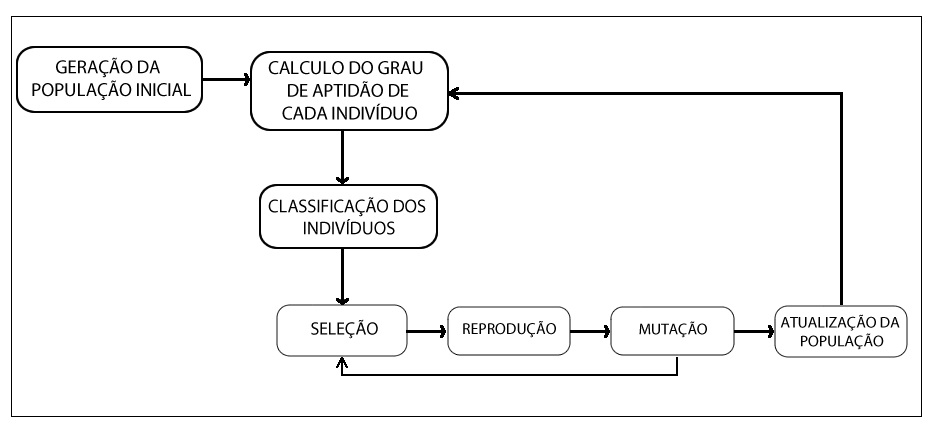
\includegraphics[scale=0.6]{./imagens/algoritimos_geneticos.jpg}}
	\caption[Demonstração da execução de um AG]
	{Demonstração da execução de um AG \textbf{Fonte:} Desenvolvido pelos autores.}
	\label{fig:representacao_ags}
\end{figure}

\par Como demostrado acima existem dois \texttt{loops}, o
\texttt{loop} que acontece até que uma nova população seja formada e outro
responsável por  iniciar a criação de uma nova população até que o
número de gerações seja atingido.

\subsubsection{População Inicial}

\par De acordo com \citeonline{livro_introduction_ag_melaine_mitchell}, a população inicial 
é o conjunto dos primeiros indivíduos candidatos à resolução do problema. Estes
indivíduos devem ser criados aleatoriamente, seguindo a lógica definida pelo programador com base no contexto do 
problema a ser resolvido. Um exemplo seria a população inicial do algoritmo desenvolvido neste trabalho, 
em que a população inicial será formada por possíveis formas de se produzir um determinado lote de calças, 
ou seja, será formada uma população de possíveis formas de dividir o trabalho entre as costureiras.

\subsubsection{Função de avaliação}

\par Segundo \citeonline{livro_ags_ricardo_linden}, após a criação da população
inicial, esta é então avaliada através de uma função de avaliação que mede a
qualidade de cada uma de suas soluções e é realizada então uma classificação que ordena as soluções das melhores para as
piores, para então iniciar a formação de uma nova população, a nova população
pode conter, já inicialmente, os dois melhores indivíduos existentes na
população inicial, este mecanismo é denominado elitismo e pode ser utilizado ou
não.

\par Ainda segundo o autor, a função de avaliação ou função de aptidão penaliza
as soluções inviáveis para a solução do problema, ou seja, ao verificar que uma
certa solução não satisfaz o grau de aptidão necessário para o problema
proposto, esta solução é descartada e, assim, só sobrevivem as soluções com mais
chance de resolver o problema e por isso torna-se o componente mais importante de qualquer algoritmo genético.

\par Devido à generalidade encontrada nos AGs, a função de avaliação
torna-se em muitos casos a única ligação verdadeira entre o programa e o
problema real pois ela irá analisar os cromossomos de cada indivíduo,
convertendo-os assim, em uma proposta de solução para o problema
\cite{livro_ags_ricardo_linden}.

% \par Baseando nessas \citeonline{livro_ags_ricardo_linden}, iremos
% usar no projeto uma função para avaliar dentre varias costureiras a melhor forma de
% destribuir a materia prima para que seja produzida uma certa quantidade de
% calças no menor tempo possível.


\subsubsection{Seleção}

\par Segundo \citeonline{livro_ags_ricardo_linden}, o próximo passo
para a formação da nova população é o cruzamento, que se inicia com a seleção de
dois indivíduos, que é realizada de acordo com a qualidade destes, porém,
como é fundamental que esta escolha não despreze completamente os indivíduos com uma
qualidade muito baixa, a seleção é feita de forma probabilística, ou seja,
indivíduos com boa qualidade possuem mais chances de serem selecionados e, por
outro lado, indivíduos com menor nota de avaliação terão menos chance se
reproduzirem.

\par O autor ressalta que a razão de o mecanismo de seleção não
escolher apenas as melhores soluções é devido ao fato de que aquelas com menor
grau de avaliação, também serem importantes para que se tenha uma maior diversidade de características
na população envolvida para a solução do problema, possibilitando assim
que esta possa evoluir de forma satisfatória, pois se as novas populações forem constituídas
somente das melhores soluções, elas serão compostas de indivíduos cada vez mais semelhantes
impedindo assim que novas soluções ainda melhores sejam concebidas.

\par Existem vários tipos de seleção. Um dos métodos utilizado para este fim é o método
roleta, muito utilizado entre a maioria dos pesquisadores de AGs. Metaforicamente, 
cada indivíduo da população ocupa uma porção da roleta, proporcional ao seu índice 
de aptidão, ou seja, os indivíduos que possuírem maior aptidão ocuparão uma maior 
porção do que aqueles com menor aptidão. A roleta, então, assim como mostra a
Figura ~\ref{fig:metodo_selecao_roleta}, é girada e o indivíduo escolhido é
aquele em que a seta parar sobre ele \cite{REVISTA_MULTIDISCIPLINAR_DA_UNIESP}.


\begin{figure}[h!]
	\centerline{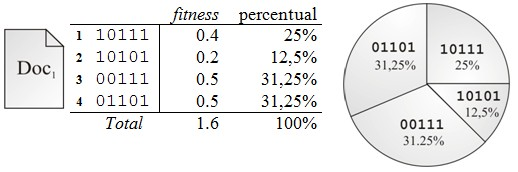
\includegraphics[scale=1.0]{./imagens/roleta.jpg}}
	\caption[Demonstração do método de seleção Roleta]
	{Demonstração do método de seleção Roleta \textbf{Fonte:}
	"http://www.dgz.org.br/fev09/Art04.htm".}
	\label{fig:metodo_selecao_roleta}
\end{figure}



\subsubsection{Cruzamento} 

\par Segundo \citeonline{livro_ags_ricardo_linden}, após a seleção dos pais, irá
ocorrer então o processo de cruzamento ou \textit{crossover} e, como no cruzamento natural, neste processo dois novos indivíduos, ou seja, duas
novas soluções são formadas a partir de características daquelas que se
cruzaram, ou seja, serão geradas duas novas soluções que conterão alguns cromossomos
de uma solução e alguns cromossomos de outra.

\par Para \citeonline{intro_aos_algoritimos_geneticos}, o operador
\textit{crossover} é um mecanismo de busca dos AGs para explorar regiões
desconhecidas do espaço de busca. Ele é aplicado a cada par de cromossomos dos
indivíduos que passaram pelo processo de seleção, gerando assim, dois novos
indivíduos.

\par Para \citeonline{REVISTA_MULTIDISCIPLINAR_DA_UNIESP}, o cruzamento combina
os cromossomos pais a fim de gerar cromossomos filhos e para isso existem vários
tipos de cruzamento.

\par Um dos cruzamentos muito utilizado é o cruzamento de um ponto, que divide a
lista de cromossomos selecionados em um ponto de sua cadeia, esse ponto é escolhido aleatoriamente.
Após essa divisão, é copiada uma parte dos cromossomos de cada pai para definir
os cromossomos dos indivíduos filhos. Neste método, é comum os pais gerarem dois
novos filhos \cite{REVISTA_MULTIDISCIPLINAR_DA_UNIESP}.

\par Um outro cruzamento muito utilizado é o cruzamento uniforme, que
ainda segundo o autor, gera cada gene do descendente copiando o gene em questão
de um dos pais, em que se usa uma máscara de cruzamento que é gerada aleatoriamente para fazer a escolha.
Para criar cada cromossomo do novo indivíduo é feita uma iteração em todas as
posições da máscara fazendo uma análise dos seus valores, quando o valor da posição for 1, o gene do
primeiro pai referente à mesma posição da máscara é copiado, se o valor for 0
será copiado o gene do segundo pai, depois desse processo é gerado o novo
descendente.

\par Segundo \citeonline{intro_aos_algoritimos_geneticos}, o tipo de cruzamento
uniforme difere do cruzamento de um ponto uma vez que este sempre leva à
metade dos \textit{bits} de cada pai.

\subsubsection{Mutação}

\par Para \citeonline{livro_ags_ricardo_linden}, também pode ocorrer a mutação em
que, como ocorre na natureza, aleatoriamente o valor dos
cromossomos de um indivíduo pode ser alterado. A mutação ocorre de acordo com
uma taxa definida. Basicamente é definida uma porcentagem baixa e então um
número de 0 a 1 é sorteado e multiplicado por 100, se o resultado for menor que
a porcentagem definida, irá ocorrer a mutação para aquele indivíduo.

\par Para \citeonline{intro_aos_algoritimos_geneticos}, a mutação melhora a
diversidade dos cromossomos na população. Em contrapartida, depois de realizada
a mutação se perdem as informações contidas no cromossomo. Assim, para assegurar
a diversidade deve-se usar uma taxa de mutação pequena. 


\par Assim como no cruzamento há vários tipos de mutação, dentre eles a mutação
de \textit{bit} que é um tipo de mutação mais simples de ser implementada.

\par Segundo \citeonline{REVISTA_MULTIDISCIPLINAR_DA_UNIESP} este é o operador
mais fácil de trabalhar podendo ser aplicado em qualquer forma de representação
binária dos cromossomos. Este tipo de mutação gera uma probabilidade de mutação
para cada \textit{bit} do cromossomo, caso a probabilidade sorteada estiver
dentro da taxa de mutação definida, o \textit{bit} sofrerá mutação, recebendo um
valor determinado de forma aleatória dentre os valores que podem ser assumidos pelo cromossomo.


\par No problema a ser solucionado na aplicação deste trabalho, há um
cenário em que existem diversas soluções para se resolver o problema e deseja-se
encontrar a melhor dentre elas. Conforme descrito anteriormente, os AGs são uma
das melhores opções para se resolver este tipo de problema, por este motivo esta técnica foi escolhida.

% \par Para \citeonline[p.4]{ifsudestemg}, a proposta da Orientação a
% Objetos é,
% 
% \begin{citacao}
% Representar o mais fielmente possível as
% situações do mundo real nos sistemas computacionais. Nós entendemos o mundo
% como um todo composto por vários objetos que interagem uns com os outros. Da
% mesma maneira, a Orientação a Objetos consiste em considerar os sistemas
% computacionais não como uma coleção estruturada de processos, mas sim como
% uma coleção de objetos que interagem entre si.
% \end{citacao}  


% 
% Este processo é iniciado com um conjunto de várias soluções
% candidatas que fazem alusão aos cromossomos e cada solução possui atributos que
% definem como o problema pode ser resolvido. Tais atributos fazem alusão aos
% genes e os valores que estes atributos podem assumir, seja um valor numérico,
% ou um texto, por exemplo, fazem referência aos alelos. Após estas definições 
% durante a execução do algoritmo, ocorre o processo de reprodução em que as
% soluções se cruzam entre si, simulando o processo de \textit{crossing-over} no
% intuito de gerarem soluções possivelmente melhores, alem disto também é simulado
% o processo de mutação em que aleatóriamente um atributo de uma solução pode ser alterado.
% No final deste processo existe um mecanismo que mede a qualidade das soluções
% geradas e o processo continua até que a melhor solução seja encontrada ou até que o número
% de reproduções, definido préviamente, seja atingido, neste caso a melhor solução
% encontrada até aquele momento será o resultado do processo, ou seja, a melhor
% solução naquela execução, sendo importante ressaltar porém que outras execuções
% podem gerar resultados diferentes. \cite{livro_introduction_ag_melaine_mitchell}


\section{Tecnologias}

\par Abaixo serão listadas as tecnologias que serão utilizadas no
desenvolvimento do projeto.

\subsection{Linguagem de programação Java}

\par Segundo \citeonline{oracle}, a Linguagem Java foi projetada
para permitir o desenvolvimento de aplicações seguras, portáteis
e de alto desempenho para a mais ampla gama de plataformas de computação.

\par De acordo com \citeonline{livro_java_complete_references}, o Java foi
criado em 1991 pela \textit{Sun Microsystems} e foi baseado em uma linguagem já
existente, o C++, que foi escolhida por ser orientada a objetos e
por gerar códigos compactados, o que era exatamente o que eles precisavam para
implantar em pequenos aparelhos. Além dessas características, um requisito
desejável era que a nova linguagem fosse independente de plataforma, para que
fosse executado em qualquer arquitetura, tais como, TVs, telefones, entre
outros, e então, para atender esta exigência, foi
criado o conceito de máquina virtual, que ficou conhecido como \textit{Java
Virtual Machine} - JVM\footnotemark[2].

\footnotetext[2]{O termo Java Virtual Machine será referenciado pela sigla JVM a
partir deste ponto do trabalho.}

\par O ponto chave que
permite o Java resolver o problema de portabilidade é o fato de o código ser
compilado em \textit{Bytecode}, que é um conjunto genérico de instruções
altamente otimizado que é executado pela JVM, e esta, por sua vez, traduz o
mesmo para a arquitetura a qual ela está instalada o que possibilita a execução do programa
em várias plataformas \cite{livro_java_complete_references}.
%Ver este contexto resolvendo assim também problemas associados com programas baseados na web. 


% 
% \par Hoje os Browsers que possuem JVM embutida podem executar programas que 
% utilizam a linguagem JAVA. 
% 
% Neste particular Quinteiro (2006) registrou que:
% 
% \begin{citacao}
% “A Sun considera o sucesso do Java na Internet como sendo o primeiro passo para utilizá-lo em decodificadores da 
% televisão interativa, em dispositivos portáteis e outros produtos eletrônicos de consumo - exatamente como o Java 
% tinha começado em 1991. Sua natureza portátil e o projeto robusto permitem o desenvolvimento para múltiplas 
% plataformas, em ambientes tão exigentes como os da eletrônica de consumo".\cite[p.33]{livro_ags_ricardo_linden}
% \end{citacao}  


\par Além da portabilidade, o Java também é \textit{multithread}, ou seja,
permite a execução de múltiplas tarefas simultaneamente. A linguagem também
conta com um \textit{automatic garbage collector} que consiste em um mecanismo
de gerenciamento e limpeza de memória que a JVM acomoda. Além disso o Java
suporta uma extensa biblioteca de rotinas que facilitam a interação com protocolos 
TCP/IP, como HTTP e FTP \cite{livro_java_complete_references}.

\par De acordo com \citeonline{livro_java_Guia_do_Programador}, 

\begin{citacao} Atualmente a linguagem está organizada em três segmentos
principais:


	- JavaMe (\textit{Java Micro Edition}) - Destinado a pequenos dispositivos
	computacionais móveis, tais como celulares, PDAs e \textit{set-top boxes}. É
	composto de máquina virtual otimizada para ambientes mais restritos, com
	especificações de funcionalidades e uma API mais compacta;
	  
	- JavaSE (\textit{Java Standard Edition}) - Integra os elementos padrão
	da plataforma e permite o desenvolvimento de aplicações de pequeno e médio porte. Inclui todas as APIs consideradas de base,
além da máquina virtual padrão;

	- JavaEE (\textit{Java Enterprise Edition}) - Voltada para o desenvolvimento
	de aplicações corporativas complexas. Adiciona APIs específicas aos elementos
	padrão da plataforma.
	

\end{citacao}


\par Para \citeonline{livro_intro_a_prog_orientada_objetos_usando_java}, Java é
uma linguagem Orientada a Objetos (OO), este paradigma usa objetos, criados a
partir de modelos, também chamados de classes, para representar e processar
dados em aplicações computacionais. Basicamente uma classe ou modelo é um
conjunto de especificações de um objeto, ou seja, que tipo de dados este deve
ter e quais operações este terá e então após a criação da classe o programador
pode criar um objeto desta. Uma analogia simples seria a planta de uma casa e a
construção da mesma em si, a planta representa a classe, ou seja, como a casa deve ser feita e a casa depois de construída representa o objeto.

\par Os dados e operações são guardados em objetos e estes são os elementos
centrais do programa. Assim a aplicação como um todo é vista como uma coletânea
de objetos que se relacionam uns com os outros. Cada objeto representa um conceito real de uma parte do problema. 
Isto permite que o desenvolvimento se torne menos complexo pois os conceitos são familiares
às pessoas envolvidas no projeto pelo fato de que a aplicação não está
organizada em processos estruturados mas sim em objetos que espelham o mundo real e interagem entre si  \cite{teste_doutorado_manzoni}.

\par Para \citeonline{livro_intro_a_prog_orientada_objetos_usando_java}, 
os dados pertencentes aos modelos são representados por tipos nativos,
característicos das linguagem de programação e podem também ser representados
por outros modelos criados pelo programador.

%\par O autor ainda exemplifica um modelo como a representação de um funcionário
% de uma empresa para fins de processamento de folha de pagamento. Neste caso o
%modelo representaria dentre outros dados, o nome, cargo, salário e horas extras
% trabalhadas dessa pessoa, e as operações seria aquelas relacionados com realização
% de cálculos de salário e impostos, por exemplo.

\par Para o desenvolvimento do sistema de informação deste projeto, o paradigma
de orientação a objetos, que será implementado na linguagem Java, será
imprescindível devido à alta complexidade do problema a ser resolvido. Pois cada objeto representará partes do algoritmo genético que será desenvolvido, tais
como a representação do Indivíduo, Cromossomos, etc, o que facilitará muito o
desenvolvimento.

\par O produto resultante deste trabalho faz uso do Java EE e, como já foi dito
em seções anteriores, será implementado em plataforma WEB. Para tal, faz-se
necessário o uso de um servidor de aplicações WEB. Dentre as opções disponíveis, foi escolhido o \textit{Tomcat} pelo fato de este ser o mais simples e ter os atributos mínimos necessários para a aplicação que
será desenvolvida.

\par Segundo \citeonline{livro_apache_tomcat_7}, o \textit{Tomcat} é um
servidor \textit{open source} e \textit{container} de aplicações \textit{web}
baseados em Java. Ele foi criado para executar \textit{servlets}, que também é
uma denominação para classe dentro da especificação do Java para WEB, e arquivos
de marcação que definem os elementos visuais da tela que será explanado na seção.
O \textit{Tomcat} foi criado como um subprojeto da \textit{Apache-Jakarta}, porém como ficou
muito popular entre os desenvolvedores, a \textit{Apache} o denominou como um
projeto separado e vem sendo melhorado e apoiado por um grupo de voluntários da comunidade \textit{Java Open Source}, que o faz 
uma excelente solução para desenvolvimento de uma aplicação \textit{web} completa. 

 

\subsection{Interface Gráfica - JSF}


\par Para a construção da interface gráfica (páginas web) da aplicação
desenvolvida neste trabalho, foi utilizado um \textit{framework} nativo nas
novas versões do Java denominado \textit{Java Server Faces} (JSF).

\par \citeonline{bergsten_javaserver_faces} afirma que o JSF é um
\textit{framework server-side} baseado em componentes \textit{web}, cuja principal função é abstrair os detalhes de manipulação dos eventos e organização dos componentes na página \textit{web}. 
Por meio dele, é possível desenvolver páginas mais sofisticadas de forma
simples, abstraindo, inclusive, o tratamento de requisições e respostas. Isto permite ao desenvolvedor focar-se no \textit{back-end} da aplicação, ou seja, na lógica, e não se preocupar com detalhes a respeito de requisições e respostas HTTP e como obter as informações recebidas e/ou enviadas através deste protocolo.

\par De acordo com \citeonline{oracle_javaserver_faces_technology_overview}, o
JSF é de fácil aprendizado e utilização, pois possui sua arquitetura claramente definida, sendo dividida entre a lógica da aplicação e apresentação. Esta divisão é possível pois ele utiliza o padrão de projeto \textit{Model-View-Controller} - MVC\footnotemark[3], tornando-o um importante \textit{framework} para desenvolvimento de aplicações utilizando a plataforma Java \textit{Web}.

\footnotetext[3]{MVC: \textit{Model-View-Controller} - \textit{Design
pattern}, padrão de arquitetura de software que separa a informação (e as suas
regras de negócio) da interface com a qual o usuário interage.}

%BANCA_QUALIFICACAO. Comentado este parágrafo, porém o mesmo retornará para a banca de qualificação
\par Segundo
\citeonline{gamma_helm_johnson_vlissides_design_patterns_elements_reusable_object_oriented_software}, 
o padrão de projeto MVC é dividido em três partes. O \textit{Model} é a lógica e
acesso aos dados da aplicação, a \textit{View} é camada de apresentação e por
último o \textit{Controller} é responsável por definir a interface entre a lógica e a apresentação. Portanto, todo tipo de requisição ou resposta deve ser obrigatoriamente enviada 
ao \textit{Controller}, que, por sua vez encaminhará para a camada de visão ou
de lógica. A Figura ~\ref{fig:modelo_mvc} demonstra um exemplo do modelo MVC
utilizando o JSF.

% Imagem do modelo MVC usando JSF - VOLTAR PARA A BANCA DE QUALIFICACAO
\begin{figure}[h!]
	\centerline{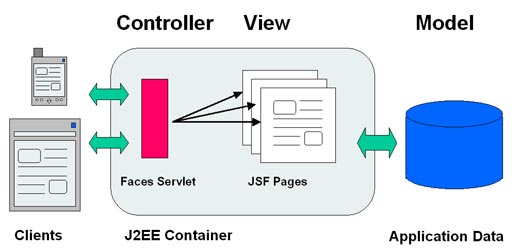
\includegraphics[scale=0.5]{./imagens/jsf_using_mvc.jpg}}
	\caption[Demonstração do Modelo MVC]
	{Demonstração do Modelo MVC. \textbf{Fonte:}
	http://www.javabeat.net/jsf-2/.}
	\label{fig:modelo_mvc}
\end{figure}

%BANCA_QUALIFICACAO. Comentado este parágrafo, porém o mesmo retornará para a banca de qualificação
\par Ao utilizar o JSF, toda e qualquer interação que o usuário realizar com a aplicação será executada por 
um \textit{servlet} chamado \textit{Faces Servlet}. Ele é a responsável por
receber tais requisições da camada de visão e redirecioná-las à lógica da aplicação e, posteriormente, enviar a resposta ao 
usuário \cite{faria_java_ee_7_jsf_primefaces_cdi}.

\par Segundo \citeonline{livro_programacao_java_para_web}, a especificação do \textit{JavaServer
	Faces} foi definida pela \textit{Java Comunity Process} - JCP\footnotemark[4],
	que é uma entidade cujo objetivo é especificar a evolução do Java. E por este motivo grandes empresas como
\textit{Apache}, \textit{IBM}, \textit{Oracle}, entre outras, participaram
desta definição. As implementações mais conhecidas são da especificação do JSF são:

\footnotetext[4]{O termo \textit{Java Comunity Process} será referenciado pela
	sigla JCP a partir deste ponto do trabalho.}

\begin{itemize}
	\item \textit{Sun Mojarra} (antes JSF R1) – implementação de referência
	(\url{http://javaserverfaces.java.net/})
	
	\item \textit{MyFaces} da \textit{Apache} (\url{http://myfaces.apache.org/})
\end{itemize}

\par Com essas implementações é possível utilizar todos os recursos do padrão JSF,
como formulários, tabelas, \textit{layout}, conversão e validação de eventos,
além de toda a inteligência para a interpretação dos arquivos de configuração e
interação com o \textit{container} Java. Como o JSF é um padrão de mercado,
várias empresas investem no desenvolvimento de bibliotecas de componentes como, calendário, barras de progresso, menus,
efeitos de transição entre outros \cite{livro_programacao_java_para_web}.

\par Algumas das principais bibliotecas de componentes são:

\begin{itemize}
	\item \textit{Trinidad}, da \textit{Apache MyFaces}
	(\url{http://myfaces.apache.org/trinidad/});
	
	\item \textit{Tobago}, da \textit{Apache MyFaces}
	(\url{http://myfaces.apache.org/tobago/});
	
	\item \textit{ICEFaces}, da \textit{ICESoft} (\url{http://www.icefaces.org/});
	
	\item \textit{RichFaces}, da \textit{JBoss}
	(\url{http://www.jboss.org/richfaces/});
	
	\item \textit{Tomahawk}, da \textit{Apache MyFaces}
	(\url{http://myfaces.apache.org/tomahawk/});
	
	\item \textit{PrimeFaces} (\url{http://www.primefaces.org/}).
\end{itemize}

\par Neste trabalho, é utilizada a biblioteca PrimeFaces, que é uma
biblioteca de componentes que implementa a especificação do JSF. Ele possui uma ampla gama de componentes disponíveis 
para auxiliar o desenvolvimento de interfaces \textit{web} ricas, além de possuir o seu
código fonte aberto \cite{ross_borsoi_uso_primefaces}.

\par Para \citeonline{juneau_primefaces_enterprise}, uma das grandes vantagens
do Primefaces é a facilidade de integração entre ele e o JSF, bastando apenas
incluir a biblioteca do Primefaces no projeto JSF, salvo alguns componentes
específicos, como o \textit{file upload}, que necessita de pequenas configurações adicionais.
Essas mudanças, quando necessárias, devem ser realizadas no arquivo de
configuração da aplicação que, por padrão, é chamado de \textit{web.xml}, porém,
o mesmo pode ser alterado pelo desenvolvedor.

\par Por possuir as vantagens descritas acima e uma simples configuração, além de ser um 
\textit{framework cross-browser\footnotemark[5]}, o JSF foi escolhido para
auxiliar no desenvolvimento das páginas \textit{web} deste trabalho.

% E por todas as vantagens do Primefaces mencionadas, somado ao fato de esta
% biblioteca possuir uma ótima documentação em conjunto com uma grande comunidade de desenvolvedores que a 
% utilizam e a alta demanda de desenvolvedores que a conhecem no mercado, ela foi
% escolhida em conjunto com o JSF para desenvolvimento das páginas \textit{web}
% deste trabalho.

\footnotetext[5]{\textit{Cross-Browser} - Compatibilidade com todos os tipos de
dispositivos e navegadores}

% \par O \textit{Apache Tomcat} é um servidor web estável, ele 
% possui varias funcionalidades como o \textit{Tomcat Manager},
% \textit{Specialized Realm Implementations} e \textit{Tomcat Valves}. O
% \textit{Tomcat Manager} é fornecido com o servidor \textit{Tomcat} e é
% responsável pela funcionalidade básica para gerenciar aplicações web em execução no servidor \textit{Tomcat} 
% a partir de qualquer navegador. Ja o \textit{Specialized Realm Implementations}
% é um método de segurança que o Tomcat disponibiliza para proteger os recursos
% dentro do \textit{container} que é um recipiente que funciona como um banco de
% dados de usuários e esses bancos são denominados \textit{Realm}. O
% \textit{Tomcat Valves} é uma tecnologia que foi introduzido no Tomcat 4 e esta disponível nas versões
% posteriores e permitem associar instâncias de uma classe JAVA com um
% \textit{container} \textit{Catalina} particular, agindo como um pré-processador
% para todos os pedidos que vêm para o \textit{container}. 
% \cite{livro_apache_tomcat_7}



%\par Segundo a Apache (2015), o Tomcat é um software livre que realiza a
%implementação de especificações do Java voltado para programação para 
%internet lançado pela própria Apache.
% \par Exemplo de parágrafo utilizando comando para formatar em itálico as palavras em inglês, como por exemplo: \textit{pets, animals and software} e um exemplo de texto em negrigo: \textbf{grafo}.
% 
% \par Um tipo de citação: segundo \citeonline{correa2003plantas} as plantas \ldots.
% 
% \par Outro tipo de citação: as plantas \ldots \cite{correa2003plantas}.
% 
% \par Outro tipo de citação com página: \cite[p. 13]{correa2003plantas}.
% \par Outro tipo ainda de citação com página:  \citeonline[p. 13]{correa2003plantas}.
% 
% \par Para referenciar seções e capítulos, é necessário colocar o \textbackslash label e a referência assim: na \autoref{sec:materiais} e no \autoref{cap:quadroMetodologico} são encontradas as informações\ldots
% 
% \par Exemplo de equação:
% 
% \begin{equation}
%  \Delta Q = 
%  \left[
%  \frac{\sum_{in} + k_{i,in}}{2m} - 
%  \left(
%  \frac{\sum_{tot} + k_i}{2m}
%  \right)^2
%  \right] -
%  \left[
%  \frac{\sum_{in}}{2m} - 
%  \left(\frac{\sum_{tot}}{2m}
%  \right)^2 - 
%  \left(\frac{k_i}{2m}
%  \right)^2
%  \right]
% \end{equation}
% 
% 
% \par Símbolos matemáticos só funcionam dentro do ambiente \texttt{equation} ou entre dois símbolos \$. Ex: Adiciona cada vértice $w \in N_d(v) \Delta \Gamma$ na região, os quais foram vistos por pelo menos a uma fração $\gamma$ dos vértices em $N_d(v)$.
% 
% \par Outra fórmula: $y=x^2$
% 
% \section{Materiais}
% \label{sec:materiais}
% 
% \par Este parágrafo mostra um exemplo de um teste de nota de rodapé, utilizando o texto do documento da Univas\footnote{O nome “Desenvolvimento” é muito vago, portanto, não o utilize; prefira, de acordo com a situação, ``Fundamentação teórica'', ``Análise dos dados'', ``Objetivos'', ``Metodologia'', etc. }. Outro tipo de nota de rodapé\footnote{\cite{correa2003plantas}}.  Outro tipo ainda de nota de rodapé\footnote{\citeonline{correa2003plantas}}
% 
% 
% \par Um exemplo de tabela é mostrado na Tabela~\ref{tab:informativa}
% 
% 
% \begin{table} [h]
%   \caption[Informação nutricioal dos alimentos]
%           {Informação nutricioal dos alimentos \textbf{Fonte:} \cite{correa2003plantas}}
%   \centering
%   \begin{tabular}{|p{0.7in}|p{2in}|p{3in}|}
%     \hline 
%     \multicolumn{1}{|c|}{\textbf{Hortaliça}} & \multicolumn{1}{c|}{\textbf{Valor Nutricional}} & \multicolumn{1}{c|}{\textbf{Propriedades medicinais}} \\
%     \hline 
% Tomate
% &Vitamina A, C, E e ferro, potássio
% &Maior resistência aos vasos sanguíneos, combate a infecções\\
%     \hline 
% Cenoura
% &Vitamina A, vitaminas do complexo B, cálcio, fósforo
% &Regula o aparelho digestivo, purifica a bile e fortalece a pele\\
%     \hline
% Cebolinha
% &Cálcio, ferro, niacina
% &Estimula o apetite, ajuda na formação de ossos e dentes\\
% 
%     \hline
% Alface
% &Ferro, cálcio, niacina, vita\-mina C
% &Combate insônia, ajuda na cicatrização dos tecidos\\
% 
%     \hline
% Rúcula
% &Iodo, vitaminas A e C
% &Combate a fadiga, depura o sangue\\
% 
%     \hline
% Erva cidreira
% &Sais minerais
% &Tonico nervoso, combate cólicas intestinais\\
% 
%     \hline 
%   \end{tabular}
%   \legend{Fonte: \cite{correa2003plantas}}
%   \label{tab:informativa}
% \end{table}
% 
% \par A seguir segue exemplo de listagem numérica:
% 
% \begin{enumerate}
%   \item conteúdo do item 1;
%   \item conteúdo do item 2;
%   \item conteúdo do item 3;
%   \item conteúdo do item 4;
%   \item conteúdo do item 5;
%   \item conteúdo do item 6;
%   \item etc.
% \end{enumerate}
% 
% \par Também é possível fazer a lista de itens:
% 
% \begin{itemize}
%   \item conteúdo do primeiro item;
%   \item conteúdo do segundo item;
%   \item conteúdo do terceiro item;
%   \item conteúdo do quarto item;
%   \item conteúdo do quinto item;
%   \item etc.
% \end{itemize}
% 
% \par Um exemplo de imagem é mostrado na Figura~\ref{fig:exemplo1}.
% 
% \begin{figure}[h!]
%   \centerline{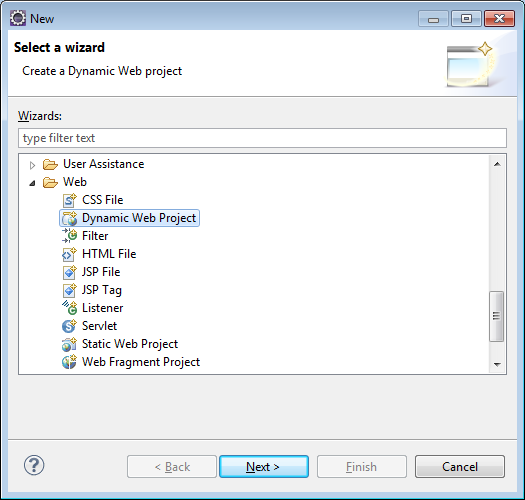
\includegraphics[scale=0.65]{./imagens/apendice_img1.png}}
%   \caption[Exemplo de criação de um projeto Web no Eclipse]
%           {Exemplo de criação de um projeto Web no Eclipse. \textbf{Fonte:} \cite{correa2003plantas}}
% \label{fig:exemplo1}
% \end{figure}
% 
% \par Perceba que o \LaTeX~faz a numeração automática das figuras e já adiciona na lista de figuras.
% 
% \par Agora a mesma imagem foi incluída, porém em escala menhor, conforme ilustra a Figura~\ref{fig:exemplo2}.:
% 
% \begin{figure}[h!]
%   \centerline{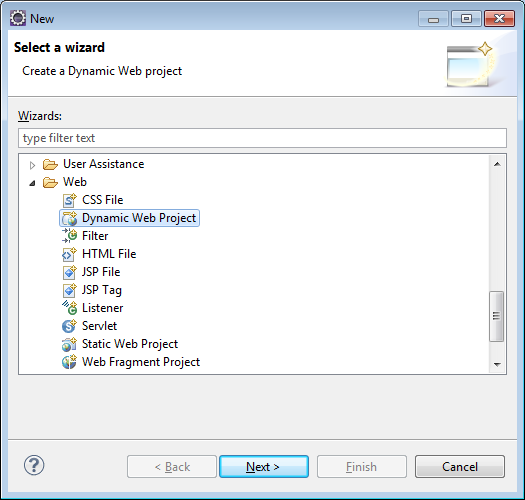
\includegraphics[scale=0.25]{./imagens/apendice_img1.png}}
%   \caption[Mesma imagem em escala menor]
%           {Mesma imagem em escala menor. \textbf{Fonte:} \cite{correa2003plantas}}
% \label{fig:exemplo2}
%\end{figure}


\subsection{Armazenamento de dados}

\par A aplicação desenvolvida neste trabalho irá demandar o armazenamento de
informações das costureiras e da disponibilidade das mesmas. Além disso, as saídas
oferecidas pelo algoritmo genético deverão ser armazenadas para uso posterior,
alimentando, assim, a base de dados do sistema, fazendo-se necessário o
uso de um banco de dados.

\par O gerenciador de banco de dados a ser utilizado nesta aplicação é o PostgreSQL, que 
foi escolhido por ser uma ferramenta robusta e \textit{open source}. O
PostgreSQL é um banco de dados relacional desenvolvido pela universidade da California por volta de 1970. Na
época, o projeto se chamava Ingres e só passou a se chamar Postgres por volta de 1986 quando Michael Stonebraker adicionou
o conceito de orientação a objetos ao projeto e decidiu então definir um novo
nome para a nova versão \cite{livro_postgres_doulgas}.

\par Para \citeonline{livro_introd_sistemas_bd} , ``um banco de dados é um
sistema computadorizado cuja funcionalidade geral é armazenar informações e
permitir que os usuários busquem e atualizem essas informações quando as
solicitar''. Já o conceito de banco de dados relacional é definido por
\citeonline[p.30]{oracle_database_sql} como:
\begin{citacao}
uma coleção de informações relacionadas, organizadas em tabelas. Cada tabela
armazena dados em linhas; os dados são organizados em colunas. As tabelas são
armazenadas em esquemas de banco de dados, que são áreas  onde os usuários 
podem armazenar suas próprias tabelas.
\end{citacao}
 \par Para manipular e acessar as informações em um banco de dados relacional
 é usada uma linguagem denominada SQL (\textit{Structured Query Language}), que
 foi projetada  especificamente para este fim. A linguagem foi desenvolvida
 pela IBM por volta de 1970 que tomou como base o trabalho do Dr. Edgar Frank
 Codd e possui uma sintaxe simples de fácil aprendizado e utilização \cite{oracle_database_sql}.


%\par Segundo a Apache (2015), o Tomcat é um software livre que realiza a
%implementação de especificações do Java voltado para programação para 
%internet lançado pela própria Apache.
% \par Exemplo de parágrafo utilizando comando para formatar em itálico as palavras em inglês, como por exemplo: \textit{pets, animals and software} e um exemplo de texto em negrigo: \textbf{grafo}.
% 
% \par Um tipo de citação: segundo \citeonline{correa2003plantas} as plantas \ldots.
% 
% \par Outro tipo de citação: as plantas \ldots \cite{correa2003plantas}.
% 
% \par Outro tipo de citação com página: \cite[p. 13]{correa2003plantas}.
% \par Outro tipo ainda de citação com página:  \citeonline[p. 13]{correa2003plantas}.
% 
% \par Para referenciar seções e capítulos, é necessário colocar o \textbackslash label e a referência assim: na \autoref{sec:materiais} e no \autoref{cap:quadroMetodologico} são encontradas as informações\ldots
% 
% \par Exemplo de equação:
% 
% \begin{equation}
%  \Delta Q = 
%  \left[
%  \frac{\sum_{in} + k_{i,in}}{2m} - 
%  \left(
%  \frac{\sum_{tot} + k_i}{2m}
%  \right)^2
%  \right] -
%  \left[
%  \frac{\sum_{in}}{2m} - 
%  \left(\frac{\sum_{tot}}{2m}
%  \right)^2 - 
%  \left(\frac{k_i}{2m}
%  \right)^2
%  \right]
% \end{equation}
% 
% 
% \par Símbolos matemáticos só funcionam dentro do ambiente \texttt{equation} ou entre dois símbolos \$. Ex: Adiciona cada vértice $w \in N_d(v) \Delta \Gamma$ na região, os quais foram vistos por pelo menos a uma fração $\gamma$ dos vértices em $N_d(v)$.
% 
% \par Outra fórmula: $y=x^2$
% 
% \section{Materiais}
% \label{sec:materiais}
% 
% \par Este parágrafo mostra um exemplo de um teste de nota de rodapé, utilizando o texto do documento da Univas\footnote{O nome “Desenvolvimento” é muito vago, portanto, não o utilize; prefira, de acordo com a situação, ``Fundamentação teórica'', ``Análise dos dados'', ``Objetivos'', ``Metodologia'', etc. }. Outro tipo de nota de rodapé\footnote{\cite{correa2003plantas}}.  Outro tipo ainda de nota de rodapé\footnote{\citeonline{correa2003plantas}}
% 
% 
% \par Um exemplo de tabela é mostrado na Tabela~\ref{tab:informativa}
% 
% 
% \begin{table} [h]
%   \caption[Informação nutricioal dos alimentos]
%           {Informação nutricioal dos alimentos \textbf{Fonte:} \cite{correa2003plantas}}
%   \centering
%   \begin{tabular}{|p{0.7in}|p{2in}|p{3in}|}
%     \hline 
%     \multicolumn{1}{|c|}{\textbf{Hortaliça}} & \multicolumn{1}{c|}{\textbf{Valor Nutricional}} & \multicolumn{1}{c|}{\textbf{Propriedades medicinais}} \\
%     \hline 
% Tomate
% &Vitamina A, C, E e ferro, potássio
% &Maior resistência aos vasos sanguíneos, combate a infecções\\
%     \hline 
% Cenoura
% &Vitamina A, vitaminas do complexo B, cálcio, fósforo
% &Regula o aparelho digestivo, purifica a bile e fortalece a pele\\
%     \hline
% Cebolinha
% &Cálcio, ferro, niacina
% &Estimula o apetite, ajuda na formação de ossos e dentes\\
% 
%     \hline
% Alface
% &Ferro, cálcio, niacina, vita\-mina C
% &Combate insônia, ajuda na cicatrização dos tecidos\\
% 
%     \hline
% Rúcula
% &Iodo, vitaminas A e C
% &Combate a fadiga, depura o sangue\\
% 
%     \hline
% Erva cidreira
% &Sais minerais
% &Tonico nervoso, combate cólicas intestinais\\
% 
%     \hline 
%   \end{tabular}
%   \legend{Fonte: \cite{correa2003plantas}}
%   \label{tab:informativa}
% \end{table}
% 
% \par A seguir segue exemplo de listagem numérica:
% 
% \begin{enumerate}
%   \item conteúdo do item 1;
%   \item conteúdo do item 2;
%   \item conteúdo do item 3;
%   \item conteúdo do item 4;
%   \item conteúdo do item 5;
%   \item conteúdo do item 6;
%   \item etc.
% \end{enumerate}
% 
% \par Também é possível fazer a lista de itens:
% 
% \begin{itemize}
%   \item conteúdo do primeiro item;
%   \item conteúdo do segundo item;
%   \item conteúdo do terceiro item;
%   \item conteúdo do quarto item;
%   \item conteúdo do quinto item;
%   \item etc.
% \end{itemize}
% 
% \par Um exemplo de imagem é mostrado na Figura~\ref{fig:exemplo1}.
% 
% \begin{figure}[h!]
%   \centerline{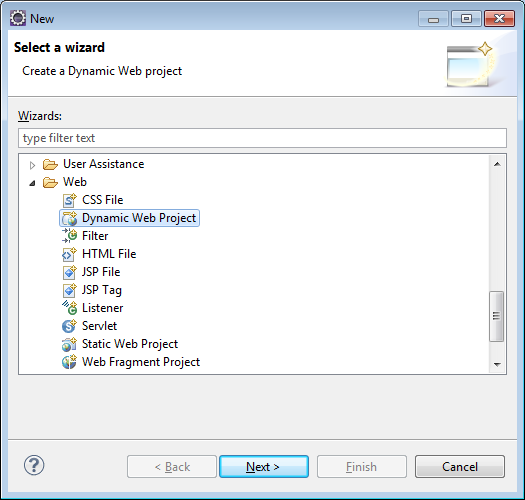
\includegraphics[scale=0.65]{./imagens/apendice_img1.png}}
%   \caption[Exemplo de criação de um projeto Web no Eclipse]
%           {Exemplo de criação de um projeto Web no Eclipse. \textbf{Fonte:} \cite{correa2003plantas}}
% \label{fig:exemplo1}
% \end{figure}
% 
% \par Perceba que o \LaTeX~faz a numeração automática das figuras e já adiciona na lista de figuras.
% 
% \par Agora a mesma imagem foi incluída, porém em escala menhor, conforme ilustra a Figura~\ref{fig:exemplo2}.:
% 
% \begin{figure}[h!]
%   \centerline{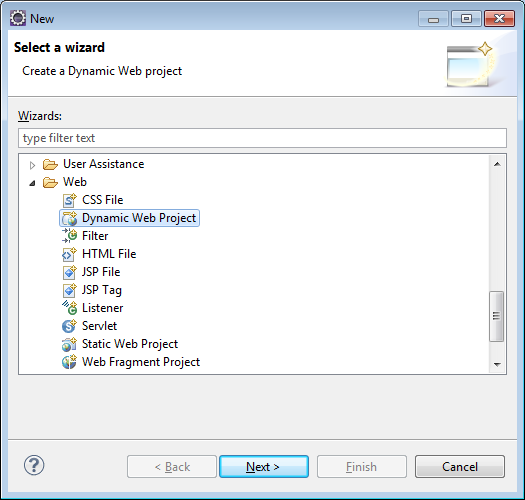
\includegraphics[scale=0.25]{./imagens/apendice_img1.png}}
%   \caption[Mesma imagem em escala menor]
%           {Mesma imagem em escala menor. \textbf{Fonte:} \cite{correa2003plantas}}
% \label{fig:exemplo2}
%\end{figure}



% \par    Desta forma surge a necessidade de primeiramente descrever os
% princípios da teoria proposta por Darwin para que se possa ter um melhor
% entendimento do contexto de computação evolucionária e de algoritmos genéticos.
% É importante, porém, ressaltar que o conteúdo desta sessão não tem como
% objetivo levantar questões sobre o tema da origem dos seres vivos. 
% 	
% \par	O autor afirma ainda que o trabalho de Darwin iniciou-se p
% Esta observação foi o ponto chave que levou o inglês a criar a teoria da evolução. 
% 	
% \par 	Ainda segundo Linden, a teoria afirma que,  

% \par algoritmos genéticos são um ramo de uma das abordagens da inteligência
% artificial denominada abordagem evolutiva. Segundo Lacerda e Carvalho o termo,
% proposto inicialmente por John Holland em 1975 e popularizado através de seu aluno Goldberg
% em 1989, está fundamentado no princípio de seleção natural proposto por Charles Darwin em seu
% livro A Origem das Espécie.
% 
% \par Darwin (1859) propôs que os indivíduos mais fortes evoluem através do processo de
% seleção natural, que define que o indivíduos com melhor capacidade de adaptação ao seu
% ambiente possuem maior chance de sobreviver e gerar descendentes. Algoritmos genéticos
% seguem este mesmo conceito, pois, segundo \citeonline{livro_ags_ricardo_linden},
% são um ramo de um modelo computacional conhecido como algoritmos evolucionários e como tal definem­se como uma
% técnica de otimização e busca que se baseia na teoria do processo de evolução
% natural. \citeonline {livro_ags_ricardo_linden} afirma,
% 
% \begin{citacao}
% “Algoritmos evolucionários funcionam mantendo uma população de estruturas,
% denominadas indivíduos ou cromossomos que se comportam de forma semelhante a
% evolução das espécies. A estas estruturas são aplicados os chamados operadores
% genéticos, como recombinação, mutação, entre outros. Cada indivíduo recebe uma 
% avaliação que é uma quantificaçâo da sua qualidade como solução do problema em
% questão. Com base nesta avaliação serão aplicados os operadores genéticos de forma
% a simular a sobrevivência do mais apto”.\cite[p. 16]{livro_ags_ricardo_linden}
% \end{citacao} 
% 
% \par Técnicas de busca e otimização se destacam pois melhores soluções para um
% problema impacta, muitas vezes, em economia de recursos e neste contexto AGs 
% desempenham um papel importante, pois, como afirma
% \citeonline{nocoes_geriais_anita_fernandes}, “apesar de não garantir que os AGs
% encontrem a solução ótima do problema, existem evidências empíricas de que
% respostas aceitáveis podem ser obtidas em um tempo bastante razoável”.


\chapter{QUADRO METODOLÓGICO}
\par O quadro metodológico descreve os passos realizados para a 
execução do trabalho. Neste capítulo serão listados, em suas seções, os
itens essenciais no desenvolvimento do trabalho, sendo eles as técnicas, procedimentos, práticas e instrumentos
utilizados, o contexto de aplicação e o tipo de pesquisa.

\section{Tipo de pesquisa}

\par Para \citeonline[p.42]{pesquisa_social_gil}, a pesquisa tem um caráter
pragmático, é um “processo formal e sistemático de desenvolvimento do método científico. 
O objetivo fundamental da pesquisa é descobrir respostas para problemas mediante
o emprego de procedimentos científicos”.

\par Este trabalho terá como base a metodologia de pesquisa aplicada, pois
será desenvolvida uma aplicação inteligente utilizando Algoritmos Genéticos para
o auxílio na tomada de decisão sobre o processo de produção de calças de uma
confecção. Esta pesquisa consiste em procurar respostas para problemas propostos
baseados em padrões e conhecimentos já existentes.

\par \citeonline[p.35]{livro_metodos_de_pesquisa} afirmam que o método de
pesquisa aplicada, "objetiva gerar conhecimentos para aplicação prática, dirigidos a
solução de problemas específicos. Envolve verdades e interesses locais."  

\par Segundo \citeonline{livro_metodologia_de_estudo_de_pesquisa}, a pesquisa
aplicada tem como motivação básica a solução de problemas
concretos, práticos e operacionais e também pode ser chamada de pesquisa
empírica, pois o pesquisador precisa ir a campo, conversar com pessoas e
presenciar relações sociais.

\par Como citam \citeonline{tecnicas_de_pesquisa}, a pesquisa aplicada
caracteriza-se por possuir um interesse prático, quando os resultados serão aplicados ou utilizados na
solução de problemas que ocorrem na realidade, sempre visando gerar conhecimento
para solucionar situações específicas.

\par Como já foi explicado o tipo de pesquisa em que se enquadra este trabalho,
ela deve ser aplicada a um determinado contexto, conforme será explicado na
seção a seguir.

\section{Contexto de pesquisa}

\par Sabe-se que com a alta competitividade no mercado, as empresas, cada vez mais,
buscam diferenciais para seus produtos e, neste cenário, a ideia
de redução de custos se torna essencial, uma vez que tal redução pode ser
refletida no preço dos produtos permitindo que estes se diferenciem dos demais.
Dentre os fatores que viabilizam tais reduções está a otimização de processos que
consiste em organizar os procedimentos relacionados à produção de forma que
estes se tornem mais eficazes.

\par O software desenvolvido neste trabalho visa organizar uma linha de produção
de forma que esta se torne o mais eficiente possível. Será utilizada como
base uma fábrica de confecção de calças situada na cidade de
Cachoeira de Minas - MG, porém a base de conhecimento pode ser aplicada a outros
tipos de negócios que seguem o mesmo padrão de desenvolvimento de produtos.

\par Como cada funcionário trabalha em sua casa, é preciso ter uma boa
forma de distribuir o trabalho, permitindo que a produção possa ser feita
dentro de um prazo e com custo reduzido.
Para isso, é necessário que o software faça a distribuição dos lotes a
serem confeccionados entre as costureiras de forma que estas sejam
alocadas de forma a receberem a quantidade de peças de acordo com sua
capacidade de trabalho, considerando também o tempo que cada costureira
irá gastar para pegar as peças e o material necessário para realizar seu
trabalho, além disso o software considera o preço cobrado por cada uma das
delas.

\par A aplicação cruza então todas estas informações de forma a se produzir soluções para
o problema e, no final, a melhor destas soluções será aquela que ofereça o menor
custo dentro do prazo de entrega. 
Porém, sabe-se que, em algoritmos genéticos, não há garantias que a solução encontrada é a melhor
para se resolver o problema mas a tendência é que a solução proposta pelo
algoritmo seja muito boa e seria muito difícil encontrá-la manualmente. 

\section{Instrumentos}

\par Segundo \citeonline{aula_joelma_26_03_15}, instrumentos de pesquisa são a
forma pela qual os dados são coletados para a realização do trabalho, podendo ser,
dentre outras, por meio de reuniões, questionários e entrevistas. Para
este trabalho foi utilizado os instrumentos descritos nas subseções a seguir.

\subsection{Entrevistas}
\par Segundo \citeonline{metodoliga_qualitativas_na_sociologia}, entrevista é
uma interação entre duas pessoas em que uma representa o entrevistador, 
que através de perguntas, obtêm informações por parte de outra pessoa que
representa o entrevistado.


% entrevista é um
% “processo de interação social entre duas pessoas na qual uma delas, o entrevistador,
% tem por objetivo a obtenção de informações por parte do outro, o entrevistado”



\par Foi realizada uma entrevista com o dono da empresa de confecção com o
objetivo de entender seu modelo de negócio para que então fosse possível começar
a fazer o levantamento dos requisitos do sistema. Para
\citeonline[p.128]{pressman2011engenharia}, levantamento de requisitos de
software consiste em

\begin{citacao}
``perguntar ao cliente, aos usuários e aos demais interessados quais são os
objetivos para o sistema ou produto, o que deve ser alcançado, como o sistema ou
produto atenda às necessidades da empresa e, por fim, como o sistema ou produto
deve ser utilizado no dia a dia''.
\end{citacao} 

\par A entrevista ocorreu no dia 09/05/2015 para conhecer mais sobre o processo de 
produção da fábrica. Nesta entrevista, ficou esclarecido todo processo e também
se teve acesso à forma como era controlada a distribuição da produção entre os funcionários. Toda
produção era controlada por meio de planilhas Excel, gerenciadas e alimentadas pelo proprietário. 
Tais planilhas contemplavam as estimativas de produção, as datas de entrega dos
lotes encomendados, levando em consideração a quantidade de peças por lote, o
corte e também o tempo que cada lote levaria para ser entregue.


\subsection{Reuniões}
\par De acordo com \citeonline{ref_reuniao}, reunião é o ajuntamento de
pessoas para se tratar de um determinado assunto em que é necessário que se
tenha conclusões sobre as questões que foram discutidas.

\par Durante o desenvolvimento do trabalho seriam realizadas várias reuniões
com o proprietário da fábrica de calças para sanar as dúvidas, sugestões e
outros assuntos que poderiam surgir. Todavia foi realizada apenas uma reunião com o proprietário
da empresa para poder entender como funciona o processo de produção, pois foi constatado nesta reunião que o
processo de produção havia sido alterado. No processo inicial, o qual foi a base
para este trabalho, cada funcionário trabalhava em sua residência e as peças eram distribuídas entre eles. Atualmente o processo
passou por muitas mudanças, uma delas é que a produção é feita em um lugar
apenas, sem a necessidade de transportar as peças entre as casas dos
funcionários. Segundo o proprietário isso gerou um ganho de tempo bem
expressivo, pois as peças circulavam dentro de um mesmo local e não pela cidade. 

\par Considerando essa mudança, não foram feitas outras reuniões com o
proprietário da fábrica, pois o trabalho não atende mais o processo de produção
atual da fábrica, porém o mesmo pode ser usado em outras empresas que seguem a
forma de produção pesquisada. Assim, foi definido um escopo para o desenvolvimento da aplicação baseando-se no 
processo inicial da fábrica de calças, que se resume em construir uma aplicação levando em consideração que:

\begin{itemize}
	
	\item o processo de desenvolvimento das calças deveria ser dividido em
	atividades com ordem de precedência;
	
	\item cada atividade poderia ser feita por uma ou mais costureiras, de acordo
	com a habilidade de cada uma;
	
	\item cada costureira gasta um tempo, medido em segundos, para fabricar uma
	peça;
	
	\item cada costureira cobra um preço por peça produzida;
	
	\item o usuário deveria ser capaz de cadastrar um novo processo, costureiras e
	habilidades;
	
	\item o usuário deveria cadastrar o tempo e o preço de produção, por peça, para
	cada costureira além de sua posição geográfica; 
	
	\item o total de peças deveria ser dividido em lotes e cada costureira deveria
	receber uma quantidade de lotes distribuída aleatoriamente;
	
	\item o usuário deveria informar uma data de entrega das peças de um processo e
	uma data de início de execução do mesmo para que se pudesse calcular o prazo;
	
	\item o software deveria então oferecer como saída a melhor distribuição de
	forma a se produzir no menor tempo dentro do prazo, com o menor custo, considerando 
	o tempo e o preço de produção de cada costureira e o tempo de transporte das peças 
	entre elas.
	
	\item se o software não conseguisse encontrar nenhuma solução abaixo do prazo, a
	busca pelo menor custo seria ignorada e o menor tempo encontrado seria retornado.
	
\end{itemize}

\section{Procedimentos}

\par Esta seção descreve os procedimentos realizados na execução do trabalho,
definindo primeiramente o \textit{framework} de desenvolvimento e explicando
como o algoritmo genético foi desenvolvido para os requisitos definidos no escopo.

\subsection{Framework de desenvolvimento} \label{framework_section}
\par Primeiramente é necessário ressaltar que, para o desenvolvimento da aplicação, foi utilizada uma base desenvolvida pelo professor Artur Barbosa durante as aulas de sistemas especialistas, do VII período do curso de sistemas de informação nesta universidade.
Esta base também denominada \textit{framework}, define regras a serem seguidas no desenvolvimento de cada elemento
de um algoritmo genético. Tal \textit{framework} é definido dentro da seguinte estrutura:

\begin{itemize}
	
	\item Classe \texttt{GAModel}:
	\par A classe \texttt{GAModel} é basicamente a classe mãe de todos os elementos de um algoritmo genético, 
	que representa o modelo que irá armazenar a população de indivíduos além de ser
	a classe que armazena os parâmetros que definem as configurações do algoritmo, tais como, tipo de cruzamento, tipo de mutação, 
	tamanho da população etc.
	
	\par A classe contém os seguintes atributos:
	
	\begin{itemize} 
		\item \texttt{populationSize}:
		este atributo define qual será o tamanho da população, ou seja, quantos
		indivíduos irão formar cada população;
		
		\item \texttt{generationQuantity}:
		como já explicado no quadro teórico, o processo de cruzamento e mutação se
		repete até que o número de indivíduos, definido no atributo anterior, seja atingido formando assim uma nova população e então, por sua vez, 
		este processo de geração de novas populações se repete até que seja atingido um número de gerações definido 
		pelo programador. Este atributo representa esta quantidade;
		
		\item \texttt{elitism}:
		atributo do tipo \textit{boolean} que representa se o algoritmo vai ter a
		função de elitismo.
		Esta função, como já foi explicada no quadro teórico, quando está ativada (com
		valor \textit{true}), no momento de começar a se criar uma nova população os dois melhores indivíduos da população que será 
		substituída já começam a fazer parte da nova população, antes de começar o processo de cruzamento e mutação. 
		Este mecanismo garante que a nova população terá pelo menos dois indivíduos iguais ao da antiga população, o que irá 
		impedir que a nova população não seja pior que a anterior;
		
		\item \texttt{foreignIndividualRate}:
		este atributo define a taxa de novos indivíduos que devem entrar em novas
		populações e será visto com mais detalhes na seção~\ref{ind_estrangeiros_subsection}.
		
		\item \texttt{mutationRate}:
		como descrito no quadro teórico, a mutação é o fato de realizar pequenas
		alterações no indivíduo a fim de que este possa se tornar ainda melhor. Este parâmetro define uma porcentagem, geralmente baixa, que define quando o indivíduo sofrerá mutação ou não. Esta questão ficará mais clara na seção~\ref{mutacao_subsection}.
		
		\item \texttt{mutationQuantity}:
		caso a mutação for ocorrer para o indivíduo, a alteração aleatória será feita
		nos cromossomos.
		Este parâmetro define quantos cromossomos do indivíduo deve ser alterado pela mutação;
		
		\item \texttt{selectionType}:
		conforme descrito no quadro teórico, existem várias formas de seleção dos
		indivíduos para realizarem o cruzamento. Este parâmetro define qual será a forma de seleção escolhida pelo programador ao
		implementar o seu problema. No \textit{framework} este parâmetro é do tipo \texttt{enum} e pode assumir 2 valores o
		\texttt{ROULETTE}, que define que o método de seleção utilizado será o de roleta e o \texttt{CLASSIFICATION}, que 
		define que o método a ser utilizado é o de classificação. Neste projeto o
		método padrão que já foi pré-definido no código foi o método de roleta;
		
		\item \texttt{crossType}:
		assim como a seleção, existe diversas formas de fazer o cruzamento dos indivíduos. Este atributo, 
		também do tipo \texttt{enum} representa a forma de cruzamento e pode receber os valores \texttt{Binary}, 
		\texttt{Permutation}, \texttt{Uniform} e \texttt{Aritmetic}, esses valores
		definem qual implementação de cruzamento o algoritmo deve utilizar, esta aplicação
		utilizará o método \texttt{Permutation}, desta forma somente um método de cruzamento foi implementado conforme 
		mostra a seção~\ref{selecao_cruzamento_section};
		
		\item \texttt{mutationType}:
		Segue a mesma forma que o \texttt{selectionType} e o \texttt{crossType} e pode assumir os valores \texttt{Permutation}, 
		\texttt{Binary} e \texttt{Numerical}, e neste projeto foi o escolhido o
		método \texttt{Permutation}.
		
	\end{itemize}
	
	\item Classe \texttt{Individual}:
	\par A classe abstrata \texttt{Individual} representa a estrutura básica de um indivíduo. 
	A classe contém uma \texttt{lista} do tipo 
	\texttt{Cromossomo}, que será descrita posteriormente, que contém uma coleção
	de objetos que representam as características da solução.
	
	\par A classe contém ainda um atributo chamado \texttt{valor} que irá armazenar a qualidade (\textit{fitness}), ou seja, qual é o custo
	da solução representada pelo indivíduo, tal valor é recebido no retorno da
	operação \texttt{calculateValue()} descrita abaixo.
	
	\par Com relação as operações, além dos \textit{getters and setters}, a classe contém a operação abstrata 
	\texttt{calculateValue()}, que realiza a função de avaliação, que mede a qualidade do indivíduo. Desta forma, ao utilizar este \textit{framework}, a classe que representa o indivíduo do 
	problema deve herdar desta classe  \texttt{Individual}. Fazendo isso, tal classe passará a ter uma lista de cromossomos 
	e o atributo que representa o seu valor e a classe obrigatoriamente terá que implementar a operação 
	\texttt{calculateValue()}, permitindo assim que o programador 
	desenvolva a função de avaliação específica para o seu problema.
	
	
	\item Classe \texttt{Chromosome}:
	\par É uma classe abstrata, que possui todos os métodos abstratos, desta forma
	ela só existe para garantir que os cromossomos do problema irão implementar os
	métodos necessários para o funcionamento do algoritmo. Estes métodos são:
	
	\begin{itemize}
		
		\item \texttt{equals}: necessário para efeito de comparação dos cromossomos;
		
		\item \texttt{doMutation}: realiza a mutação. Este deve
		ser implementado pela classe que representa o cromossomo, pois a
		mutação é feita nos cromossomos.
		
		\item \texttt{clone}: devolve um objeto exatamente com os mesmos
		atributos do objeto, porém em uma instância diferente.
		
	\end{itemize}
	
	
	\item Classe \texttt{IndividualPair}:
	\par A classe \texttt{IndvidualPair} possui uma estrutura simples. Apenas
	representa dois indivíduos. Ela se torna necessária, pois o processo de
	cruzamento dos indivíduos retornam dois novos indivíduos, desta forma, como 
	no Java não é possível retornar dois valores, é retornado então um objeto desta
	classe contendo os dois novos indivíduos criados. 
	
	
	\item Classe \texttt{GAController}:
	\par A classe \texttt{GAController}, como o próprio nome já diz, é o
	controlador de todo processo de execução do algoritmo genético.
	Ela recebe no seu construtor o modelo que é do tipo \texttt{GAModel}, que como
	já explicado anteriormente, armazena os parâmetros a serem seguidos na
	execução do algoritmo. Além disso, através do seu método principal
	denominado \texttt{execute()}, ela é responsável por criar novas populações, a
	partir de cruzamentos, mutações, elitismo, etc, tendo também a
	responsabilidade de chamar a função de classificação e avaliação de cada indivíduo.
	
	\par Os seguintes passos descrevem basicamente os passos executados dentro do
	método execute(). Outros detalhes serão vistos mais adiante quando será
	descrita a implementação do algoritmo da fábrica de calças, pois será
	necessário realizar algumas adaptações neste \textit{framework}.
	
	\begin{itemize}
		\item	Criação da população inicial, através do método \texttt{createInitialPopulation()}
		do objeto que será extendido da classe GAModel;
		
		\item Classificação e avaliação da população inicial através do método
		\texttt{classify()};
		
		\item Realização do processo de elitismo, através do método
		\texttt{doElitism()};
		
		\item Inserção de indivíduos estrangeiros na população;
		
		\item Realização do processo de seleção de indivíduos, através do método \texttt{doSelection()};
		
		\item Execução do processo de cruzamento e mutação, através do método
		\texttt{doCrossing()} e \texttt{doMutaion()} respectivamente.
		
		
	\end{itemize}
	
	\par Após estes passos, uma nova população foi criada e está
	armazenada na variável \texttt{newGen\-eration}, assim o método
	\texttt{setPopulation()} do objeto \texttt{model} é chamado para então substituir
	a antiga população pela nova. Como a execução está dentro de uma estrutura de repetição
	\texttt{for}, ocorre um \texttt{loop} e então é recomeçado o processo de
	criação de uma outra população. Este processo para quando o número de gerações, 
	definido no parâmetro \texttt{generationQuantity} do objeto \texttt{model}
	for atingido, neste caso é dado o comando \texttt{break}, e o \texttt{loop} é encerrado.
	% 	Para começar é chamado o método  \texttt{createInitialPopulation} da classe
	% 	\texttt{GAModel} para criar a população de indivíduos, este método será
	% 	implementado pela classe que irá herdar da classe \texttt{GAModel}.
	
	% 	\par Cada indivíduo representa uma solução para o problema, sua estrutura é
	% 	composta pela parte da calça a ser produzida, a costureira com
	% 	habilidade para produzir essa peça e o numero de lotes sorteados a ela.
	% 	Para explicar melhor precisa-se produzir um lote de 500 peças, será preciso
	% 	produzir 500 partes da frente, 500 partes de traz, etc., e assim
	% 	sucessivamente.
	% 	Esse lote de 500 peças é divdido entre os indivíduos da população. Para um
	% 	melhor entender a estrutura de um indivíduo veja a figura 5 a seguir:
	% 	
	% 	\begin{figure}[h!]
	% 	\centerline{\includegraphics[scale=0.5]{./imagens/individuos.png}}
	% 	\caption[Representação da estrura de um indivíduo]
	% 	{Representação da estrura de um indivíduo \textbf{Fonte:} Desenvolvido pelos autores}
	% 	\label{fig:exemplo1}
	% 	\end{figure} 
	
	
	
\end{itemize}

\par As próximas seções apresentam a implementação dos requisitos da aplicação
e dos elementos do algoritmo genético, seguindo as definições do \textit{framework}.

\subsection{Representação do processo de produção}

\par Primeiramente foi definido como seria o processo de fabricação. Este foi pensado com base no 
processo da fábrica, em que a confecção das peças deveria ser dividida em atividades que representam a fabricação de
cada parte da calça. Neste contexto, surgiu a necessidade de determinar uma ordem para a execução do processo, 
devido ao fato de que algumas atividades dependem da finalização de outras para poderem ser
realizadas. A Figura~\ref{fig:processo_fabricacao} demonstra basicamente um
exemplo de ordem de execução do processo de confecção, sendo importante ressaltar que a atividade finalização, apesar
de ser a atividade final, é que inicia o processo de solicitação das dependências das atividades predecessoras.


\begin{figure}[h!]
	\centerline{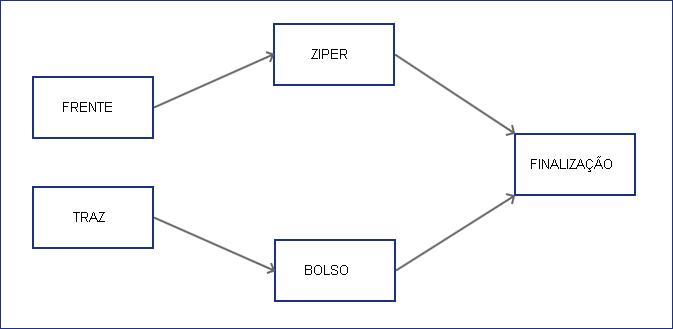
\includegraphics[scale=0.5]{./imagens/processo1.png}}
	\caption[Demonstração de um processo de fabricação de uma calça.]
	{Demonstração de um processo de fabricação de uma calça. \textbf{Fonte:}
	Desenvolvido pelos autores.}
	\label{fig:processo_fabricacao}
\end{figure}

\par  Uma questão importante que foi definida é que, independente da complexidade e tamanho do processo, este deve sempre começar 
com a atividade carimbo e finalizar com a atividade Finalização. Isso ocorre pois a finalização é sempre a última atividade 
de qualquer processo da fábrica e o carimbo é uma atividade simbólica que representa o fato de o dono da fábrica separar o 
material de costura. O tempo gasto e o custo desta separação não são contabilizados no algoritmo genético, somente o tempo de 
transporte dos materiais até as costureiras são considerados na distribuição, além disto esta atividade terá somente uma pessoa
trabalhando que, neste caso será o Marcelo, dono da fábrica, que é o responsável por este trabalho.

\par Para armazenar este processo e suas atividades no software, foram utilizadas tabelas do banco de dados, conforme mostra 
a Figura~\ref{fig:proc_fabri_db}.

\newpage

\begin{figure}[h!]
	\centerline{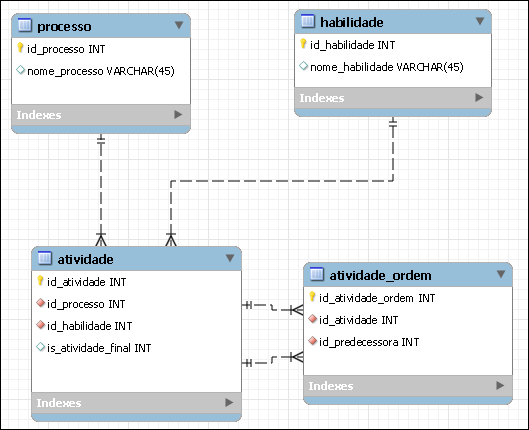
\includegraphics[scale=0.7]{./imagens/representacao_processo.png}}
	\caption[Modelo do processo de fabricação no banco de dados.]
	{Representação do processo de fabricação no banco de dados. \textbf{Fonte:}
	Desenvolvido pelos autores.}
	\label{fig:proc_fabri_db}
\end{figure}

\par A tabela \texttt{processo} tem como finalidade gerar um código único para representar 
cada processo de produção, cada processo representa um modelo, cada modelo
de calça possui um processo diferente que pode possuir diferentes atividades que
são representadas na tabela \texttt{atividade}, onde é feita a relação que define quais são as atividades de 
um processo,  além de conter quais são as habilidades necessárias para cada atividade, ou seja, cada registro desta 
tabela representa uma atividade do processo e qual habilidade é necessária para sua execução. O campo 
\texttt{is\_atividade\_final}, quando tem o valor 1, define que tal atividade
é a atividade Finalização. Esta \textit{flag} é importante no momento de calcular o tempo total de execução do
processo e será visto com mais detalhes posteriormente e, por fim, a tabela
\texttt{atividade\_ordem} é onde é feita a definição de ordem de execução das
atividades.

\par A Figura~\ref{fig:class_atividadeOrdem} demonstra as classes que representam o mapeamento da relação
entre a tabela \texttt{atividade} e \texttt{atividade\_ordem} para o Java.

\newpage

\begin{figure}[h!]
	\centerline{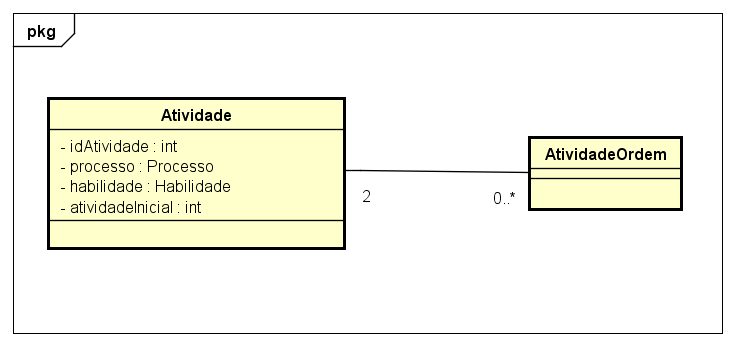
\includegraphics[scale=0.7]{./imagens/atividade_diagram.png}}
	\caption[Classes \texttt{Atividade} e \texttt{AtividadeOrdem}.]
	{Classes \texttt{Atividade} e \texttt{AtividadeOrdem}. \textbf{Fonte:}
	Desenvolvido pelos autores.}
	\label{fig:class_atividadeOrdem}
\end{figure} 

\par A classe \texttt{Atividade} pode ter zero ou vários objetos da classe
\texttt{AtividadeOrdem}.
Esta possui dois objetos da própria classe \texttt{Atividade}, um representando uma
atividade e outro representando a sua predecessora.

\par Considerando o processo de produção e o modelo de dados apresentados anteriormente, foi
desenvolvido um algoritmo genético para a solução do problema de otimização. Conforme já demonstrado 
no capítulo~\ref{quadro_teorico}, um algoritmo genético deve seguir uma ordem de execução conforme mostra
a Figura~\ref{fig:representacao_ags} (ver página 16).

\par O primeiro passo para a execução do algoritmo então foi o desenvolvimento de uma lógica para a criação
da população inicial de indivíduos.

\subsection {População inicial: Distribuição das atividades, Indivíduos e Cromossomos} \label{populacao_inicial_section}

\par Para um melhor entendimento dos conceitos a serem explanados, é necessário
conhecer, de forma básica, o fluxo de execução da aplicação. Como será visto na seção~\ref{interface_grafica_section}, o usuário irá iniciar a execução do algoritmo genético através de uma tela de distribuição de atividades, nesta tela ele deve informar o número de peças que deseja produzir, a quantidade de peças que cada lote deve possuir e uma data de início das atividades. Através da data de início e a data de entrega, informada no cadastro do processo, o controlador da tela calcula o prazo de entrega e o número total de lotes e chama o serviço de gerenciamento da execução do AG, passando o número de lote, o número de peças por lote e o prazo de entrega a ser considerado durante a distribuição. Tal serviço, por sua vez, configura os parâmetros do algoritmo genético e da início a execução deste. A Figura~\ref{fig:fluxo_basico} ilustra o fluxo básico de execução da aplicação.

\begin{figure}[h!]
	\centerline{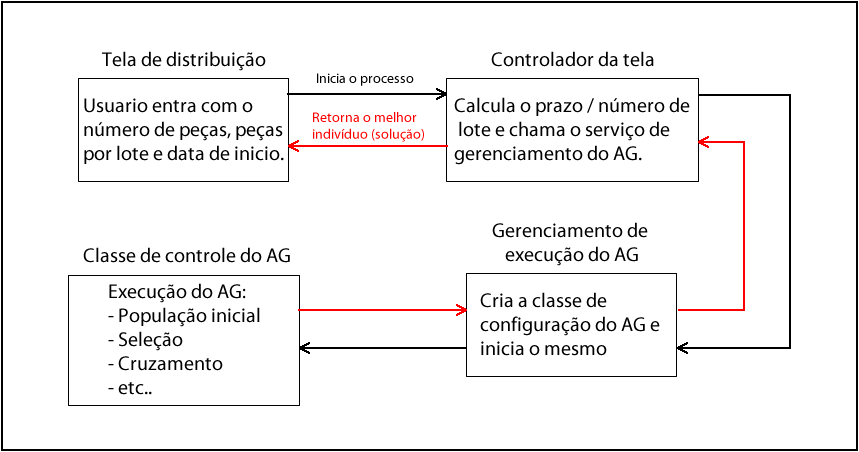
\includegraphics[scale=0.5]{./imagens/fluxo_basico.png}}
	\caption[Fluxo básico de execução.]
	{Fluxo básico de execução. \textbf{Fonte:} Desenvolvido pelos autores.}
	\label{fig:fluxo_basico}
\end{figure}

\par Conforme ilustrado na Figura~\ref{fig:fluxo_basico}, o processo de criação da população inicial assim como o processo de seleção, 
cruzamento e mutação e a chamada da função de avaliação de cada indivíduo, ocorre dentro de uma classe de controle,
ou seja, esta classe faz a orquestração de toda a execução do AG. Tal classe é denominada \texttt{GAController} e
pertence ao \textit{Framework} explanado anteriormente, na seção~\ref{framework_section}.

\par A classe criada para o gerenciamento da execução do algoritmo genético é denominada \texttt{GeneticAlgorithmManagement} e, conforme demonstrado na Figura~\ref{fig:fluxo_basico}, esta é instanciada pelo controlador da tela de distribuição de atividades. Tal classe possui 
um único método denominado \texttt{iniciarDistribuicao()} e recebe neste os dados informados pelo usuário, além disto, neste
método, é criado um objeto de \texttt{ProcessoModel}, que herda da classe \texttt{GAModel} do \textit{framework}, e, neste, são 
definidos os parâmetros a serem usados pelo algoritmo genético, além disso, os dados informados pelo usuário também são definidos 
neste objeto pois são utilizados pela regra de negócio seguida na execução do algoritmo. O Código~\ref{list:iniciarDistribuicao} 
demonstra o método \texttt{iniciarDistribuicao()}.


\begin{lstlisting} [style=custom_Java,caption={[Método \texttt{iniciarDistribuicao()} da classe \texttt{GeneticAlgorithm\-Management} ]
{Método \texttt{iniciarDistribuicao()} da classe \texttt{GeneticAlgorithmManagement}. \textbf{Fonte:}
Elaborado pelos autores.}}, label=list:iniciarDistribuicao]

public ProcessoIndividual iniciarDistribuicao(
			int numeroLote,BigDecimal prazEmSegundos,  
			int pecasPorLote,int idProcesso){

		EntityManager manager = ConFactory.getConn(); 
		
		ProcessoModel model = new ProcessoModel(manager,idProcesso);
		model.setNumeroLote(numeroLote);
		model.setPecasPorLote(pecasPorLote);
		model.setPrazoEmSegundos(prazEmSegundos);
		model.setGenerationQuantity(10000);
		model.setPopulationSize(80);
		model.setElitism(true);
		model.setSelectionType(GAModel.SelectionType.CLASSIFICATION);
		model.setCrossType(CrossType.PERMUTATION);
		model.setForeignIndividualRate(0.3f);
		model.setMutation(GAModel.MutationType.PERMUTATION);
		model.setMutationRate(0.05f);
		model.setMutationQuantity(1);

		GAController controller = new GAController(model);
		return (ProcessoIndividual) controller.execute();
}


\end{lstlisting}

\par Tal método retorna um objeto do tipo \texttt{ProcessoIndividual} para o controlador da tela de distribuição, este é o melhor indivíduo encontrado, ou seja, a melhor solução encontrada. Tal solução será então apresentada ao usuário conforme mostra a Figura~\ref{fig:fluxo_basico}.

\par A classe \texttt{ProcessoModel}, ao ser instanciada, recebe em seu construtor uma conexão para o 
banco de dados e o \texttt{ID} do processo a qual será executado o algoritmo, tal construtor então chama o método
\texttt{getInformacoesCostureiras()} que tem por finalidade buscar no banco de dados todas as atividades do processo em questão, 
buscar todas as costureiras que tem a habilidade de fazer cada uma destas e criar um \texttt{HashMap} que possui como chave o 
\texttt{ID} da atividade e como valor uma lista de \texttt{CostureiraHabilidade}, feito isto o método também recupera  a 
atividade final (finalização), conforme demonstra o Código~\ref{list:getInformacoesCostureiras}.


\begin{lstlisting} [style=custom_Java,caption={[Método \texttt{getInformacoesCostureiras()}]
{Método \texttt{getInformacoesCostureiras()}. \textbf{Fonte:}
Elaborado pelos autores.}}, label=list:getInformacoesCostureiras]

public void getInformacoesCostureiras() {
	List<CostureiraHabilidade> costureirasHabilidades = null;
	
	if (atividadesCostureiras != null && atividadesProcesso != null){
	   atividadesCostureiras.clear();
	   atividadesProcesso.clear();
	}
	
	atividadesCostureiras = 
	   new HashMap<Integer, List<CostureiraHabilidade>>();
	
	atividadesProcesso = 
	   atividadeDao.listAtividadesByProcesso(processo);
	
	/* Montar um MAP tendo como chave cada atividade do processo 
	   e a lista de costureiras que tenham a habilidade relacionada.*/
	for (Atividade atividade : atividadesProcesso) {
		
		costureirasHabilidades = 
		   cdao.getCostureirasByHabilidade
		      (atividade.getHabilidade().getIdHabilidade());
		
		atividadesCostureiras.put
		   (atividade.getIdAtividade(),costureirasHabilidades);
		
		if (atividade.isAtividadeFinal()) atividadeFinal = atividade;
	}
}

\end{lstlisting}

\par Então, de acordo com o Código~\ref{list:iniciarDistribuicao}, após a definição dos parâmetros, é criado um novo objeto de \texttt{GAController} passando-se o 
objeto da classe \texttt{ProcessoModel} com todos os parâmetros do algoritmo genético, os dados do usuário e 
informações de atividades e costureiras do processo em questão e então  o método \texttt{execute()} é chamado, dando-se início  
à execução do algoritmo genético. A primeira coisa a ser feita, neste método, é a criação da população inicial de indivíduos realizada a partir do método \texttt{createInitialPopulation()} declarado de forma abstrata na classe \texttt{GAModel} e implementado pela classe 
\texttt{ProcessoModel}. Tal método basicamente executa um \texttt{for} de 0 até o tamanho da população (atributo 
\texttt{populationSize}) e assim para cada iteração é criado um objeto de \texttt{ProcessoIndividual} passando a 
\texttt{atividadeFinal}, o \texttt{map} que contém as atividades e suas costureiras (\texttt{atividadesCostureiras}) criados 
pelo método \texttt{getInformacoesCostureiras()}, além dos atributos \texttt{numeroLote}, \texttt{pecasPorLote} e
\texttt{prazoEmSegundos}, conforme mostra o Código~\ref{list:createInitialPopulation}.


\begin{lstlisting} [style=custom_Java,caption={[Método \texttt{createInitialPopulation()}]
{Método \texttt{createInitialPopulation()}. \textbf{Fonte:} Elaborado pelos autores.}}, label=list:createInitialPopulation]

@Override
	public void createInitialPopulation() {
		for (int i = 0; i < getPopulationSize(); i++) {
			population.add
			   (new ProcessoIndividual
			       (atividadeFinal, prazoEmSegundos, atividadesCostureiras,
			        this.numeroLote, this.pecasPorLote));
	}
}

\end{lstlisting}

\par Quando se cria um novo indivíduo, a partir da instanciação de um novo objeto de \texttt{ProcessoIndividual},
acontece então, no construtor da classe, a distribuição das atividades de forma a representar uma solução para o problema.
Esta distribuição foi realizada considerando que o total de
peças a ser produzido deveria ser dividido em lotes e então, em cada atividade,
este número de lote deveria ser distribuído entre as costureiras que possuíssem a habilidade em questão. Por exemplo: se a quantidade total de peças de uma ordem de produção for 500,
primeiramente deve-se definir qual será o número de peças por lote, neste caso, se for definido que cada lote  
deverá ter 50 peças, então o resultado final será 500/50 ou seja 10 lotes contendo 50 calças cada um. 

\par Neste sentido, seguindo o exemplo apresentado  na Figura~\ref{fig:processo_fabricacao}, a distribuição deverá ser feita de forma que, para cada atividade do processo, seja 
distribuído o trabalho de 10 lotes, ou seja, o material para a confecção de 10 lotes deve ser enviado para as costureiras
que irão fazer a parte da frente e posteriormente estas enviam os 10 lotes para as costureiras que fazem a finalização.

\par Com base nesses requisitos, para a realização de tal distribuição, inicialmente, o algoritmo irá distribuir, 
de forma aleatória, o número de lotes definido entre as costureiras de cada atividade,
conforme mostra a Figura~\ref{fig:distribuicao_lotes_costureiras}.



\begin{figure}[h!]
	\centerline{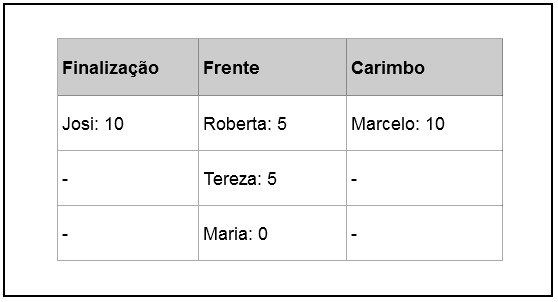
\includegraphics[scale=0.5]{./imagens/distribuicao_exemplo.png}}
	\caption[Exemplo de distribuição aleatória de lotes para as costureiras.]
	{Exemplo de distribuição aleatória de lotes para as costureiras.
	\textbf{Fonte:} Desenvolvido pelos autores.}
	\label{fig:distribuicao_lotes_costureiras}
\end{figure}

\par Uma costureira pode não receber lotes, isso permite que a decisão de
quem vai participar ou não também fique por conta do algoritmo.

\par Como já explanado no quadro teórico, a estrutura do algoritmo genético é composta
por populações que são formadas por indivíduos, que por sua vez são formados por cromossomos.
Cada indivíduo representa uma solução e cada cromossomo do indivíduo representa uma de suas características. 
Assim, então, é gerada uma população inicial de indivíduos e, a partir desta, um
processo de cruzamento e mutação é iniciado a fim de que possam ser gerados
novos indivíduos que representem soluções ainda melhores que seus antecessores.

\par Neste sentido, para o desenvolvimento do algoritmo de distribuição de
lotes, o processo de definição de indivíduo e cromossomo foi o primeiro passo do desenvolvimento da aplicação. Isso se
deve ao fato de que estes elementos compõe a parte crucial para que se
possa definir a lógica a ser seguida para a definição da população inicial, o
tipo de cruzamento, a função de avaliação, etc.

\par Neste caso, cada indivíduo da população irá representar uma forma de
distribuir as atividades e a quantidade de lotes distribuídos a determinada
costureira em uma determinada atividade irá representar um cromossomo. 
Tomando como base o exemplo da Figura~\ref{fig:distribuicao_lotes_costureiras},
o quadro, como um todo, representa o indivíduo e cada distribuição, como por exemplo a Roberta, que recebeu 5 
lotes para confeccionar a frente, representa um cromossomo.

\par Para fazer esta representação em Java, primeiramente foi criado uma classe denominada \texttt{ProcessoChromosome} que é
representada na Figura~\ref{fig:class_processoChromosome}:

\begin{figure}[h!]
	\centerline{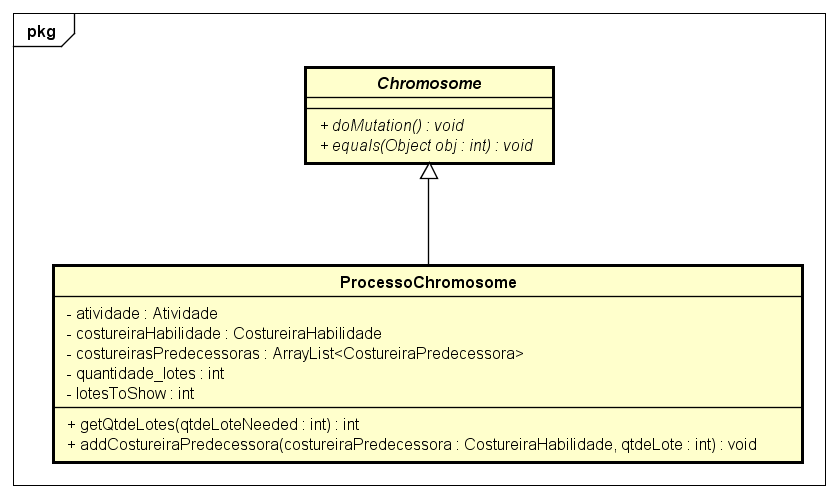
\includegraphics[scale=0.5]{./imagens/processo_chromosome_diagram.png}}
	\caption[Classe \texttt{ProcessoChromosome}.]
	{Classe \texttt{ProcessoChromosome}. \textbf{Fonte:} Desenvolvido pelos
	autores.}
	\label{fig:class_processoChromosome}
\end{figure}


\par A classe \texttt{ProcessoChromosome} herda de \texttt{Chromosome} do
\textit{framework} descrito na Figura ~\ref{fig:class_processoChromosome}. Por
enquanto, é necessário compreender apenas os atributos \texttt{atividade}, \texttt{costureiraHabi\-lidade} e
\texttt{quantidade\_lotes}, que recebem seus valores pelo construtor, os
demais atributos e métodos são utilizados pela função de avaliação e serão explicados mais adiante. 
O atributo \texttt{atividade} representa o \texttt{ID} da
atividade a qual se está atribuindo a costureira e a
quantidade de lotes, este atributo será passado na criação de cada cromossomo
sempre que for necessário se criar um novo indivíduo. O atributo \texttt{costureiraHabilidade} 
é do tipo \texttt{CostureiraHabilidade}, que representa o mapeamento da tabela \texttt{costureira\_habilidade} do banco de dados onde 
é feita a relação entre quais habilidades cada costureira possui além do tempo e o preço de cada uma para 
fazer uma peça de uma determinada parte da calça, além disto, na tabela \texttt{costureira}, foram definidos os campos \texttt{posicaoX} e \texttt{posicaoY} que definem a localização da costureira, conforme demonstra a Figura~\ref{fig:dados_costureiras}. Estes valores serão utilizados posteriormente para calcular a distância entre duas costureiras, 

\newpage

\begin{figure}[h!]
	\centerline{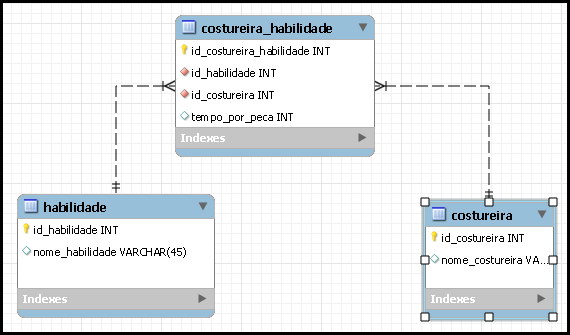
\includegraphics[scale=0.6]{./imagens/costureira_habilidade_tabela.png}}
	\caption[Armazenamento de dados das costureiras.]
	{Armazenamento de dados das costureiras. \textbf{Fonte:} Desenvolvido pelos
	autores.}
	\label{fig:dados_costureiras}
\end{figure}


\par A classe \texttt{CostureiraHabilidade}, conforme ilustra a Figura~\ref{fig:class_costureiraHabilidade}, por sua vez, possui o atributo habilidade, outro que
representa a costureira, além de dois atributos que representam o tempo de produção e o custo 
de cada costureira para confeccionar uma peça de uma determinada parte. Fez-se
necessário ter um atributo da classe \texttt{CostureiraHabilidade} ao invés de simplesmente ter um objeto do tipo Costureira, pois, 
na função de avaliação, como será visto mais adiante, é necessário ter tempo gasto e o preço de cada costureira para se fazer uma peça 
e estas informações podem variar para uma mesma costureira dependendo de suas habilidades.


\begin{figure}[h!]
	\centerline{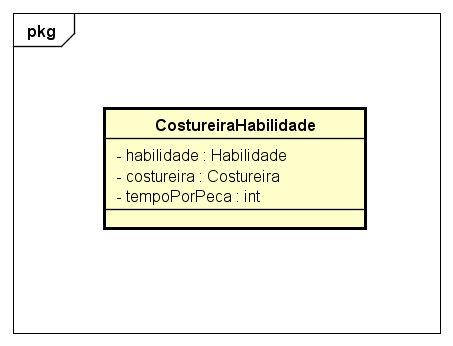
\includegraphics[scale=0.5]{./imagens/costureiraHabilidade_class.png}}
	\caption[Classe \texttt{CostureiraHabilidade}.]
	{Classe \texttt{CostureiraHabilidade}. \textbf{Fonte:} Desenvolvido pelos
	autores.}
	\label{fig:class_costureiraHabilidade}
\end{figure}

\par Assim, para representar cada característica da solução, tomando como
exemplo a Figura~\ref{fig:distribuicao_lotes_costureiras}, o fato de Roberta
fazer 5 lotes da parte da frente é representado na implementação do código criando se um objeto da classe \texttt{ProcessoChromosome} passando no construtor o \texttt{id} da atividade frente, um objeto de
\texttt{costureiraHabilidade}, cujo atributo \texttt{costureira} represente a
Roberta, o atributo \texttt{habilidade} que representa a habilidade em questão e a
quantidade de lotes que Roberta deverá confeccionar, que seria, neste caso, cinco.

\par A representação do indivíduo foi feita criando-se a classe \texttt{ProcessoIndividual} 
como demonstra a Figura~\ref{fig:class_processoIndividual}:


\begin{figure}[h!]
	\centerline{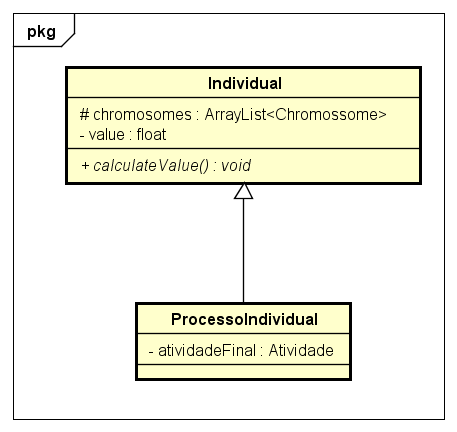
\includegraphics[scale=0.7]{./imagens/class_individual.png}}
	\caption[Classe \texttt{ProcessoIndividual}.]
	{Classe \texttt{ProcessoIndividual}. \textbf{Fonte:} Desenvolvido pelos
	autores.}
	\label{fig:class_processoIndividual}
\end{figure}

\par A classe \texttt{ProcessoIndividual} herda da classe \texttt{Individual} do
\textit{framework}, e por isso, esta passa a ter um \texttt{ArrayList} com
objetos do tipo \texttt{Chromosome}. Neste caso, como a classe \texttt{ProcessoChromosome} herda de \texttt{Chromosome}, 
este \texttt{ArrayList} terá objetos do tipo \texttt{ProcessoChromosome}.

\par A criação dos cromossomos que irão compor o indivíduo é feita através do construtor da classe 
\texttt{ProcessoIndividual} e, é neste ponto, que os lotes são distribuídos as costureiras de cada atividade.
O \texttt{construtor} da classe \texttt{ProcessoIndividual} recebe como
parâmetro um objeto representando a atividade final, que será utilizado pela função de avaliação mais adiante, e um \texttt{HashMap} que possui como chave o
\texttt{ID} de uma atividade e uma lista do  tipo \texttt{CostureiraHabilidade} contendo as costureiras e suas respectivas informações de tempo e preço para se fazer tal atividade.

\par Com base neste \texttt{HashMap} então é feita a criação dos cromossomos do indivíduo.
Em um primeiro momento, a distribuição de tarefas entre as costureiras seria feita em forma 
de porcentagem, ou seja, o algoritmo distribuiria uma porcentagem aleatória para cada costureira de 
uma determinada atividade, desta forma a distribuição seria feita conforme demonstra o código~\ref{list:distribuicaoPorcentagem}.

\begin{lstlisting} [style=custom_Java,caption={[Criação de cromossomos (Primeira Abordagem)]
{Criação de cromossomos (Primeira Abordagem). \textbf{Fonte:} Elaborado pelos autores.}}, label=list:distribuicaoPorcentagem] 	
	package edu.univas.edu.tcc.ga_code;
	
	import java.util.ArrayList;
	
	public class ProcessoIndividual extends Individual {
		
		public Atividade atividadeFinal;
		
		public ProcessoIndividual(Atividade atividadeInicial,
			Map<Integer, List<CostureiraHabilidade>> atividadesCostureiras){
		
			chromosomes = new ArrayList<Chromosome>();
			this.atividadeFinal = atividadeInicial;
			
			for(Integer key: atividadesCostureiras.keySet()){
			   for(CostureiraHabilidade costureira : 
				   atividadesCostureiras.get(key)){
				
				   Float porcentagem = (float) (Math.random() *1);
				   chromosomes.add(new ProcessoChromosome(key, 
					   costureira, porcentagem));
				}
			}
		}
	}

\end{lstlisting}
 
\par Feita a distribuição da porcentagem, antes de fazer o cálculo do indivíduo, seria então realizado 
um cálculo de normalização para que se pudesse encontrar o número de lotes a ser
produzido por cada costureira em cada atividade. Tomando como exemplo a Figura~\ref{fig:distribuicao_porcentagem}, este cálculo seria feito da seguinte forma:

\begin{figure}[h!]
	\centerline{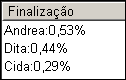
\includegraphics[scale=1.0]{./imagens/distribuicao_porcentagem.png}}
	\caption[Distribuição em porcentagem.]
	{Distribuição em porcentagem. \textbf{Fonte:} Desenvolvido pelos autores.}
	\label{fig:distribuicao_porcentagem}
\end{figure}

\begin{itemize}
	\item Primeiramente deveria ser feito a soma de todas as porcentagens distribuídas, logo: 
	\par \texttt{0,53 + 0,44 + 0,29 = 1,26};
	
	\item o segundo passo seria calcular quanto cada porcentagem equivale dentro do total, neste 
	sentido o cálculo, já fazendo o arredondamento, seria: 
	\par \texttt{0,53 / 1,26 = 0,42 | 0,44 / 1,26 = 0,35 | 0,29 / 1,26 = 0,23}
	\par Logo, neste caso a Andrea seria responsável por 42\%, a Dita por 35\% e a Cida por 23\%;
	
	\item Assim, seria feito um cálculo com regra de 3 com o número total de peças. Supondo que o 
	 valor total fosse 500, logo:
	
	\par \texttt{(500 * 42) / 100 = 210 | (500 * 35) / 100 = 175 | (500 * 23) / 100 = 115}
	
	\par Neste caso então, a Andrea deveria produzir 210 peças, a Dita 175 e a Cida 115 peças;
	
	\item Por fim deveria ser feito uma divisão dos número de peças de cada costureira pela quantidade
     de peças por lote, que neste caso poderia ser 50, então realizando o cálculo já com arrendondamento:
     \par \texttt{210 / 50 = 4 | 175 / 50 = 4 | 115 / 50 = 2}
     
     \par Assim, a Andrea produziria 4 lotes, a Dita 4 e a Cida 2, dando o total
     dos 10 lotes a serem produzidos para a atividade de finalização.
	
\end{itemize}
 
 \par Os passos acima para distribuição de atividades seriam então repetidos
 para cada atividade chave do \texttt{HashMap} realizando tal distribuição para cada costureira da lista de 
 costureiras de cada atividade. No momento de fazer o último cálculo, foi feito
 um arredondamento, com isso se uma costureira tivesse tido uma porcentagem muito pequena, o valor de lotes para
 esta seria 0, eliminando-a assim da distribuição.
 
 \par Todavia verificou-se que, distribuindo desta forma, em alguns casos, o total de lotes por atividade não era distribuído
 de forma correta. Devido ao arredondamento, as vezes uma atividade ficava com lotes a menos ou lotes a mais do que o total
 definido, o que poderia causar erros no cálculo final. Além disso, no momento de definir como seria o cruzamento 
 surgiu uma questão importante que é o fato de que todas as vezes que fosse criado um indivíduo a partir de outros, deveria
 ser realizado o cálculo de normalização, e com isso a distribuição de lotes no novo indivíduo poderia ficar completamente
 diferente de seus pais, resultando assim na quebra do paradigma de algoritmos genéticos que descreve que os indivíduos filhos
 devem ser formados pela mesclagem das características dos pais. 


\par Buscou-se então uma outra alternativa para se realizar a distribuição dos lotes e definiu-se que, ao invés de distribuir
a porcentagem, a distribuição já deveria ser feita a nível de lote sendo esta também realizada de forma aleatória. Os parâmetros
do \texttt{construtor} da classe \texttt{ProcessoIndividuo} permaneceram da mesma forma, alternando somente a forma com que 
os lotes são distribuídos entre as costureiras em cada atividade conforme mostra
o Código~\ref{fig:distribuicaoDiretamente}.


\begin{lstlisting} [style=custom_Java,caption={[Distribuição em lotes diretamente.]
{Distribuição em lotes diretamente. \textbf{Fonte:} Elaborado pelos autores.}}, label=fig:distribuicaoDiretamente] 	
public ProcessoIndividual(Atividade atividadeFinal,
	BigDecimal prazoEmSegundos, 
	Map<Integer, List<CostureiraHabilidade>> atividadesCostureiras, 
	int numeroLote, int pecasPorLote){
	
	chromosomes = new ArrayList<Chromosome>();
	Map<Integer, ProcessoChromosome> chromossomosMap = 
		new HashMap<Integer, ProcessoChromosome>();
	
	this.atividadeFinal = atividadeFinal;
	this.numeroLote = numeroLote;
	this.pecasPorLote = pecasPorLote;
	this.prazo = prazoEmSegundos;
	
	boolean distribuiuPorTodasCostureiras = false;
	
	int qtdeLote = 0;
	int cont = 0;
	
	for (Integer key : atividadesCostureiras.keySet()) {
		qtdeLote = numeroLote;
		cont = 0;
		int loteCostureira = 0;
		distribuiuPorTodasCostureiras = false;
		
		while (true){
			/* Verificou-se que quando a qtdeLote era 1 o valor
			   sorteado nunca era zero usando o Math.random com 
			   CAST para INT */
			if(qtdeLote == 1){
				loteCostureira  = Math.round((float) Math.random() * 1);
			}else{
				loteCostureira = (int) (Math.random() * qtdeLote);
			}
		
			CostureiraHabilidade costureiraHabilidade = 
				atividadesCostureiras.get(key).get(cont);
				
			ProcessoChromosome intermediario = 
				chromossomosMap.get(costureiraHabilidade.getIdCostureiraHabilidade());
				
			if(intermediario == null){
				ProcessoChromosome pc = new ProcessoChromosome
					(key, costureiraHabilidade,loteCostureira); 
					
				chromossomosMap.put
					(costureiraHabilidade.getIdCostureiraHabilidade(), pc);
					
				chromosomes.add(pc);
			}else{
				int oldValue = intermediario.getQuantidade_lotes();
				int newValue = oldValue + loteCostureira;
				intermediario.setQuantidade_lotes(newValue);
				intermediario.setLotesToShow(newValue);
			}
			
			if (cont == atividadesCostureiras.get(key).size() - 1) {
				cont = -1;
				distribuiuPorTodasCostureiras = true;
			} 
	
			qtdeLote -= loteCostureira;
			
			if(qtdeLote == 0 && distribuiuPorTodasCostureiras){
				break;
			}
			cont++;
		}
	}
}

\end{lstlisting}
 
\par Conforme descrito no Código~\ref{fig:distribuicaoDiretamente}, é feita uma
iteração no \texttt{HashMap} e, para cada atividade, é feita a distribuição dos lotes para
as costureiras desta lista. O algoritmo então atribui a cada costureira um valor
que pode variar de 0 até \texttt{qtdeLote}. Assim são criados objetos da classe \texttt{ProcessoChromosome} 
e colocados na lista de cromossomos do indivíduo. Após a criação de cada cromossomo, a quantidade de
lotes é subtraída pelo valor atribuído ao cromossomo recém criado.
Se a iteração passar por todas as costureiras da lista, o contador é reiniciado e então, se ao final sobrar 
lotes a serem distribuídos, a distribuição recomeça na primeira costureira, acrescentando assim seu 
número de lotes de acordo com o novo valor sorteado. A iteração termina quando não há mais lotes a serem 
distribuídos e a execução já passou por todas as costureiras. Em uma primeira versão, quando a execução chegava
ao final da lista de costureiras e ainda existiam lotes a serem distribuídos, este restante de lotes era atribuído
à última costureira, porém verificou-se, que desta forma, o algoritmo tendia a nunca distribuir zero lotes à última
costureira, o que causou resultados ineficazes na distribuição. Alterando para esta forma, a distribuição  passou a 
ser feita de maneira totalmente uniforme deixando o resultado coerente.
Como é possível perceber, neste processo uma costureira pode receber aleatoriamente o valor 0, o que irá resultar na 
sua eliminação do processo da mesma forma que iria ocorrer na primeira abordagem. Por fim, após a finalização do primeiro
\texttt{for} um novo indivíduo terá sido criado, semelhante ao quadro
apresentado na Figura~\ref{fig:distribuicao_lotes_costureiras}.

\par Concluindo, a distribuição das atividades ocorre todas as vezes que se cria um novo indivíduo.
Tais indivíduos podem ser criados no processo de criação da população inicial, na criação de 
indivíduos estrangeiros e no processo de cruzamento, como será descrito nas próximas subseções,
ressaltando porém que no processo de cruzamento, os cromossomos do indivíduo é a mistura dos cromossomos dos pais,
já criados anteriormente, e portanto há também um construtor na classe \texttt{ProcessoIndividual} que recebe uma lista de 
cromossomos para se criar um novo indivíduo. Este processo será demonstrado na seção que descreve o cruzamento.


\subsection{Função de avaliação}

\par Após a criação da população inicial, esta é então submetida a um processo
de avaliação. Assim é feita uma iteração sobre a lista de indivíduos e para cada um é chamado então o seu método 
\texttt{calculateValue()}. Tal método é declarado de forma abstrata na classe mãe
\texttt{Individual} e implementado na classe \texttt{ProcessoIndividual}.

\par Assim como já foi visto anteriormente, cada costureira sabe fazer uma ou
mais partes da calça e gasta um determinado tempo, medido em segundos, além de cobrar um valor 
para se produzir cada peça, que varia de  acordo com a habilidade, além disto, existe um 
tempo de transporte entre cada costureira que é medido através da distância euclidiana, 
ou seja, cada costureira recebe um valor X e Y que representam sua localização, e então 
para se calcular a distância entre duas costureiras, os valores X e Y de cada uma delas
são inseridos como variáveis na fórmula euclidiana obtendo-se assim
a distância entre elas. A Figura~\ref{fig:demonstracao_costureiras_habilidades} demonstra 
exemplo de dados a serem considerados para o cálculo do valor do indivíduo.


\begin{figure}[h!]
	\centerline{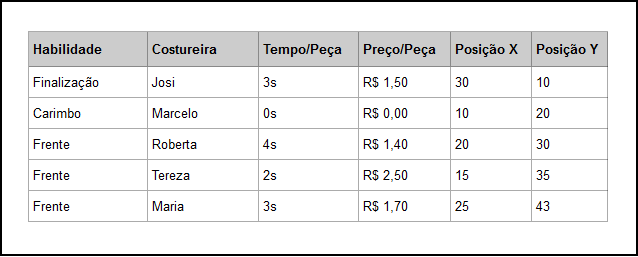
\includegraphics[scale=0.5]{./imagens/tempo_habilidade_3.PNG}}
	\caption[Demonstração de costureiras e habilidades.]
	{Demonstração de costureiras e habilidades. \textbf{Fonte:} Desenvolvido pelos
	autores.}
	\label{fig:demonstracao_costureiras_habilidades}
\end{figure}

\par Com base nestes dados é realizado um cálculo a fim de se encontrar o custo e o tempo total de fabricação do número de peças
desejado e, ao fim, um valor de tempo e custo de produção será atribuído ao indivíduo. É importante ressaltar que a função de avaliação tem a responsabilidade apenas de definir o valor do indivíduo, que neste caso é o tempo e o custo de produção, a escolha dos indivíduos mais aptos será feita posteriormente no processo de classificação.

\par Para o desenvolvimento do cálculo do tempo de produção, foi necessário construir uma estrutura para representar a 
questão da ordem de precedência entre as atividades. Tal estrutura, conforme é demonstrado na Figura~\ref{fig:montagem_node}, 
deveria possuir nós representando cada atividade, as costureiras que trabalham em cada atividade e o número de lotes atribuídos a 
cada uma aleatoriamente pelo algoritmo.

\newpage

\begin{figure}[h!]
	\centerline{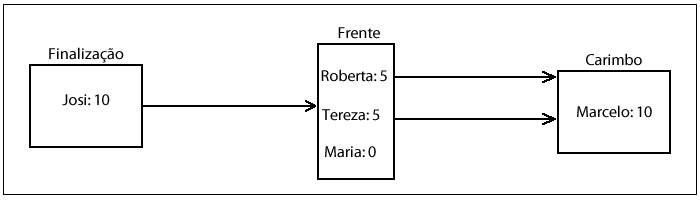
\includegraphics[scale=1.1]{./imagens/montagem_node.png}}
	\caption[Estrutura de representação da ordem de precedência.]
	{Estrutura de representação da ordem de precedência. \textbf{Fonte:}
	Desenvolvido pelos autores.}
	\label{fig:montagem_node}
\end{figure}


\par Como foi visto na seção 3.4.2, cada indivíduo possui uma lista de
cromossomos, e cada cromossomo, por sua vez, representa a alocação de uma
costureira, contendo os lotes que esta deve produzir para uma determinada atividade.
Desta forma, para calcular o custo total de produção, foi realizada uma iteração 
na lista de cromossomos do indivíduo somando o preço total de confecção dos lotes
que cada costureira recebeu aleatoriamente pelo algoritmo conforme mostra o Código~\ref{list:metodoCalculateValue}.

\par Para o cálculo do tempo de produção, definiu-se então que tal lista de cromossomos deveria ser
dividida de forma que se pudesse agrupar os cromossomos por atividade estabelecendo assim a relação 
demonstrada na Figura~\ref{fig:montagem_node}, para, que
por fim, o cálculo pudesse ser realizado.
Para isso, conforme demonstrado no Código~\ref{list:metodoCalculateValue}, primeiramente, a lista de 
cromossomos foi distribuída em um \texttt{HashMap} denominado \texttt{atividadeCromossomos}, contendo 
como chave a atividade e como valor a lista de cromossomos para a respectiva atividade e foi criado uma 
classe denominada \texttt{Node}, sendo esta a responsável por criar a estrutura
mostrada na Figura~\ref{fig:montagem_node}.

\par O método \texttt{calculateValue()}, após agrupar os cromossomos por atividade, 
 instancia um objeto da classe \texttt{Node} passando a atividade final e o número de 
 peças por lote recebidos na criação do indivíduo, conforme descrito na seção~\ref{populacao_inicial_section}, e o \texttt{MAP} 
 \texttt{atividadeCromossomos} conforme mostra o Código~\ref{list:metodoCalculateValue}.


\begin{lstlisting} [style=custom_Java,caption={[Método \texttt{calculateValue()}]
{Método \texttt{calculateValue()}. \textbf{Fonte:} Elaborado pelos autores.}}, label=list:metodoCalculateValue]
	public void calculateValue() {
		Map<Integer, List<Chromosome>> atividadeCromossomos 
			= new HashMap<Integer, List<Chromosome>>();
		
		Integer lastAtividade = null;
		float custoTotal = 0;
		int totalPecasAProduzir = 0;
		List<Chromosome> cromossomos = null;
		
		/*Calcular o custo total*/
		for(Chromosome chromosomeCusto : chromosomes){
			totalPecasAProduzir = 0;
			ProcessoChromosome processoChromossome = 
				(ProcessoChromosome) chromosomeCusto;
				
			totalPecasAProduzir = 
				processoChromossome.getLotesToShow() * this.pecasPorLote;
				
			custoTotal += totalPecasAProduzir * 
				processoChromossome.getCostureiraHabilidade()
					.getPrecoPorPeca();
		}
		
		for (Chromosome chromosome : chromosomes) {
		ProcessoChromosome processoChromossome = 
			(ProcessoChromosome) chromosome;
		
			if (lastAtividade == null || lastAtividade != 
				processoChromossome.getAtividade()) {
				
				cromossomos = new ArrayList<Chromosome>();
				
				atividadeCromossomos.put
					(processoChromossome.getAtividade(),cromossomos);
				lastAtividade = processoChromossome.getAtividade();
			}
			cromossomos.add(processoChromossome);
		}
		node = new Node(
			atividadeFinal, atividadeCromossomos,this.pecasPorLote);
		
		setCusto(custoTotal);
		
		
		/*So deve-se calcular o valor do individuo se 
		  ele nao foi calculado ainda porque uma vez calculado 
		  o valor o numero de lotes no objeto cromossomo foi 
		  decrementado */
		if (this.getTempoTotalProducao() == 0) {
			this.setTempoTotalProducao(node.getTempoTotal());
			setRootNode(node);
		}
	}

\end{lstlisting}


\par A estrutura da classe \texttt{Node} foi realizada de forma a produzir objetos de si mesma de forma recursiva, assim 
cada vez que esta é instanciada, é como se criasse um nó daqueles mostrados na Figura~\ref{fig:montagem_node}. Assim,
quando o método \texttt{calculateValue()} instancia um objeto \texttt{Node}, outros nós são criados a partir do construtor
de forma recursiva, e então toda estrutura, como foi ilustrada na Figura~\ref{fig:montagem_node}, será criada. 
O Código~\ref{list:classeNode} mostra a construção de um objeto \texttt{Node}.

\begin{lstlisting} [style=custom_Java,caption={[Construtor da classe \texttt{Node}]
{Construtor da classe \texttt{Node}. \textbf{Fonte:} Elaborado pelos autores.}}, label=list:classeNode]
	public Node(Atividade atividade,Map<Integer,List<Chromosome>>
		 atividadeCromossomos, int pecasPorLote){
		
		this.atividade = atividade;
		this.pecasPorLote = pecasPorLote;
		cromossomos = atividadeCromossomos.
			get(atividade.getIdAtividade());
			
		Atividade atividadePredecessora = null;
		
		for(AtividadeOrdem predecessora : 
			atividade.getAtividadeOrdemsForIdAtividade()){
			
			atividadePredecessora = 
				predecessora.getAtividadePredecessora();
		
			predecesoras.add(new Node(atividadePredecessora,
				atividadeCromossomos,pecasPorLote));
		}
	}
\end{lstlisting}

\par A classe \texttt{Node} recebe em seu construtor um objeto de \texttt{Atividade}, que na primeira vez em que o objeto for instanciado,
será a atividade final, o \texttt{MAP} com todos os cromossomos e o número de peças por lote, que será utilizado posteriormente.
O construtor então armazena as informações e pega do \texttt{MAP} somente os cromossomos relacionados à atividade recebida no construtor e, 
por fim, faz uma iteração na lista de atividades predecessoras de tal atividade e, recursivamente, cria novos nós, 
construindo assim, a estrutura demonstrada na Figura~\ref{fig:montagem_node}.

\par Como se pode ver no método \texttt{calculateValue()} no Código\ref{list:metodoCalculateValue}, após criar a estrutura de nós, é chamado o método \texttt{getTempoTotal()} do objeto \texttt{node}. Este método é responsável por iniciar a sequência lógica que 
faz o cálculo do tempo total a ser gasto pelo indivíduo, calculando o tempo gasto por 
cada costureira, definindo quem irá enviar peças para quem e calculando o tempo de transporte 
de cada envio, conforme demonstra o Código~\ref{list:codigo_metodo_get_valor_total} .

\begin{lstlisting} [style=custom_Java,caption={[Método \texttt{getValorTotal()}]{Método \texttt{getValorTotal()}. \textbf{Fonte:} Elaborado pelos autores.}}, label=list:codigo_metodo_get_valor_total] 	
	public long getTempoTotal(){
		long valor =  0;
		long maior = 0;
		
		for(Chromosome chromosome : cromossomos){
			ProcessoChromosome processoChromosome = 
				(ProcessoChromosome) chromosome;
		
			if(processoChromosome.getQuantidade_lotes() > 0){
				valor = getCromossomeValue(processoChromosome,
					processoChromosome.getQuantidade_lotes());
			}
	
			if(valor > maior){
				maior = valor;
			}
		}
		return maior;
	}

\end{lstlisting}


\par O método faz uma iteração na lista de cromossomos do nó da atividade final e irá chamar o método \texttt{getChromosomeValue()} passando 
cada cromossomo e o valor de seus lotes, e irá retornar o valor do maior cromossomo.

\par Tomando como base a Figura~\ref{fig:montagem_node}, para facilitar o
entendimento, o método \texttt{getChromosomeValue()} será chamado passando o cromossomo "Josi" e o inteiro 10 na quantidade de lotes. 
Este método é responsável por calcular o tempo gasto 
pela costureira para confeccionar os lotes atribuídos a ela. O tempo gasto pela
costureira é definido por \texttt{NLC * QPL * TP}, onde: \texttt{NLC} é o número
de lotes atribuídos para a costureira, \texttt{QPL} é a quantidade de peças por
lote e o \texttt{TP} é o tempo que a costureira gasta para fazer cada peça, 
porém este tempo também é influenciado pelo tempo que se é gasto para receber 
as partes dependentes, conforme demonstra o Código~\ref{list:codigo_metodo_get_cromossome_value}.


\begin{lstlisting} [style=custom_Java,caption={[Método \texttt{getCromossomeValue()}.]{Método \texttt{getCromossomeValue()}. \textbf{Fonte:} Elaborado pelos autores.}}, label=list:codigo_metodo_get_cromossome_value] 	

public long getCromossomeValue(ProcessoChromosome processoChromosome,
	int qtdeLote){
	
	long valor = 0;
	valor = qtdeLote * this.pecasPorLote *
		 processoChromosome.getCostureiraHabilidade().getTempoPorPeca();

	valor += getTempoRecebimentoPecas(processoChromosome,qtdeLote);
	return valor;
}

\end{lstlisting}

\par O método \texttt{getChromossomeValue()} chama então o método getTempoRecebimentoPecas(), passando o cromossomo Josi e 
o inteiro 10 como quantidade de lote. O método chamado tem a função de fazer uma busca nos nós predecessores buscando encontrar 
qual o tempo gasto para o recebimento das partes predecessoras da atividade e retornar o maior valor, 
conforme demonstra o Código~\ref{list:codigo_metodo_get_recebimento_pecas}.

\begin{lstlisting} [style=custom_Java,caption={[Método \texttt{getTempoRecebimentoPecas()}.]{Método \texttt{getTempoRecebimentoPecas()}. \textbf{Fonte:} Elaborado pelos autores.}}, label=list:codigo_metodo_get_recebimento_pecas] 	

	public long getTempoRecebimentoPecas(
		ProcessoChromosome processoChromosome, int qtdeLote){
		
		long valor = 0;
		long maior = 0;
		
		for(Node node : predecesoras){
			valor = node.getValueChromosomosPredecessores(
				processoChromosome, qtdeLote);
			
			if(valor > maior){
				maior = valor;
			}
		}
		return maior;
	}
}

\end{lstlisting}


\par Neste ponto começa então um processo recursivo, pois é chamado um método da
própria classe \texttt{Node}, só que de uma outra instância. O método chamado é o \texttt{getValueChromosomosPr\-edecessores()} 
passando o cromossomo Josi e o inteiro 10, como número de lotes. O código~\ref{list:codigo_metodo_getValueChromosomosPredecessores} 
mostra este método.


\begin{lstlisting} [style=custom_Java,caption={[Método \texttt{getValueChromosomosPredecessores()}.]
{Método \texttt{getValueChromosomosPredecessores()}. \textbf{Fonte:} Elaborado pelos autores.}}, label=list:codigo_metodo_getValueChromosomosPredecessores] 	

	public long getValueChromosomosPredecessores(
		ProcessoChromosome processoChromosome,int qtdeLote){
	
		int qtdeEachCromossome = 0;
		long valor = 0;
		long maior = 0;
		long distance = 0;
		
		for(Chromosome chromosome : cromossomos){
			ProcessoChromosome processoChromosomeBefore =
			   (ProcessoChromosome) chromosome;
			
			qtdeEachCromossome =
			   processoChromosomeBefore.getQtdeLotes(qtdeLote);
			
			if(qtdeEachCromossome > 0){
				qtdeLote -= qtdeEachCromossome;
				valor = getCromossomeValue(
					processoChromosomeBefore, qtdeEachCromossome);
					
				distance = calcularTempoEntreCostureiras(
					processoChromosome, processoChromosomeBefore);
				
				processoChromosome.addCostureiraPredecessora(
					processoChromosomeBefore.getCostureiraHabilidade(), 
					
				qtdeEachCromossome,distance,valor);
				
				valor += distance;
			}
			
			if(valor > maior){
				maior = valor;
			}
			
			if(qtdeLote == 0){
				break;
			}
		}
		return maior;
	}	
\end{lstlisting}

\par Tal método é responsável por iterar sobre a lista de cromossomos do nó anterior buscando de qual ou quais costureiras 
podem ser obtidos os lotes, retornando o maior valor. No exemplo da Figura~\ref{fig:ex_solicitaca_lotes}, a atividade anterior 
é a frente e a primeira costureira da lista é a Roberta, assim a Josi solicita 10 lotes da parte da frente para a Roberta, porém, 
neste caso, a Roberta confeccionou somente 5 lotes, então a Josi irá consumir os 5 lotes confeccionados.

\newpage

\begin{figure}[h!]
	\centerline{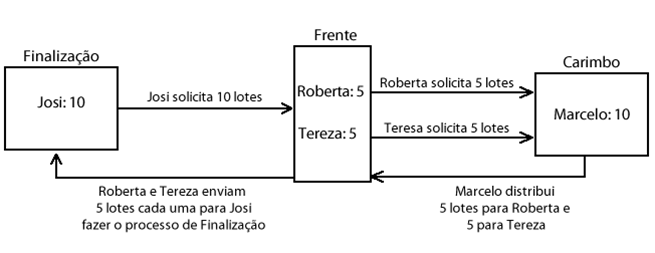
\includegraphics[scale=1.2]{./imagens/distribuicao_exemplo_apresentacao.png}}
	\caption[Exemplo de solicitação de lotes predecessores.]
	{Exemplo de solicitação de lotes predecessores.
	\textbf{Fonte:} Desenvolvido pelos autores.}
	\label{fig:ex_solicitaca_lotes}
\end{figure}


\par Assim, a costureira Roberta é adicionada ao cromossomo Josi como costureira predecessora e novamente é chamado o método \texttt{getChromosomeValue()}, só que agora passando o cromossomo Roberta e a quantidade de lote que ela deve produzir para 
atender a Josi, para que se possa calcular o tempo, além disso será chamado o método \texttt{calcularTempoEntreCostureiras()} que irá 
retornar o tempo de transporte entre a Josi e a Roberta, e será somado ao valor retornado de \texttt{getChromosomeValue()} que  
foi chamado passando o cromossomo Roberta. O Código~\ref{list:codigo_metodo_calcularTempoEntreCostureiras} demonstra este método \texttt{calcularTempoEntreCostureiras()}.



\begin{lstlisting} [style=custom_Java,caption={[Método \texttt{calcularTempoEntreCostureiras()}.]
{Método \texttt{calcularTempoEntreCostureiras()}. \textbf{Fonte:} Elaborado pelos autores.}}, label=list:codigo_metodo_calcularTempoEntreCostureiras] 	

	public long calcularTempoEntreCostureiras(
		ProcessoChromosome processoChromosome,
		ProcessoChromosome processoChromosomeBefore){
		
		int posicaoCostureiraX = processoChromosome.
			getCostureiraHabilidade().
			getCostureira().getPositionX();
			
		int posicaoCostureiraY = processoChromosome.
			getCostureiraHabilidade().
			getCostureira().getPositionY();
		
		int posicaoCostureiraBeforeX = processoChromosomeBefore.
			getCostureiraHabilidade().
			getCostureira().getPositionX();
			
		int posicaoCostureiraBeforeY = processoChromosomeBefore.
			getCostureiraHabilidade().
			getCostureira().getPositionY();
		
		long distance = (long) Math.sqrt(
		Math.pow(posicaoCostureiraX - posicaoCostureiraBeforeX, 2)+
		Math.pow(posicaoCostureiraY - posicaoCostureiraBeforeY, 2));
		
		return distance * 100;
	}

\end{lstlisting}

\par Resumindo, o fluxo de execução dos métodos então será \texttt{getCromossomeValue()}, \texttt{getTempoRecebimentoPecas()}, \texttt{getValueChromosomosPredecessores()} e neste ponto o cromossomo Roberta irá solicitar 
para sua atividade anterior, 5 lotes, conforme mostra a Figura~\ref{fig:ex_solicitaca_lotes}.

\par Neste caso, a atividade anterior é o carimbo, neste ponto existe uma exceção, pois quando 
se solicita para atividade carimbo, não são consumidos os lotes desta, pois, conforme definido 
no escopo explicado anteriormente, a atividade de Carimbo só possui o Marcelo como trabalhador e ele
apenas distribui o material de costura, assim, qualquer solicitação feita a ele é correspondida, além disso, o 
tempo de produção e o custo por peça do Marcelo é zero, assim, neste caso, será
considerado apenas o tempo de transporte entre o Marcelo e a Roberta.

\par E assim, todo  o processo é feito recursivamente, na qual as costureiras
da primeira atividade vão consumindo os lotes das costureiras das atividades
predecessoras, conforme mostra a Figura~\ref{fig:ex_solicitaca_lotes}.
Como a Roberta não conseguiu atender a Josi, uma vez calculado o tempo de produção ds 5 peças da Roberta, 
o algoritmo verifica a próxima costureira da atividade frente, que seria a Tereza neste exemplo, e, da mesma forma, calcula
o tempo de produção do número de peças solicitadas que seria 5 neste caso.

\par Concluindo, o processo é todo feito recursivamente, na qual as costureiras das primeiras atividades vão consumindo
os lotes das costureiras das atividades predecessoras de forma que o tempo de produção e transporte é calculado permanecendo 
sempre o maior valor, conforme mostra a Figura~\ref{fig:ex_tempo_producao}. 

\begin{figure}[h!]
	\centerline{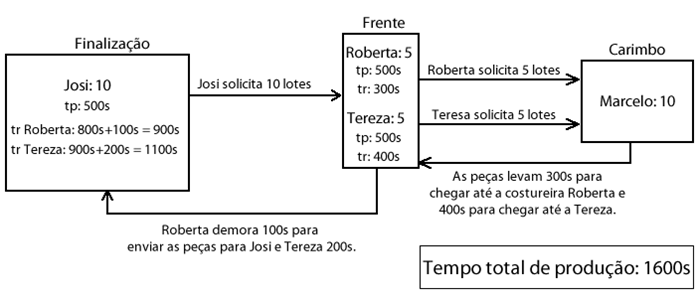
\includegraphics[scale=1.2]{./imagens/distribuicao_tempo.png}}
	\caption[Distribuição demonstrando o tempo.]
	{Distribuição demonstrando o tempo.
		\textbf{Fonte:} Desenvolvido pelos autores.}
	\label{fig:ex_tempo_producao}
\end{figure}

\par A recursividade para quando se chega na atividade Carimbo, então os valores começam a ser retornados.  
No fim, pravalece sempre o maior valor do tempo de recebimento dos lotes das atividades predecessoras e 
então tal valor é somado ao tempo de produção da finalização o que, no exemplo da Figura 17, resultou e 1600 segundos,
este valor então é colocado no atributo \texttt{tempoTotal} do indivíduo.

\par A função de avaliação é chamada dentro do método \texttt{classify}, dentro da classe \texttt{GACont\-roller}, tal método, 
por sua vez, é chamado dentro do método \texttt{execute()} após a criação da população inicial.

\subsection{Classificação dos indivíduos}
\par Uma vez definidos os valores de tempo total de produção e custo do indivíduo, o próximo passo a ser realizado, dentro da
ordem de execução do algoritmo genético, é a classificação dos indivíduos. Tal classificação também é realizada no método 
\texttt{classify} da classe \texttt{GAController}, conforme mostra o Código~\ref{list:codigo_metodo_classify}.


\begin{lstlisting} [style=custom_Java,caption={[Método \texttt{classify()}]{Método \texttt{classify()}. \textbf{Fonte:} Elaborado pelos autores.}}, label=list:codigo_metodo_classify] 
public void classify(List<Individual> population){
	List<Individual> populationAux = new ArrayList<Individual>();
	List<Individual> populationGood = new ArrayList<Individual>();
	
	for(Individual individual : population){
		individual.calculateValue();
	}
	Collections.sort(population);
		
		
	for(Individual individual : population){
			
		ProcessoIndividual pi = (ProcessoIndividual) individual;
		if(individual.getValue() <= pi.getPrazo().longValue()){
			individual.setTipoDeClassificacao(
				Constants.CLASSIFICACAO_POR_CUSTO);
				
			populationGood.add(individual);
		}
	}
	Collections.sort(populationGood);
				
	for(Individual individual : populationGood){
		individual.setTipoDeClassificacao(
			Constants.CLASSIFICACAO_POR_TEMPO);
	}
					
	//Remove todos os objetos com tempo < prazo da populacao
	population.removeAll(populationGood);
				
	//Adiciona-os na populacao auxiliar
	populationAux.addAll(populationGood);
					
	//adiciona os demais individuos da populacao
	populationAux.addAll(population);
				
	//Redefine a populacaoo
	population.clear();
	population.addAll(populationAux);
					
}
						
\end{lstlisting}

\par Após chamar a função de avaliação para todos os indivíduos, através do método \texttt{calcul\-ateValue()}, o método
de ordenação \texttt{Collections.sort()} é chamado passando a lista de indivíduos (população). Para que se possa utilizar este método
de ordenação, a classe, que representa o tipo da lista, deve implementar a interface
\texttt{Comparable} e, ao implementá-la, obrigatoriamente o método \texttt{compareTo()} deve ser implementado. Este método
define qual será o critério de comparação durante a ordenação da lista. No caso do método abstrato \texttt{compareTo} da classe \texttt{Individual}, implementado na classe \texttt{ProcessoIndividual}, foi definido uma \textit{flag} de forma a
definir se os indivíduos devem ser ordenados pelo tempo total ou pelo custo, conforme mostra o Código~\ref{list:codigo_metodo_compareTo}.

\begin{lstlisting} [style=custom_Java,caption={[Método \texttt{compareTo()}]{Método \texttt{compareTo()}. \textbf{Fonte:} Elaborado pelos autores.}}, label=list:codigo_metodo_compareTo] 

	@Override
	public int compareTo(Individual o) {
		if(tipoDeClassificacao == Constants.CLASSIFICACAO_POR_CUSTO){
			return Float.compare(getCusto(), o.getCusto());
		}else{
			return Float.compare(getTempo(), o.getTempo());
		}
	}

\end{lstlisting}

\par O atributo \texttt{tipoDeClassificacao} é iniciado com zero, ou seja, o padrão é que a classificação seja realizada levando 
em consideração o tempo total de produção de cada indivíduo. Desta forma, no Código~\ref{list:codigo_metodo_classify}, na linha
9, a ordenação da população será com base no tempo de produção. A questão é que, de acordo com o escopo definido, o objetivo do 
algoritmo seria encontrar um baixo tempo de produção associado a um custo minimizado, de forma que a melhor solução fosse aquela
que permitisse a produção das calças no menor custo com um tempo menor ou igual ao prazo, este prazo foi passado pelo usuário e
atribuído ao indivíduo no construtor da classe \texttt{ProcessoIndivíduo}, conforme já explicado na seção anterior. 

\par Desta forma, de acordo com o Código~\ref{list:codigo_metodo_classify}, após a ordenação da população pelo tempo de produção, 
é feita uma verificação para buscar todos os indivíduos que possuem tempo de produção menor ou igual ao prazo e, os indivíduos que antedem este requisito, recebem o valor 1 no atributo \texttt{tipoDeClassificacao} (ordenação por custo), alem disto são adicionados a uma outra lista denominada \texttt{populationGood}, que também será ordenada, só que agora o critério de ordenação do método \texttt{compareTo()} passou ser o custo. Após esta ordenação o atributo \texttt{tipoDeClassificacao} é zerado para evitar possíveis inconsistência em futuras ordenações e, com ajuda de listas auxiliares, os objetos da lista \texttt{populationGood} são transferidos para as primeiras posições da população e os demais indivíduos acrescentados ao final.

\par Desta forma, os melhores indivíduos (primeiros colococados), irão ter sempre menor custo, procurando manter o tempo dentro do prazo, porém caso nenhum dos indivíduos tenham o tempo total menor ou igual ao prazo, então o melhor tempo é retornado e a ordenação por custo é ignorada.

\subsection{Indivíduos estrangeiros e elitismo} \label{ind_estrangeiros_subsection}

\par Após a classificação dos indivíduos, o próximo passo, a ser realizado pelo método \texttt{execute()}, é verificar
se o melhor indivíduo (primeiro da lista) da população atual é melhor que o da população anterior, caso positivo ou
caso a população atual seja a população inicial a variável \texttt{lastBest} recebe este melhor indivíduo e então é 
realizada uma verificação para checar se o número de gerações (atributo \texttt{getGenerationQuantity}) foi atingido, 
caso positivo a execução é interrompida e o indivíduo armazenado na variável \texttt{lastBest} é retornado, ao contrário, 
a execução irá continuar de forma a iniciar a criação de uma nova população conforme mostra o Código~\ref{list:código_metodo_execute}.


\begin{lstlisting} [style=custom_Java,caption={[Método \texttt{execute()}]{Método \texttt{execute()}. \textbf{Fonte:} Elaborado pelos autores.}}, label=list:código_metodo_execute] 
	public Individual execute(){
		model.createInitialPopulation();
		Individual lastBest = null;
		
		for(int i = 0; ; i++){
			ArrayList<Individual> population = model.getPopulation();
			ArrayList<Individual> newGeneration = 
				new ArrayList<Individual>();
			
			classify(population);
			if(lastBest == null || lastBest != population.get(0)){
				lastBest = population.get(0);
			}
			
			//verifica o final da execucao
			if(i == model.getGenerationQuantity()){
				break;
			}
			
			//A partir deste ponto e iniciado a criacao de 
			//uma nova populacao
			
			//elitismo
			if(model.isElitism()){
				doElistim(newGeneration);
			}
			
			int foreignQuantity = Math.round(
				model.getPopulationSize() * model.getForeignIndividualRate());
			
			foreignQuantity = foreignQuantity % 2 == 0 ? 
				foreignQuantity : foreignQuantity +1;
			
			for(int j = 0;j < foreignQuantity;j++ ){
				newGeneration.add(model.createIndividual());
			}
			
			while(newGeneration.size() < model.getPopulationSize()){
				//selecao
				Individual individual1 = doSelection();
				Individual individual2;
				
				do{
					individual2 = doSelection();
				}while(individual1 == individual2);
				
				//cruzamento
				IndividualPair pair = doCrossing(individual1, individual2);
				
				//mutacao
				doMutation(pair.getIndividual1());
				doMutation(pair.getIndividual2());
				
				newGeneration.add(pair.getIndividual1());
				newGeneration.add(pair.getIndividual2());
			}
			
			model.setPopulation(newGeneration);
		}
		return lastBest;
	}

\end{lstlisting}

\par O processo de criação de uma nova população inicia-se com o processo de elitismo. Tal processo, conforme já explicado
anteriormente, consiste em adicionar à nova população os dois melhores indivíduos da população anterior. O próximo
passo a ser executado é referente a adição de indivíduos à nova população, seguindo um conceito, existente no \textit{framework} explicado 
na seção~\ref{framework_section}, denominado indivíduos estrangeiros. Este conceito considera o fato de que, na natureza, durante o processo de geração de uma nova população, indivíduos estrangeiros podem começar a fazer parte de tal população. 

\par No algoritmo genético, tais indivíduos simplesmente são introduzidos à nova população de acordo com uma taxa definida no 
atributo \texttt{foreignIndividualRate} da classe \texttt{GAModel} do \textit{framework}, conforme já explicado anteriormente. Conforme 
demonstrado na linha 36 do Código~\ref{list:código_metodo_execute}, os indivíduos estrangeiros são criados utilizando o método \texttt{createIndividual()} da classe \texttt{GAModel} que foi implementado na classe \texttt{ProcessoModel}, 
tal método utiliza o mesmo construtor utilizado para criação de indivíduos da população inicial portanto segue a mesma lógica utilizada, a diferença é que, ao criar tais indivíduos, o \textit{looping} é executado de acordo com a taxa definida, o que irá resultar na criação de um número bem menor de indivíduos, comparado a quantidade de indivíduos criados durante a população inicial.

\subsection{Seleção de indivíduos e cruzamento/reprodução}  \label{selecao_cruzamento_section}

\par Após o processo de elitismo e a criação dos indivíduos estrangeiros, o restante da nova população é criado através do processo
de cruzamento, conforme as instruções a partir da linha 39 do Código~\ref{list:código_metodo_execute}. O cruzamento começa com a 
seleção dos indivíduos que devem participar deste processo, esta seleção é realizada por meio do método \texttt{doSelection()} 
mostrado no Código~\ref{list:metodoDoSelection}.

\begin{lstlisting} [style=custom_Java,caption={[Método \texttt{doSelection()}]{Método \texttt{doSelection()}. \textbf{Fonte:} Elaborado pelos autores.}}, label=list:metodoDoSelection] 

private Individual doSelection() {
	switch (model.getSelectionType()) {
		case CLASSIFICATION : return doSelectionByClassification();
		case ROULETTE: return doSelectionByRoulette();
	}
	return null;
}

\end{lstlisting}

\par O método verifica o atributo de configuração \texttt{selectionType} e, neste caso, o valor de tal atributo é 
\texttt{CLASSIFICATION}, conforme mostrado na configuração do algoritmo genético na classe \texttt{GeneticAlgorithmManagement}, 
explanada anteriormente, portanto o método chamado é o \texttt{doSelectionByClassification()}, conforme mostra o Código~\ref{list:metodo_doSelectionByClassification}.

\begin{lstlisting} [style=custom_Java,caption={[Método \texttt{doSelectionByClassification()}]{Método \texttt{doSelectionByClassification()}. \textbf{Fonte:} Elaborado pelos autores.}}, label=list:metodo_doSelectionByClassification] 
	private Individual doSelectionByClassification() {
		int maxValue = 0;
		
		for(int i = 0; i< model.getPopulationSize(); i++){
			maxValue += (i + 1);
		}
		
		double index = Math.random() * maxValue;
		int cursor = 0;
		
		for(int i = 0; i < model.getPopulationSize(); i++){
			cursor += model.getPopulationSize() - 1;
			
			if(index <= cursor){
				return model.getPopulation().get(i);
			}
		}
		
		return null;
	}


\end{lstlisting}

\par Tal método é responsável pela seleção de um indivíduo para realização do cruzamento. Primeiramente
é realizado a soma dos índices da lista de indivíduos (\texttt{population}) realizando um \texttt{FOR} de 0 até
\texttt{populationSize}, parâmetro que armazena o tamanho da população, assim se o tamanho da população for
7, a soma seria 1+2+3+4+5+6+7, o que daria um total de 28. Feito esta soma, é sorteado então um número 
entre zero até a soma dos valores e então é realizado um novo \texttt{FOR} de 0 até \texttt{populationSize},
dentro deste é feita uma verificação, se o número sorteado for menor ou igual 
a ao \texttt{populationSize} (\texttt{cursor}), que neste caso é 7, então o indivíduo da posição \texttt{i} (zero) é escolhido, 
caso não seja, a variável cursor é incrementada como o valor do tamanho da população, que neste caso resultaria 
em 14 e assim a verificação é feita novamente até que o número sorteado seja menor ou igual ao cursor e, quando assim
o for, o indivíduo da posição \texttt{i} é retornado. A Figura~\ref{fig:ex_selecao} ilustra este processo.

\begin{figure}[h!]
	\centerline{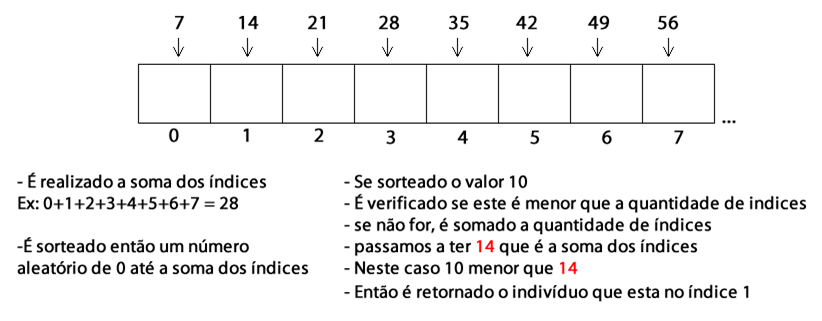
\includegraphics[scale=0.7]{./imagens/selecao.png}}
	\caption[Representação do processo de seleção dos indivíduos.]
	{Representação do processo de seleção dos indivíduos.
		\textbf{Fonte:} Desenvolvido pelos autores.}
	\label{fig:ex_selecao}
\end{figure}

\par Ao finalizar este processo um indivíduo terá sido escolhido, assim, de acordo com a linha 45 do Código~\ref{list:código_metodo_execute},
um segundo	 indivíduo deve ser selecionado, porém a instrução está dentro de um \texttt{do while} pois o processo deve ser repetido até que 
o novo indivíduo selecionado seja diferente do anterior evitando assim que dois indivíduos iguais façam parte do cruzamento.

\par O cruzamento é realizado a nível de cromossomos, de forma que, os indivíduos filhos recebem 
a mesclagem dos cromossomos de seus pais. No cruzamento desenvolvido para esta solução, foi 
necessário realizar um agrupamento dos cromossomos e então criar novos indivíduos através da
mesclagem destes grupos. Isto foi necessário pois, o total de lotes,
distribuídos entre os cromossomos de cada atividade, não pode ser diferente do número total de lotes definido, assim o 
cruzamento então ocorre de forma que os indivíduos filhos recebem a mesclagem de grupos de 
cromossomos de seus pais referente a cada atividade e assim a cada cruzamento é criado
dois novos indivíduos que irão fazer parte da nova população. A Figura~\ref{fig:ex_cruzamento} ilustra este processo.

\newpage

\begin{figure}[h!]
	\centerline{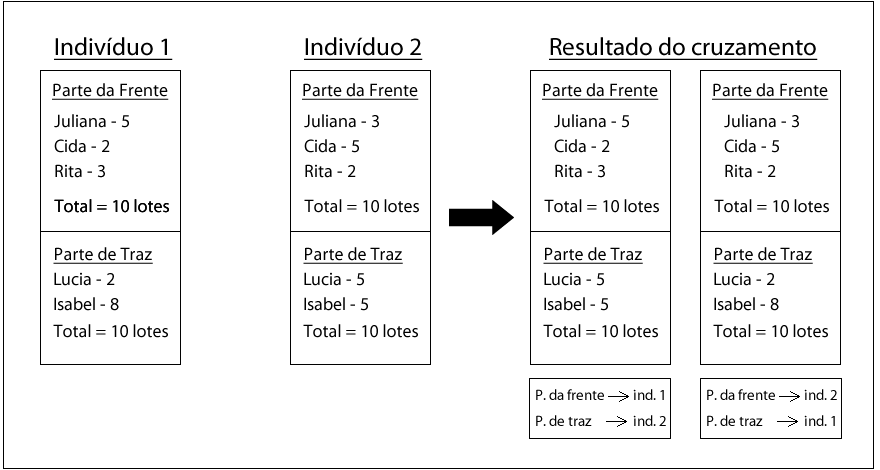
\includegraphics[scale=0.4]{./imagens/ex_cruzamento.png}}
	\caption[Cruzamento dos indivíduos.]
	{Cruzamento dos indivíduos.
		\textbf{Fonte:} Desenvolvido pelos autores.}
	\label{fig:ex_cruzamento}
\end{figure}


\par A partir da linha 49 do código Código~\ref{list:código_metodo_execute}, dois indivíduos já foram selecionados e então o 
método \texttt{doCrossing()} é chamado para realizar o cruzamento. Tal método também verifica o tipo de cruzamento definido
chamando o método correspondente conforme mostra o Código~\ref{list:metodoDoCrossing}. 



\begin{lstlisting} [style=custom_Java,caption={[Método \texttt{doCrossing()}]{Método \texttt{doCrossing()}. \textbf{Fonte:} Elaborado pelos autores.}}, label=list:metodoDoCrossing] 
	private IndividualPair doCrossing(Individual individual1, 
		Individual individual2){
		
		switch (model.getCrossType()) {
			case ARITMETIC: break;
			
			case BINARY: 
				return doBinaryCrossing(individual1,individual2);
			case PERMUTATION: 
				return doPermutationCrossing(individual1, individual2);
		
			case UNIFORM:break;
		}
		return null;
	}

\end{lstlisting}


\par Neste caso, o método escolhido para o cruzamento foi o de permutação, desta forma o método \texttt{doPermutationCrossing()} é chamado.
Tal método faz parte do \textit{framework} de desenvolvimento, porém foi modificado para se adaptar ao problema a ser resolvido pela 
aplicação conforme demonstrado no Código~\ref{list:metodoPermutationCrossing}.


\begin{lstlisting} [style=custom_Java,caption={[Método \texttt{doPermutationCrossing()}]{Método \texttt{doPermutationCrossing()}. \textbf{Fonte:} Elaborado pelos autores.}}, label=list:metodoPermutationCrossing] 
		private IndividualPair doPermutationCrossing(
			Individual individual1, Individual individual2){
			
			ArrayList<Chromosome> chromosomes1 = 
				new ArrayList<Chromosome>();
				
			ArrayList<Chromosome> chromosomes2 = 
				new ArrayList<Chromosome>();
				
			Integer lastAtividade = null;
			float chooseIndividual = 0;
			int i = 0;
			
			for(Chromosome chromosome : individual1.getChromosomes()){
				ProcessoChromosome processoChromosome = 
					(ProcessoChromosome) chromosome;
				
				if(lastAtividade == null || 
					!lastAtividade.equals(processoChromosome.getAtividade())){
					
					chooseIndividual = Math.round((float) Math.random() * 1);
					lastAtividade = processoChromosome.getAtividade();
				}
				
				if(chooseIndividual == 1){
					chromosomes1.add(individual1.getChromosomes().
						get(i).clone());
						
					chromosomes2.add(individual2.getChromosomes().
						get(i).clone());
				}else{
					chromosomes1.add(individual2.getChromosomes().
						get(i).clone());
						
					chromosomes2.add(individual1.getChromosomes().
						get(i).clone());
				}
				i++;
			}
			
			Individual newIndividual1 = 
				model.createIndividual(chromosomes1);
				
			Individual newIndividual2 = 
				model.createIndividual(chromosomes2);
			
			return new IndividualPair(newIndividual1,newIndividual2);
		}
	

\end{lstlisting}

\par Conforme visto na Figura~\ref{fig:ex_cruzamento}, os cromossomos estão ordenados na lista de acordo com suas respectivas atividades, considerando isto, foi feita uma lógica para agrupar estes cromossomos por atividade e criar novos indivíduos através da mesclagem dos grupos criados de forma a sortear de qual indivíduo do cruzamento cada grupo deve ser pego ao criar um novo indivíduo. 

\par Assim, de acordo com o Código~\ref{list:metodoPermutationCrossing}, primeiramente é feita uma iteração sobre a lista de cromossomos do indivíduo 1, dentro de tal iteração, é realizada uma verificação para checar se um cromossomo é o primeiro da primeira atividade (\texttt{lastAtividade == null}) ou se é o primeiro de um determinada atividade de acordo com a ordem delas, caso uma destas condições for verdadeira, um valor binário é sorteado, se tal valor for um, o primeiro novo indivíduo que será criado terá os cromossomos da atividade em questão, pegos do indivíduo 1 do cruzamento e o segundo novo indivíduo receberá os cromossomos, referentes a tal atividade, do indivíduo 2, caso o valor sorteado seja zero, o processo acontece de forma inversa. 

\par Assim a iteração continua até a lista de cromossomos dos novos indivíduos possuir todos os grupos de cromossomos referentes a todas as atividades e então, ao fim da iteração, dois novos indivíduos serão criados através do método \texttt{createIndividual()}.

\par Quando se cria indivíduos a partir deste ponto, a classe \texttt{ProcessoModel} utiliza um outro construtor para criar o indivíduo, conforme mostra o Código~\ref{list:metodoCreateIndividualCromossomos}.


\begin{lstlisting} [style=custom_Java,caption={[Método \texttt{createIndividual()} utilzando cromossomos]{Método \texttt{createIndividual()} utilizando cromossomos. \textbf{Fonte:} Elaborado pelos autores.}}, label=list:metodoCreateIndividualCromossomos] 
	@Override
	public Individual createIndividual(
		ArrayList<Chromosome> chromosomes) {
		
		return new ProcessoIndividual(atividadeFinal,
			 prazoEmSegundos, chromosomes,this.numeroLote,
				 this.pecasPorLote);
	}

\end{lstlisting}

\par Neste caso são passados quase todos os parâmetros enviados durante a criação
da população inicial, a diferença é que o indivíduo será criado a partir 
dos cromossomos conforme mostra o Código~\ref{list:construtorDeIndividuosComCromossomos}.

\begin{lstlisting} [style=custom_Java,caption={[Construtor de \texttt{ProcessoIndividual} utilizando cromossomos]{Construtor de \texttt{ProcessoIndividual} utilizando cromossomos. \textbf{Fonte:} Elaborado pelos autores.}}, label=list:construtorDeIndividuosComCromossomos] 
public ProcessoIndividual(Atividade atividadeInicial, 
						  BigDecimal prazoEmSegundos, 
						  ArrayList<Chromosome> chromosomes, 
						  int numeroLote, int pecasPorLote) {

	super(chromosomes);
	this.atividadeFinal = atividadeInicial;
	this.numeroLote = numeroLote;
	this.pecasPorLote = pecasPorLote;
	this.prazo = prazoEmSegundos;
}

\end{lstlisting}
\par Os cromossomos recebidos são inseridos na lista de cromossomos declarada na classe mãe (\texttt{Individual}), e os 
outros parâmetros são atribuídos aos seus respectivos atributos. No final do método \texttt{doPermutaionCrossing}, como no 
Java não é possível retornar dois valores, é criado um objeto da classe \texttt{IndividualPair}, passando os dois novos indivíduos, 
e então este objeto é retornado. Esta classe só possui dois atributos do tipo \texttt{Individual} e só é utilizada para retornar os dois 
novos indivíduos criados.

\subsection{Mutação} \label{mutacao_subsection}
\par O processo de mutação, conforme já explicado anteriormente, consiste em realizar uma pequena modificação entre os cromossomos
de um indivíduo. Esta modificação pode ser boa, melhorando o resultado do indivíduo ou ruim. No algoritmo genético desenvolvido, 
a mutação foi realizada trocando o número de lotes recebidos entre duas costureiras escolhidas aleatoriamente dentro cada grupo de cromossomos (atividades) do indivíduo, conforme mostra a Figura~\ref{fig:ex_mutacao}.

\begin{figure}[h!]
	\centerline{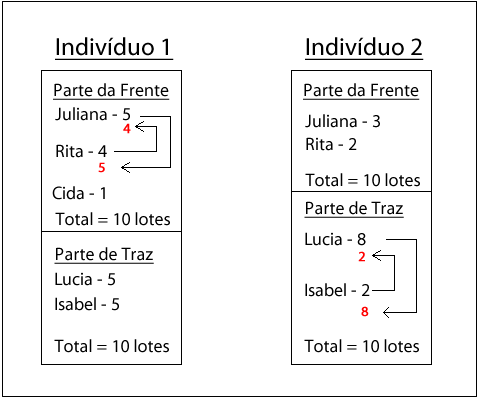
\includegraphics[scale=0.7]{./imagens/mutacao_cromossomo.png}}
	\caption[Exemplo de mutação.]
	{Exemplo de mutação.
		\textbf{Fonte:} Desenvolvido pelos autores.}
	\label{fig:ex_mutacao}
\end{figure}


\par O processo de mutação inicia-se logo após cada cruzamento e é realizado
nos indivíduos criados neste processo, dentro de uma determinada taxa, definida anteriormente nos atributos de configuração do algoritmo genético na classe \texttt{GeneticAlgorithmManagement}. O método que inicia este processo é o \texttt{doMutation()}, que verifica o tipo de mutação definido, chamando o método correspondente, além disto, ele verifica se a mutação deve ser realizada, sorteando um número aleatoriamente e checando se o número sorteado é menor que a taxa de mutação definida, conforme mostra o Código~\ref{list:metodoDoMutation}. 

\begin{lstlisting} [style=custom_Java,caption={[Método \texttt{doMutation()}]{Método \texttt{doMutation()}. \textbf{Fonte:} Elaborado pelos autores.}}, label=list:metodoDoMutation] 
	public void doMutation(Individual individual){
		if(Math.random() < model.getMutationRate()){
			for(int i = 0; i < model.getMutationQuantity();i++){
				switch (model.getMutation()) {
					case BINARY: doMutationBinary(individual);break;
					case NUMERICAL: break;
					case PERMUTATION: doMutationPermutation(individual);break;
				}
			}
		}
	}

\end{lstlisting}

\par Neste caso, o método escolhido para a mutação foi o \texttt{PERMUTATION}, desta forma o método \texttt{doMutationPermutation()} é chamado.
Tal método faz parte do \texttt{framework} de desenvolvimento, porém também foi modificado para se adaptar ao problema a ser resolvido pela 
aplicação, conforme demonstrado no Código~\ref{list:metodoPermutationMutation}.


\begin{lstlisting} [style=custom_Java,caption={[Método \texttt{doMutationPermutation()}]{Método \texttt{doMutationPermutation()}. \textbf{Fonte:} Elaborado pelos autores.}}, label=list:metodoPermutationMutation] 
	public void doMutationPermutation(Individual individual) {
	
		Integer lastAtividade = null;
		ArrayList<ProcessoChromosome> chromossomesToMutate = 
			new ArrayList<ProcessoChromosome>(); 
		
		for(Chromosome chromosome : individual.getChromosomes()){
			ProcessoChromosome processoChromosome = 
				(ProcessoChromosome) chromosome;
			
			if(lastAtividade == null || 
				   !lastAtividade.equals(processoChromosome.getAtividade())){
				   
				if(!chromossomesToMutate.isEmpty() && 
					   chromossomesToMutate.size() > 1){
					
					doMutationOnChromossome(chromossomesToMutate);
				}
				chromossomesToMutate.clear();
				lastAtividade = processoChromosome.getAtividade();
			}
			chromossomesToMutate.add(processoChromosome);
		}
		//Para o ultimo grupo
		if(!chromossomesToMutate.isEmpty() && 
			   chromossomesToMutate.size() > 1){
			
			doMutationOnChromossome(chromossomesToMutate);
		}
	}

\end{lstlisting}

\par A lógica que faz a mutação, inicia-se com uma iteração na lista de cromossomos do 
indivíduo a qual a mutação será realizada, dentro desta iteração, os cromossomos de uma atividade são adicionados
à lista \texttt{chromossomesToMutate}, e assim, quando todos os cromossomos de uma atividade são adicionados nesta
lista, o método \texttt{doMutationOnCromossome}, demonstrado no Código~\ref{list:metododoMutationOnChromossome}, é
chamado para realizar a mutação, assim, após a mutação para os cromossomos de tal atividade, a lista \texttt{chromossomesToMutate} é zerada para que os cromossomos da próxima atividade sejam adicionados a esta e posteriormente sofram a mutação, logicamente, o grupo de atividades sofrerá mutação somente se possuir mais de um cromossomo.

\begin{lstlisting} [style=custom_Java,caption={[Método \texttt{doMutationOnChromossome()}]{Método \texttt{doMutationOnChromossome()}. \textbf{Fonte:} Elaborado pelos autores.}}, label=list:metododoMutationOnChromossome] 
	private void doMutationOnChromossome(
		ArrayList<ProcessoChromosome> chromossomesToMutate){
	
		int position1;
		int position2;
		int varAux;
		int varAux2;
		
		ProcessoChromosome chromosome1 = null;
		ProcessoChromosome chromosome2 = null;
		
		position1 = (int) (Math.random() * (chromossomesToMutate.size()));
		
		do{
			position2 = (int) (Math.random() * 
				(chromossomesToMutate.size()));
		}while(position1 == position2);
	
		chromosome1 = chromossomesToMutate.get(position1);
		chromosome2 = chromossomesToMutate.get(position2);
		
		varAux  = chromosome2.getQuantidade_lotes();
		varAux2 = chromosome2.getLotesToShow();
		
		chromosome2.setQuantidade_lotes(
			chromosome1.getQuantidade_lotes());
			
		chromosome2.setLotesToShow(chromosome1.getLotesToShow());
		
		chromosome1.setQuantidade_lotes(varAux);
		chromosome1.setLotesToShow(varAux2);
	}

\end{lstlisting}

\par Neste método, é selecionado quais cromossomos terão seus valores trocados entre si. O segundo cromossomo é escolhido dentro da 
estrutura de repetição \texttt{do While}, para evitar que o mesmo cromossomo escolhido na primeira vez seja selecionado e então, com auxilio de variáveis auxiliares, os atributos \texttt{quantidade\_lotes} e \texttt{lotesToShow}, tem seus valores trocados entre si. O atributo \texttt{lotesToShow} é utilizado para espelhar a quantidade de lotes do indivíduo. Este atributo é necessário pois, no processo de avaliação dos indivíduos, as costureiras (cromossomos) das primeiras atividades consomem lotes dos cromossomos das atividades predecessoras, decrementando assim o atributo \texttt{quantidade\_lotes} do cromossomo, assim o atributo \texttt{lotesToShow} é utilizado para manter o valor de lotes original dos cromossomos para mostrar no resultado da distribuição quantos lotes cada costureira recebeu.

Concluindo, após a finalização do processo de cruzamento e possível mutação dos novos indivíduos, uma nova população terá sido criada, assim esta nova população substitui a população anterior e então todo o processo de classificação, verificação do melhor indivíduo etc é reiniciado, desta forma sempre será criada uma nova população até que o número de gerações seja atingido e quando o for, o melhor indivíduo 
é retornado, conforme explicado anteriormente. 

\subsection{Interface gráfica de distribuição} \label{interface_grafica_section}

\par Para a interação do usuário com o algoritmo de distribuição e possibilidade de cadastro de fluxos de processos e 
costureiras, bem como suas respectivas habilidades, tempo e preço de produção, foi realizado uma aplicação em plataforma \textit{web}
utilizando \textit{JSF} e \textit{Primefaces}. A forma que o mecanismo de cadastro das informações foi realizado não é relevante
ser apresentado, sendo importante porém, explanar sobre o desenvolvimento da tela de distribuição das atividades, a qual é de extrema importância para entender o fluxo de execução da aplicação. No menu "Distribuir tarefas" da aplicação estão disponíveis todos os processos cadastrados e para abrir a tela de distribuição de atividades basta clicar no ícone "Abrir" da coluna opções conforme mostra a Figura~\ref{fig:tela_dis_processos}.

\begin{figure}[h!]
	\centerline{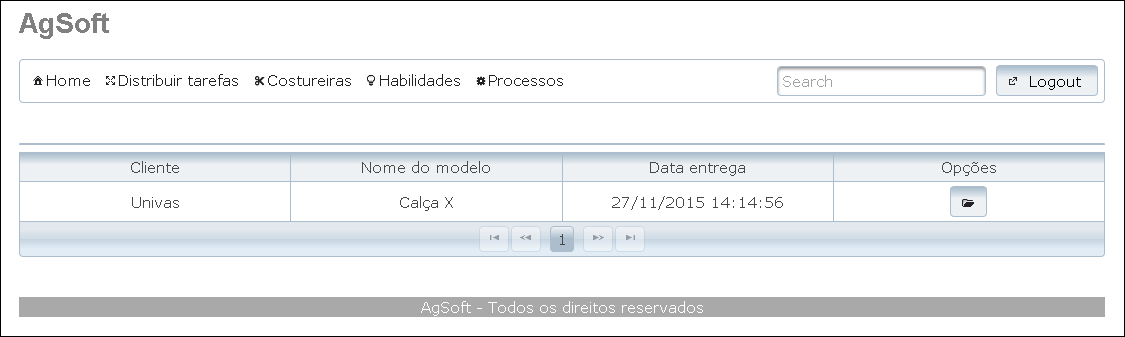
\includegraphics[scale=0.5]{./imagens/tela_distribuicao_processos.png}}
	\caption[Menu Distribuir tarefas.]
	{Menu Distribuir tarefas.
		\textbf{Fonte:} Desenvolvido pelos autores.}
	\label{fig:tela_dis_processos}
\end{figure}

\par Ao clicar no ícone "Abrir", é aberta uma tela de distribuição para aquele processo, que é responsável por captar alguns
dados importantes para a regra de negócio do algoritmo genético, além disto, é nela que as informações do melhor indivíduo (melhor
solução) são apresentadas.  Os dados informados através desta tela são o número total de peças que se deseja produzir, o número de 
peças que cada lote irá conter e a data de início da produção conforme mostra a Figura~\ref{fig:tela_dis_open}.

\newpage

\begin{figure}[h!]
	\centerline{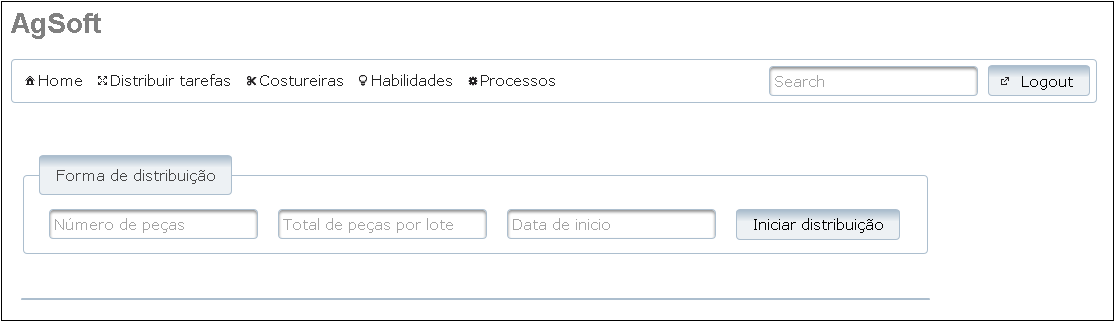
\includegraphics[scale=0.5]{./imagens/tela_distribuicao_open.png}}
	\caption[Tela de distribuição de tarefas.]
	{Tela de distribuição de tarefas.
		\textbf{Fonte:} Desenvolvido pelos autores.}
	\label{fig:tela_dis_open}
\end{figure}

\par Toda tela criada com \texttt{JSF} é desenvolvida através de documentos \texttt{XHTML}, tais documentos possuem componentes para entrada e apresentação dos dados. Estes componentes podem ser tanto do \texttt{JSF} quanto do \textit{primefaces}, o Código~\ref{list:doc_xhtml} demonstra o documento \texttt{XHTML} da tela demonstrada acima.

\begin{lstlisting} [style=custom_Java,caption={[Documento XHTML da tela de distribuição]{Documento XHTML da tela de distribuição. \textbf{Fonte:} Elaborado pelos autores.}}, label=list:doc_xhtml] 
<?xml version="1.0" encoding="UTF-8"?>
<ui:composition xmlns="http://www.w3.org/1999/xhtml"
xmlns:ui="http://java.sun.com/jsf/facelets"
xmlns:f="http://java.sun.com/jsf/core"
xmlns:h="http://java.sun.com/jsf/html"
xmlns:p="http://primefaces.org/ui">

<h:form id="formAbrirProcessoDis">
	<p:messages autoUpdate="true"></p:messages>
	
	<p:panelGrid columns="1">
	
		<div id="distribuicaoFields">
			<p:fieldset legend="Forma de distribuicao">
				<p:panelGrid columns="4">
					<p:inputText id="nPecas" required="true" 
					value="#{distribuicaoController.totalPecas}"
					requiredMessage="Por favor informe o total de pecas" 
					maxlength="19" placeholder="Numero de pecas" />
					
					<p:inputText id="totalPecaPorLote" required="true"
					value="#{distribuicaoController.totalPecasPorLote}"
					requiredMessage="Por favor informe o total 
						de pecas por lote"
						
					maxlength="19" placeholder="Total de pecas por lote"/>
					
					<p:calendar id="inicio" required="true"
								mask="true" effect="fold"
								value="#{distribuicaoController.dataInicio}"
								requiredMessage="Por favor informe uma data de inicio" 
								pattern="dd/MM/yyyy HH:mm:ss" 
									mindate="#{processosController.getCurrentDate()}"
					
								maxdate="#{distribuicaoController.getDataEntrega()}"
								placeholder="Data de inicio"/>
					
					<p:commandButton action="#{distribuicaoController.
						iniciarDistribuicao()}"
					
					value="Iniciar distribuicao" 
					update="formAbrirProcessoDis"
					ajax="true" onstart="PF('waitDialog').show();"
					onsuccess="PF('waitDialog').hide();"/>
				
				</p:panelGrid>
			</p:fieldset>
		</div>
	.
	.
	.

\end{lstlisting}

\par No \texttt{JSF}, toda página \texttt{XHTML} possui um controlador que
consiste em uma classe Java, e para definir que tal classe é uma controladora de páginas, na sua declaração é definida a anotação \texttt{@ManagedBean(name = "[nome da classe em minusculo]")}.
No caso da tela de distribuição, a classe controladora é denominada \texttt{DistribuiçãoController}, portanto possui a notação
\texttt{@ManagedBean(name = "[distribuiçãoController]")} em sua declaração. As páginas \texttt{XHTML} fazem então um \textit{bind}, ou
seja, uma conexão com a classe controladora de forma que os dados do \texttt{XHTML} são disponibilizados em tal classe e vice-versa. 
No caso da página de distribuição, as \textit{tags} \texttt{p:inputText} e \texttt{p:calendar} são responsáveis pela entrada de 
informações, tais \textit{tags} possuem um atributo \texttt{value}, neste atributo é informado em qual classe controladora e em qual 
atributo desta os dados informados pelo usuário serão atribuídos, realizando assim o \textit{bind}. Neste caso os dados informados pelo 
usuário estarão respetivamente disponíveis nos atributos \texttt{totalPecas}, \texttt{totalPecasPorLote} e \texttt{dataInicio} da
classe \texttt{DistribuiçãoController}.

\par Após entrar com os dados necessários, o usuário deve clicar no botão "Iniciar Distribuição", este botão é construído com a
\textit{tag} \texttt{p:commandButton} conforme mostra o Código~\ref{list:doc_xhtml}. Esta \textit{tag} possui o atributo \texttt{action} que 
é responsável por chamar um método da classe controladora para executar uma determinada ação, neste caso, o método chamado é o 
\texttt{iniciarDistribuicao()} responsável por iniciar a distribuição das atividades chamando o gerenciador do algoritmo genético, 
conforme mostra o Código~\ref{list:metodoiniciarDistribuicao}.

\begin{lstlisting} [style=custom_Java,caption={[Método \texttt{iniciarDistribuicao()}]{Método \texttt{iniciarDistribuicao()}. \textbf{Fonte:} Elaborado pelos autores.}}, label=list:metodoiniciarDistribuicao] 

public void iniciarDistribuicao(){
	int totalPecasInt = Integer.parseInt(totalPecas);
	int totalPecasPorLoteInt = Integer.parseInt(totalPecasPorLote);
	
	if(totalPecasInt == 0 || totalPecasPorLoteInt == 0){
		sendMessageToView(
			"Total de pecas ou total de pecas por lote e invalido!", 
				FacesMessage.SEVERITY_ERROR);
		return;
	}
	
	numeroDeLotes = totalPecasInt / totalPecasPorLoteInt;
	if((numeroDeLotes * totalPecasPorLoteInt) != totalPecasInt){
		sendMessageToView("Numero de lote nao exato: "+numeroDeLotes+" * "
			+ totalPecasPorLote+" = "+numeroDeLotes*totalPecasPorLoteInt, 
				FacesMessage.SEVERITY_ERROR);
		return;
	}
	
	if(idProcesso <= 0 || processo == null){
		sendMessageToView(
			"Processo invalido", FacesMessage.SEVERITY_ERROR);
		
		return;
	}
	
	prazEmSegundos = calcularPrazo();
	prazoAtendido = false;
	
	GeneticAlgorithmManagement gam = new GeneticAlgorithmManagement();
	melhorIndividuo = gam.iniciarDistribuicao(
		numeroDeLotes, prazEmSegundos, totalPecasPorLoteInt, idProcesso);
	
	//This is just to manage information messages in the view
	if(melhorIndividuo.getValue() <= prazEmSegundos.longValue()){
		prazoAtendido = true;
	}
	
	if(melhorIndividuo != null){
		rootFluxograma = construirArvore(melhorIndividuo.getNode(), null);
		allNodes = new ArrayList<Node>();
		rootTable  = 
			new DefaultTreeNode(
				new TabDetailBean("-", "-", "-","-","-","-","-"));
	
		construirTableDetail(melhorIndividuo);
		mostrarResult = true;
	}
}

\end{lstlisting}

\ Os dados que o algoritmo genético espera receber são número de lotes a serem distribuídos, o número de 
peças por lote e o prazo de entrega. Portanto uma das funções do método \texttt{iniciarDistribuicao()} é
calcular a quantidade de lotes a serem produzidos e o prazo de entrega das peças, além disto, o método 
realiza algumas validações, de forma a somente enviar informações consistentes para o algoritmo genético. 
O cálculo de número de lotes é realizado então dividindo o número de peças informado pelo usuário pelo 
número de peças por lote, o resultado é armazenado na variável \texttt{numeroDeLotes}.

\par Para calcular o prazo de entrega da produção é chamado o método \texttt{calcularPrazo()} demonstrado no 
Código~\ref{list:metodoCalcularPrazo}.

\begin{lstlisting} [style=custom_Java,caption={[Método \texttt{calcularPrazo()}]{Método \texttt{calcularPrazo()}. \textbf{Fonte:} Elaborado pelos autores.}}, label=list:metodoCalcularPrazo] 

public BigDecimal calcularPrazo(){
	DateTime dataInical = new DateTime(dataInicio);
	DateTime dataFinal  = new DateTime(processo.getDataEntrega());
	return  new BigDecimal(Seconds.secondsBetween(dataInical, dataFinal).getSeconds());
}

\end{lstlisting}

\par É importante observar que o prazo é calculado em segundos, devido ao fato que o tempo de produção por peça e o tempo 
de transporte entre as costureiras são definidos em segundos. O método \texttt{calcularPrazo()} simplesmente retorna o tempo 
em segundos entre a data de início, informada pelo usuário e disponível no atributo \texttt{dataInicio} e o prazo de entrega, 
disponível no atributo \texttt{dataEntrega} do processo que foi informada no cadastro do mesmo. É importante ressaltar que
o objeto \texttt{processo} utilizado neste método foi criado no momento em que o usuário abriu o processo, neste caso, foi enviado
o \texttt{ID} do tal processo via \texttt{URL} e o controlador buscou, no banco de dados as informações do mesmo através deste \texttt{ID} criando assim tal objeto.

\par Após o calculo do número de lotes e do prazo, é instanciado um objeto da classe 
\texttt{GeneticAlgorithmManagement}, conforme explicado anteriormente, e então o método 
\texttt{inici\-arDistribuicao()} é chamado. Tal método, conforme já visto nas seções anteriores,
faz o gerenciamento da execução do algoritmo genético e retorna o melhor indivíduo encontrado, tal indivíduo é armazenado no 
atributo \texttt{melhorIndividuo} da classe \texttt{distribuiçãoController} e então os métodos \texttt{construirArvore()} e
\texttt{construirTableDetail()} são chamados para realizar a apresentação dos dados do indivíduo na tela após a distribuição, tais métodos
simplesmente apresentam ao usuário as atividades e suas respectivas costureiras juntamente com o número de lote que cada uma recebeu, além disto, também é apresentado o tempo e o custo total, além de uma tabela de detalhes da distribuição.
A Figura~\ref{fig:tela_dis_result} mostra a tela com o resultado da execução do algoritmo.

\begin{figure}[h!]
	\centerline{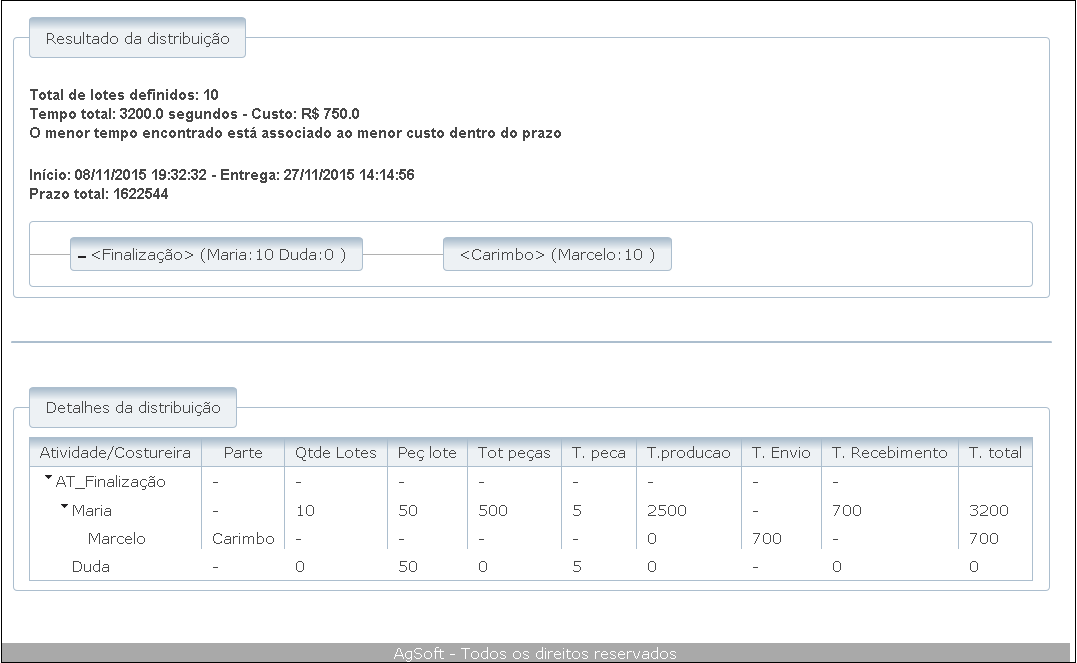
\includegraphics[scale=0.4]{./imagens/resultado_distribuicao.png}}
	\caption[Tela de resultado de distribuição de tarefas.]
	{Tela de resultado de distribuição de tarefas.
		\textbf{Fonte:} Desenvolvido pelos autores.}
	\label{fig:tela_dis_result}
\end{figure}

\par Os resultados serão vistos com mais detalhes nos casos de testes apresentados na discussão de resultados.

% \label{cap:quadroMetodologico}
% 
% \par Conteúdo do quadro metodológico. Perceba a forma que se coloca uma palavra entre aspas: o \LaTeX~oferece muita ``facilitade de formatação''.
% 
% Exemplo de código Java:
% 
% \begin{lstlisting} [style=custom_Java,caption={[Métodos da classe \texttt{FilmeBean}]{Métodos da classe \texttt{FilmeBean}. \textbf{Fonte:} Elaborado pelos autores.}}, label=fig:metodosclassebean] 	
% 	public FilmeBean(){  
%        //...
%    	}	
%    	
% 	public void saveMovie(){
% 		setListActorSelected();		
% 		if(this.movieDAO.saveMovieGraph(this.movieTo)){
% 			FacesContext.getCurrentInstance().addMessage(null, 
% 			   new FacesMessage("Filme cadastrado com sucesso!")); 
% 		}else{
% 			//...
% 		}		
% 		this.limpaCampos();
% 	}
% \end{lstlisting}
% 
% \par Agora será mostrado o exemplo do uso de fluxo de eventos apresentado no Quadro~\ref{quad:fluxo_evento_cadastro_filme}.
% 
% \begin{quadro}[h!]
%   \begin{fluxoDeEventos}
  \addTitle{Cadastrar filme}
  \addrow{Ator principal}{Administrador}
  %\addrow{Ator secundário}{Sistema de cartão}
  \addrow{Pré-requisitos}{Estar logado no sistema}

  \startBasicFlow{Ator} {Sistema}
  \addItemOne{Seleciona menu cadastro}
  \addItemOne{Clica na opção cadastrar filme}
  \addItemTwo{Abre interface de cadastro de filme}
  \addItemOne{Preenche formulário}
  \addItemOne{Clica no botão salvar}
  \addItemTwo{Salva e informa sucesso no cadastro}

  \startAlternativeFlow{Fluxo alternativo 1}
  \addItemOne{No item 5, formulário não preenchido}
  \addItemTwo{Exibe mensagem de necessidade de preenchimento de formulário}

  \startAlternativeFlow{Fluxo alternativo 2}
  \addItemOne{No item 6, inserido filme já cadastrado}
  \addItemTwo{Informa mensagem de filme já cadastrado}
\end{fluxoDeEventos}

%   \caption[Fluxo de eventos para cadastro de filme]
%            {Fluxo de eventos para cadastro de filme. \textbf{Fonte:} Elaborado pelos autores}
%   \label{quad:fluxo_evento_cadastro_filme}
% \end{quadro}
% 
% \par Outro exemplo é ilustrado na Figura~\ref{fig:bluesky}. Neste caso um código XML foi embutido dentro de um ambiente de figura, para que este código seja incluído no índice de figuras adequadamente.
%  
% \begin{figure}[ht!]
%   \begin{lstlisting} [style=custom_XML]
% 	...
% 	<context-param>
% 		<param-name>primefaces.THEME<\param-name>
% 		<param-value>bluesky<\param-value>
% 	<\context-param>
% 	...
%   \end{lstlisting}
%   \caption[Incluindo o tema \textit{BlueSky} ao contexto do projeto]
%           {Incluíndo o tema \textit{BlueSky} ao contexto do projeto. \textbf{Fonte:} Elaborado pelos autores.}
%   \label{fig:bluesky}
% \end{figure}

%\input{editaveis/design}
%\chapter{Discussão de resultados}

\par Neste capítulo serão apresentados e discutidos os resultados obtidos pela pesquisa e implementação 
do sistema de otimização do processo de fabricação de calças. Tal discussão será realizada em forma de
casos de teste, buscando demonstrar o comportamento do algoritmo genético de diferentes formas.

\par Desde o princípio, quando começou-se a discutir sobre o tema do 
trabalho de conclusão de curso, teve-se a ideia de desenvolver algo relacionado
à inteligência artificial, por ser um assunto de bastante relevância na área de desenvolvimento de software. 
Dentro deste campo então, realizando algumas buscas na internet, foi encontrado
o assunto de algoritmos genéticos.
Coincidentemente foi lecionada no primeiro semestre deste ano a disciplina
sistemas especialistas, a qual o assunto foi abordado o que facilitou bastante o aprendizado.

\par Assim, como sugestão do professor orientador, foi decidido então
desenvolver uma aplicação para otimizar um processo de distribuição de atividades entre
costureiras para um microempresário da cidade de Cachoeira de Minas - MG, do ramo de costura e constatamos 
que um sistema Web seria mais cômodo de ser utilizado por não precisar de
nenhuma instalação por parte do usuário e este poder acessar o programa de
qualquer lugar desde que estivesse conectado à internet.

\par Neste sentido, foram adotadas como tecnologias para o desenvolvimento em
plataforma Web os \textit{frameworks} JSF e Primefaces. Além disso foi utilizado
um \textit{plug-in} denominado \texttt{JBoss Tools} o qual foi de grande utilidade para gerar as classes 
modelos a partir do banco de dados.

\par Inicialmente foi tomado como base o caso do microempresário citado acima,
todavia logo após iniciarmos o trabalho, o mesmo fez uma reestruturação de processos em sua empresa. 
Desta forma, sua maneira de trabalhar deixou de ser um cenário o qual algoritmos genéticos
pudessem ser aplicados, desta forma, fechou-se um escopo para que o trabalho
pudesse continuar, conforme descrito na seção 3.3.2 do quadro metodológico. Com
o escopo definido, o foco passou a ser na definição da estrutura dos elementos do algoritmo genético.



\par Assim, seguindo os passos descritos no quadro metodológico, foi obtido como resultado a aplicação
capaz de distribuir atividades de forma a se obter o menor custo e o menor tempo de produção, 
alcançando assim os objetivos específicos. Com a aplicação finalizada, foram realizados então casos de 
testes a fim de colocar em prova a eficiência da ferramenta para se buscar melhores soluções nas distribuição 
de tarefas, conforme mostra as seções seguintes.


\section{Teste considerando somente o tempo de produção}

\par Este teste demonstra a distribuição de lotes levando em consideração o
tempo de cada costureira para fabricação das peças. Neste teste será definido o
preço por peça igual para as costureiras alterando somente o tempo por peça de
cada uma. Para este teste foi cadastrado um processo de produção informando o
cliente, o modelo da calça e a data e hora da entrega conforme mostra a Figura~\ref{fig:cad_processo1}.

\begin{figure}[h!]
	\centerline{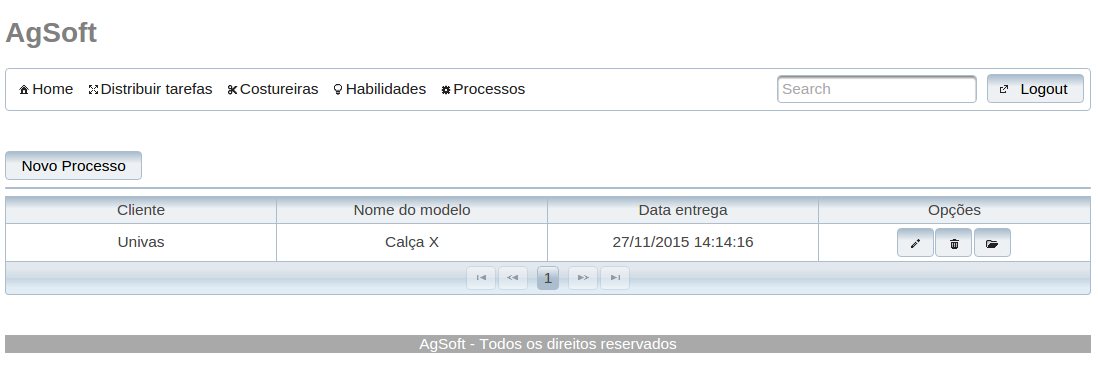
\includegraphics[scale=0.4]{./imagens/teste_processo.png}}
	\caption[Criação de um processo.]
	{Criação de um processo. \textbf{Fonte:} Desenvolvido pelos autores.}
	\label{fig:cad_processo1}
\end{figure}

\par Todo processo ao ser criado, por padrão já contém as atividades principais
 Carimbo e Finalização conforme mostra a Figura~\ref{fig:processo_cadastrado}.

\begin{figure}[h!]
	\centerline{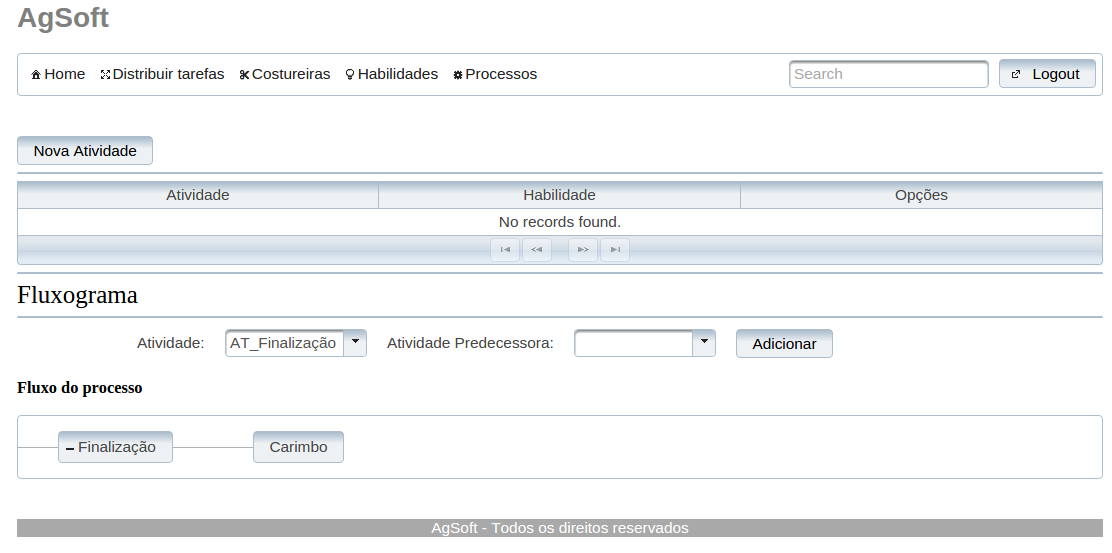
\includegraphics[scale=0.3]{./imagens/tela_processo_teste1.png}}
	\caption[Detalhes do processo cadastrado.]
	{Detalhes do processo cadastrado. \textbf{Fonte:} Desenvolvido pelos autores.}
	\label{fig:processo_cadastrado}
\end{figure}

\par Após a criação do processo foram definidas quais costureiras possuem a
habilidade para realizar as atividades que compõe o processo, sendo definidas para 
realizar a atividade finalização, as costureiras Maria e Duda, ambas cobram o 
mesmo valor por peça porém o tempo gasto para fabricar uma peça é diferente 
conforme mostra a Figura~\ref{fig:costureira_habilidade}. Vale ressaltar que
a atividade carimbo é realizada somente pelo proprietário da fábrica pois é a
atividade onde serão distribuídas as peças para serem produzidas. 


\begin{figure}[h!]
	\centerline{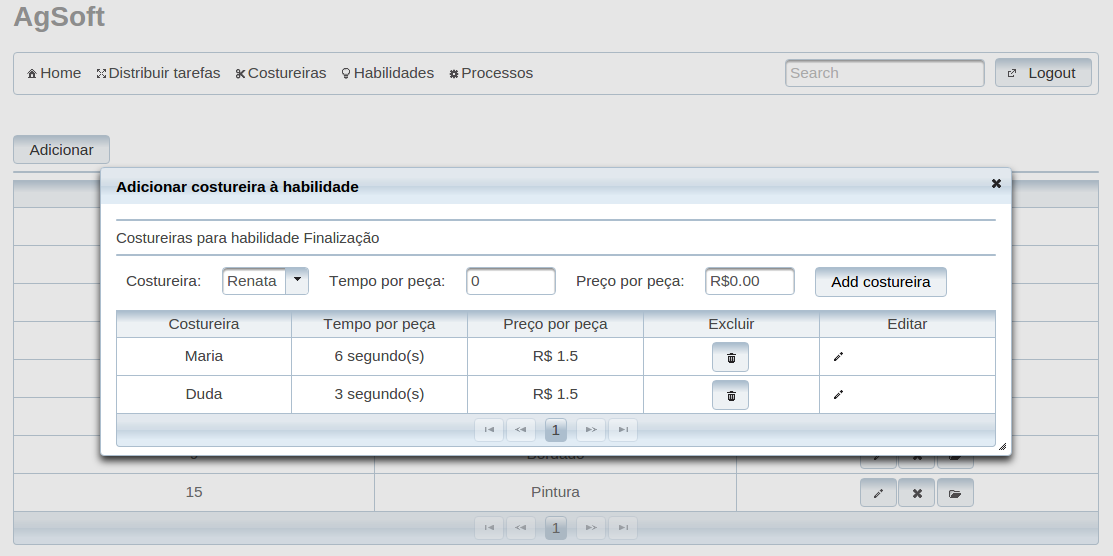
\includegraphics[scale=0.4]{./imagens/tela_habilidade_teste1.png}}
	\caption[Inserindo costureiras na habilidade Finalização.]
	{Inserindo costureiras na habilidade Finalização. \textbf{Fonte:} Desenvolvido
	pelos autores.}
	\label{fig:costureira_habilidade}
\end{figure}


\par Feito isso, foi aberto o processo para a distribuição
das atividades, através do menu "Distribuição de Tarefas".
Ao acessar a página todos os processos criados são
listados como mostra a Figura~\ref{fig:distribuicao_tarefas}:

\begin{figure}[h!]
	\centerline{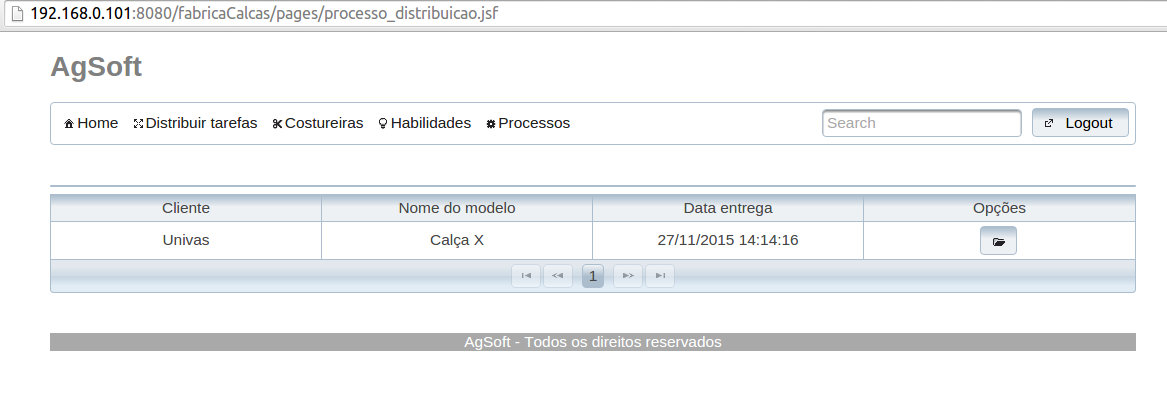
\includegraphics[scale=0.3]{./imagens/tela_distribuicao_tarefas.png}}
	\caption[Tela de distribuição de tarefas.]
	{Tela de dritribuição de tarefas. \textbf{Fonte:} Desenvolvido
	pelos autores.}
	\label{fig:distribuicao_tarefas}
\end{figure}


\par Ao clicar no botão "Abrir" da coluna opções é mostrado a tela para que o
usuário insira os dados, como número de peças, total de peças por lote e data de inicio. Depois de
inseridos os dados, ao clicar no botão "Iniciar Distribuição", o sistema executa
o algoritmo genético e retorna para o usuário a melhor solução
encontrada com base nos dados inseridos, conforme mostra a Figura\ref{fig:resultado_distribuicao_teste1}.

\newpage

\begin{figure}[h!]
	\centerline{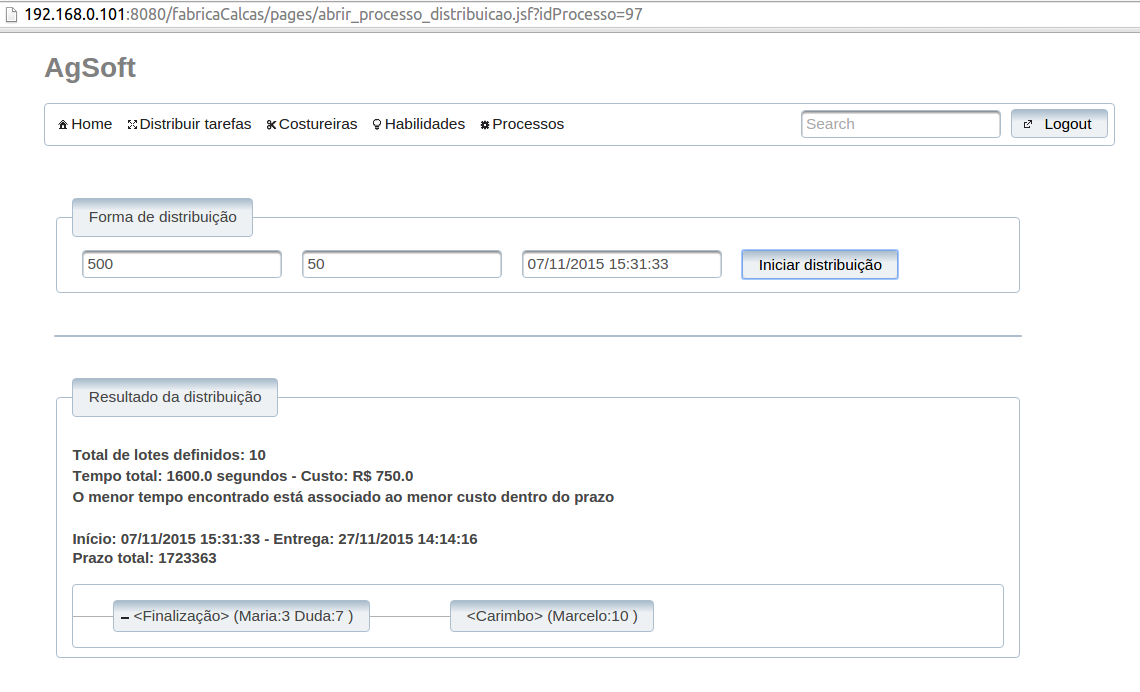
\includegraphics[scale=0.3]{./imagens/resultado_distribuicao_teste1.png}}
	\caption[Resultado da distribuição de lotes.]
	{Resultado da distribuição de lotes. \textbf{Fonte:} Desenvolvido pelos
	autores.}
	\label{fig:resultado_distribuicao_teste1}
\end{figure}

\par Os valores então foram definidos, a distribuição foi realizada, e o resultado apresentado. 
Conforme ilustrado na Figura~\ref{fig:costureira_habilidade}, Maria possui
o tempo de produção maior que Duda, por isso ela recebeu um número menor de lotes
para produzir conforme ilustrado na Figura~\ref{fig:resultado_distribuicao_teste1}

\par Se o tempo de cada costureira for alterado, um novo resultado será
retornado levando em consideração as alterações. Para isto, foi definido para
Maria o tempo de 4 segundos e para Duda o tempo de 7 segundos conforme ilustra a
Figura~\ref{fig:tempo_costureiras}. 



\begin{figure}[h!]
	\centerline{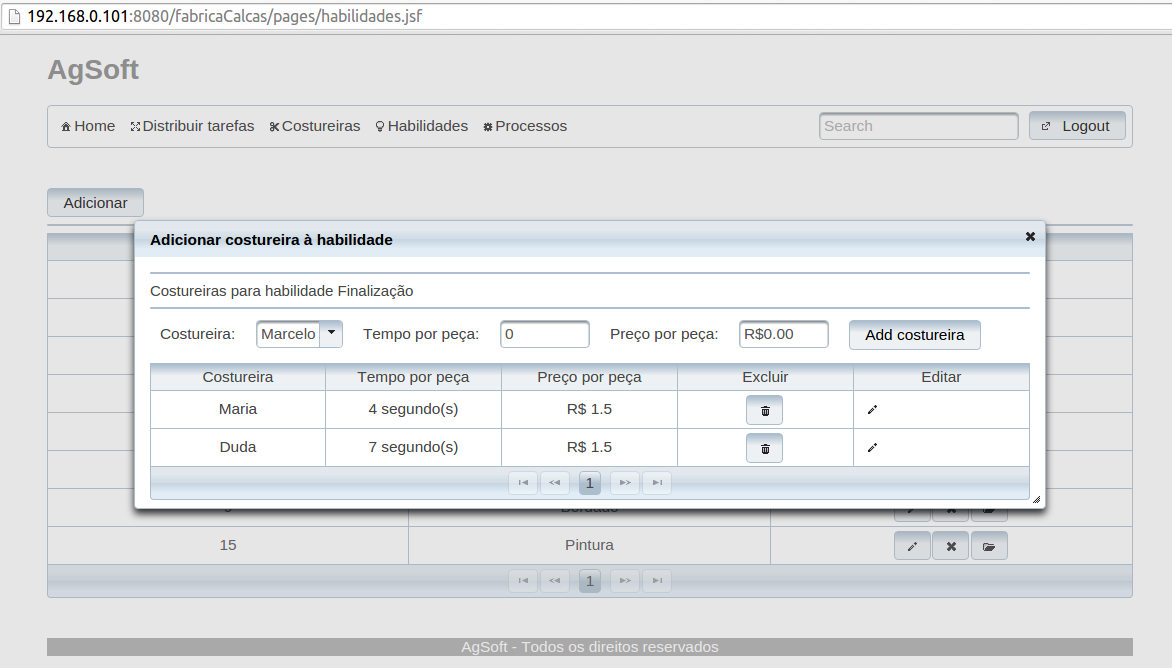
\includegraphics[scale=0.3]{./imagens/alterando_tempo_costureira.png}}
	\caption[Alteração no tempo de produção entre as costureiras.]
	{Alteração no tempo de produção entre as costureiras. \textbf{Fonte:}
	Desenvolvido pelos autores.}
	\label{fig:tempo_costureiras}
\end{figure}

\par Após executar novamente a distribuição foi retornado um novo resultado
ilustrado na Figura~\ref{fig:novo_resultado_distribuicao_teste1}

\newpage

\begin{figure}[h!]
	\centerline{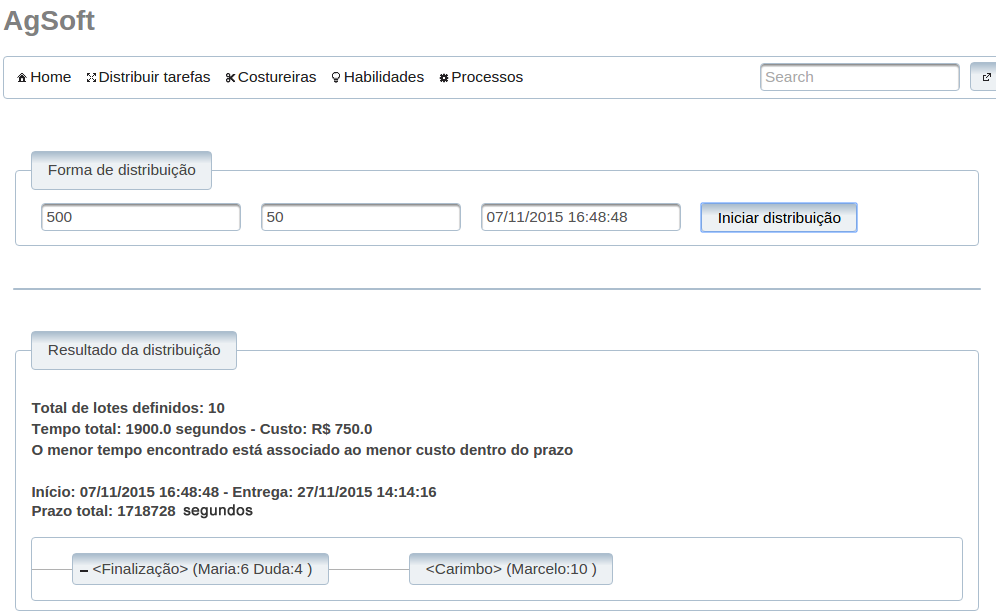
\includegraphics[scale=0.3]{./imagens/novo_resultado_alterado_tempo_teste1.png}}
	\caption[Resultado da distribuição de lotes após a alteração do tempo de
	produção entre as costureiras.]
	{Resultado da distribuição de lotes após a alteração do tempo de
	produção entre as costureiras. \textbf{Fonte:} Desenvolvido pelos autores.}
	\label{fig:novo_resultado_distribuicao_teste1}
\end{figure}

\par Neste resultado Maria obteve mais lotes que Duda para produzir pois o seu tempo de produção é menor.

\section{Teste considerando o custo de produção}

\par Este teste foi feito utilizando-se o mesmo processo do teste realizado na seção anterior,
porém foi definido o mesmo tempo de produção para ambas costureiras alterando somente o custo. Foi definido 
o tempo de 5 segundos para as costureiras Maria e Duda e o preço por peça R\textdollar 1,50 e R\textdollar 
2,70 respectivamente. Além disso foi definido os mesmos valores X e Y relativos a posição geográfica para 
Maria e Duda, de forma a manter o tempo de transporte semelhante para ambas. 
A Figura~\ref{fig:custo_entre_costureiras} mostra a definição de tempo e custo para ambas as costureiras:

\newpage

\begin{figure}[h!]
	\centerline{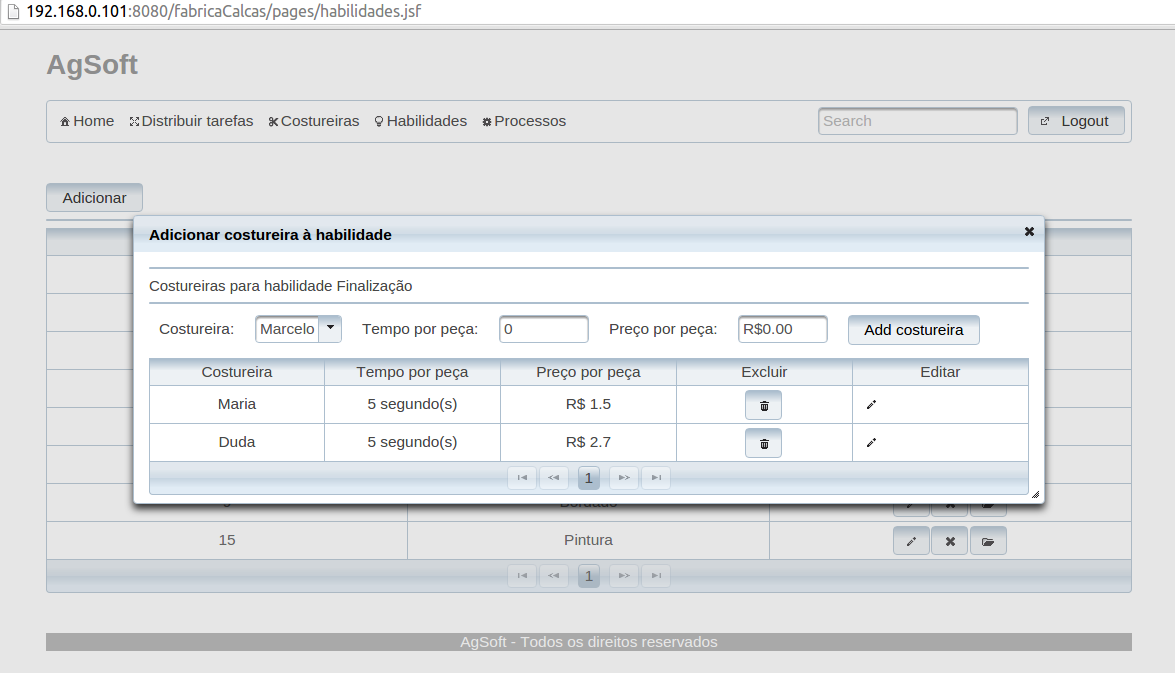
\includegraphics[scale=0.3]{./imagens/custo_entre_costureiras_teste2.png}}
	\caption[Custo entre as costureiras da atividade Finalização.]
	{Custo entre as costureiras da atividade Finalização. \textbf{Fonte:}
	Desenvolvido pelos autores.}
	\label{fig:custo_entre_costureiras}
\end{figure}

\par Ao executar a distribuição é retornado a seguinte resultado ilustrado na Figura~\ref{fig:resultado_custo}:



\begin{figure}[h!]
	\centerline{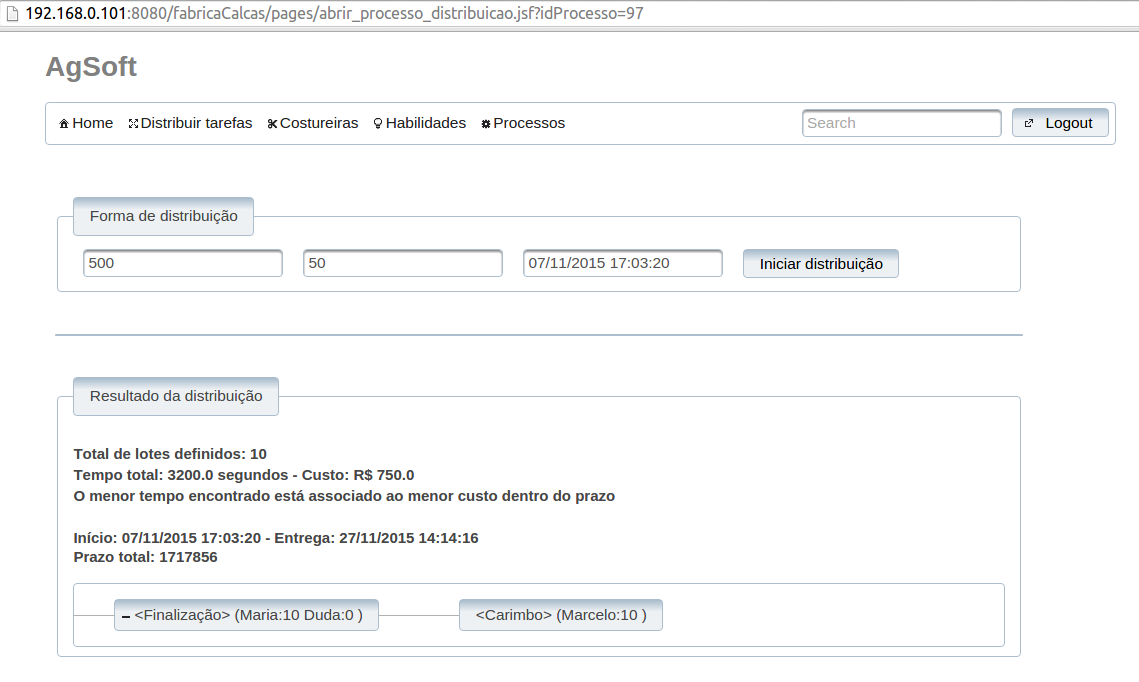
\includegraphics[scale=0.3]{./imagens/resultado_teste2.png}}
	\caption[Resultado da distribuição de lotes considerando o custo.]
	{Resultado da distribuição de lotes considerando o custo. \textbf{Fonte:}
	Desenvolvido pelos autores.}
	\label{fig:resultado_custo}
\end{figure}

\par Com base no resultado obtido, o algoritmo decidiu que, pelo fato de
Maria e Duda obter o mesmo tempo de produção e Duda ter um preço por peça
bem superior que o de Maria, Duda não deve receber nenhum lote para produzir, pois neste
caso é possível que Maria produza sozinha os lotes dentro do prazo de entrega do
processo. Caso Maria não conseguisse produzir os lotes no prazo estipulado, o
algoritmo adequaria a distribuição distribuindo alguns lotes para Duda para
conseguir alcançar o prazo de entrega, toda via, fazendo isto, o custo tende a
aumentar, este caso será mostrado com mais detalhes na seção 4.3.

\par Caso Maria e Duda gastassem o mesmo tempo, cobrassem o mesmo preço e o tempo de
transporte das peças entre todos os envolvidos no processo fosse o mesmo para ambas, 
o algoritmo distribuiria lotes para Duda pois, mesmo a costureira Maria
conseguindo fabricar as peças dentro do prazo, neste caso, se Duda recebesse alguns lotes para produzir
isto não interferiria no preço final e a produção seria realizada em um tempo menor como mostra a Figura~\ref{fig:resultado_tudo_igual}.



\begin{figure}[h!]
	\centerline{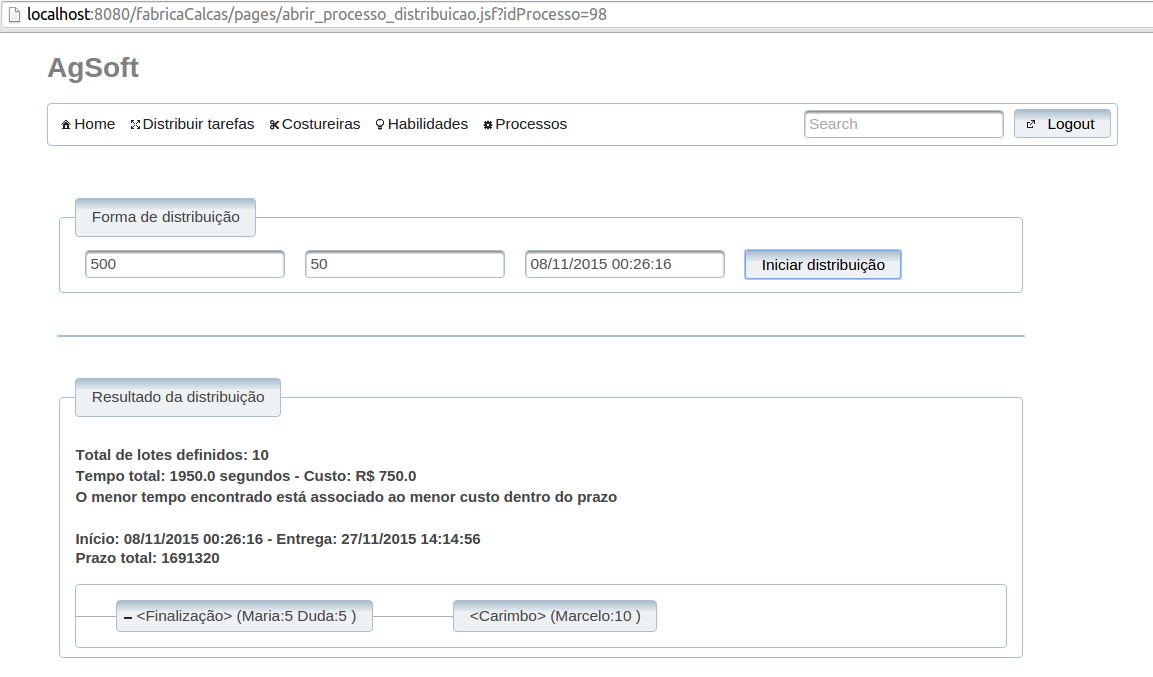
\includegraphics[scale=0.3]{./imagens/resultado_tudo_igual_teste2.png}}
	\caption[Resultado da distribuição de lotes com configurações iguais entre as
	costureiras.] 
	{Resultado da distribuição de lotes com configurações iguais entre as
	costureiras. \textbf{Fonte:}
	Desenvolvido pelos autores.}
	\label{fig:resultado_tudo_igual}
\end{figure}

\section{Teste considerando tempo x custo x prazo de entrega}

\par Este teste foi realizado para demonstrar a distribuição considerando o tempo de
produção, o custo e o prazo de entrega, assim mesmo que uma costureira for inviável 
quanto ao custo, ela poderá receber lotes para produzir para que seja cumprido o prazo 
de entrega. Para isto as costureiras que possuem a habilidade Finalização ficarão com
as seguintes configurações como ilustra a Figura~\ref{fig:configuracao_habilidade_costureira_teste3}.

\newpage

\begin{figure}[h!]
	\centerline{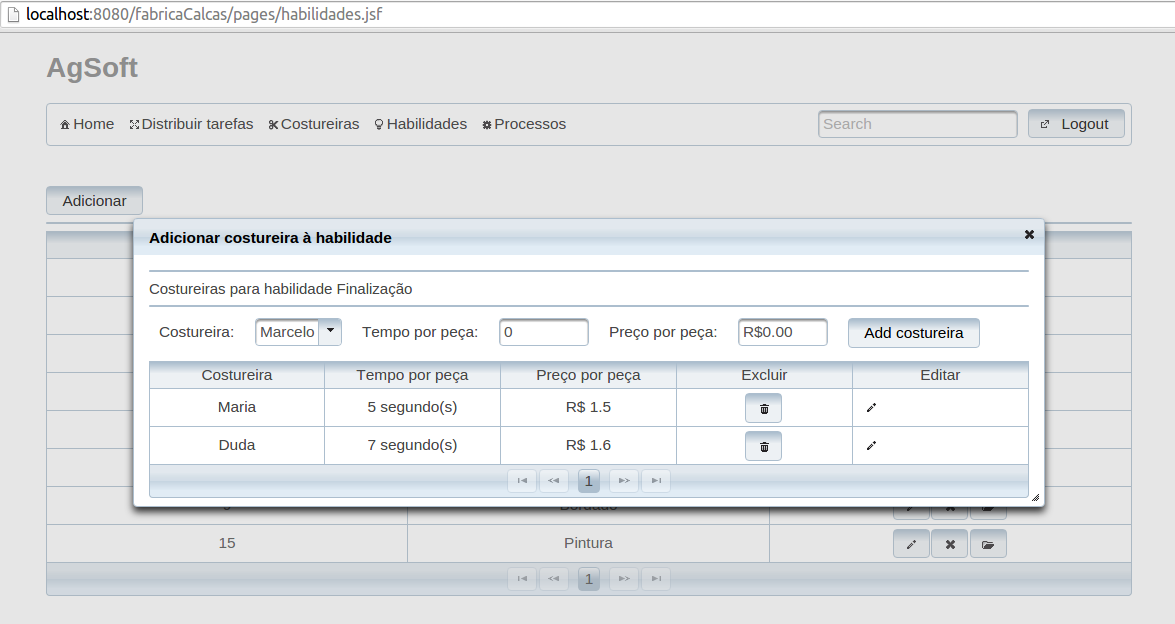
\includegraphics[scale=0.3]{./imagens/cofiguracao_habilidade_teste3.png}}
	\caption[Configuração das costureiras da atividade Finalização.]
	{Configuração das costureiras da atividade Finalização. \textbf{Fonte:}
	Desenvolvido pelos autores.}
	\label{fig:configuracao_habilidade_costureira_teste3}
\end{figure}


\par A Figura~\ref{fig:resultado1_teste3} mostra o resultado da distribuição
com base nas configurações da habilidade Finalização mostrada na Figura~\ref{fig:configuracao_habilidade_costureira_teste3}.

\begin{figure}[h!]
	\centerline{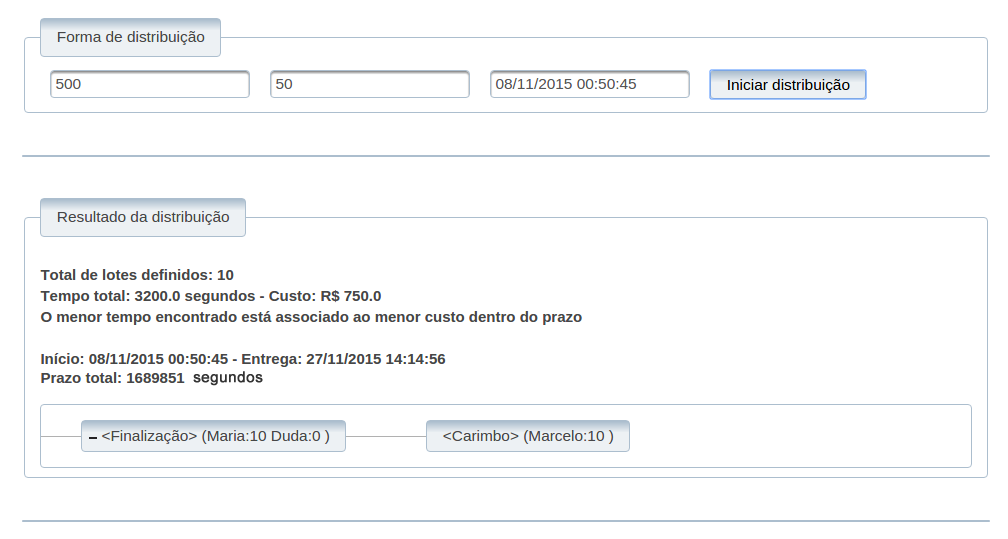
\includegraphics[scale=0.3]{./imagens/resultado1_teste3.png}}
	\caption[Resultado da distribuição de lotes com prazo longo.]
	{Resultado da distribuição de lotes com prazo longo. \textbf{Fonte:} Desenvolvido pelos
	autores.}
	\label{fig:resultado1_teste3}
\end{figure}

\par Como ilustrado na Figura~\ref{fig:resultado1_teste3}, a costureira Duda
não recebeu nenhum lote pois possui um tempo de produção e custo maior que Maria e
esta consegue cumprir o prazo de entrega, porém, caso Maria não conseguisse atender
o prazo, Duda poderia receber lotes para produzir mesmo que custo aumente.

A Figura~\ref{fig:resultado2_teste3} mostra a distribuição de lotes entre as
costureiras com a alteração na data de início do processo.

\newpage

\begin{figure}[h!]
	\centerline{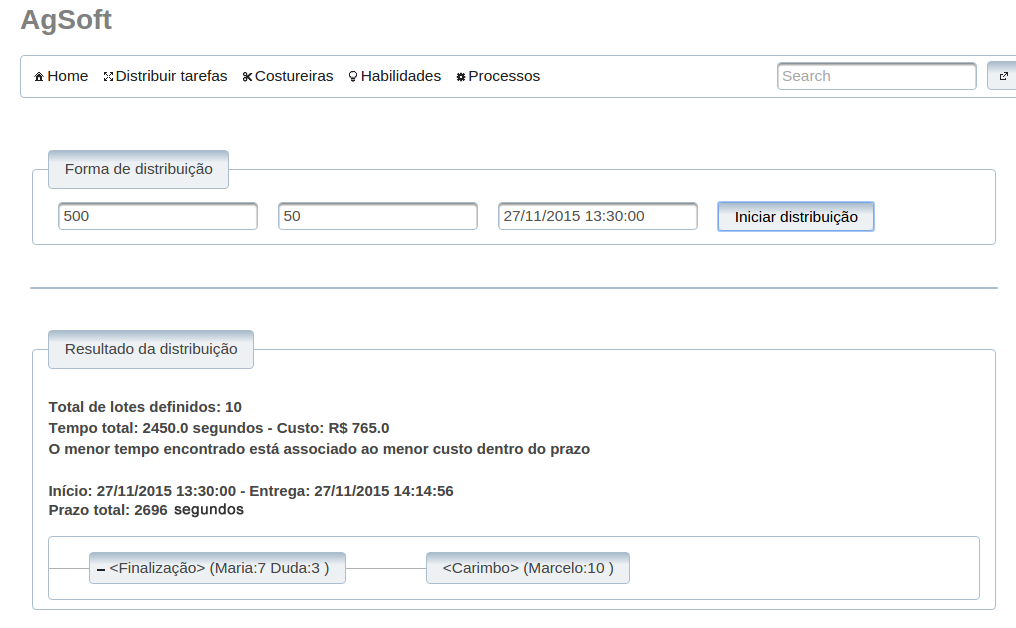
\includegraphics[scale=0.3]{./imagens/resultado2_teste3.png}}
	\caption[Resultado da distribuição de lotes com prazo reduzido.]
	{Resultado da distribuição de lotes com prazo reduzido. \textbf{Fonte:} Desenvolvido pelos
	autores.}
	\label{fig:resultado2_teste3}
\end{figure}

\par Como ilustrado na Figura~\ref{fig:resultado2_teste3} a costureira Duda
recebe 3 lotes para produzir, assim, o custo de produção aumenta com relação ao 
resultado da Figura~\ref{fig:resultado1_teste3}, porém o tempo de produção diminui
sendo possível atender o prazo de entrega.


\section{Teste considerando o tempo de transporte}

\par Este teste foi realizado para demonstrar que mesmo as costureiras possuindo
o tempo e custo iguais, o tempo de transporte entre elas pode influenciar na distribuição dos lotes.

\par Para isto, foi necessário cadastrar um valor X e Y para cada costureira, 
conforme mostra a Figura~\ref{fig:add_xy_costureira_teste4}.




\begin{figure}[h!]
	\centerline{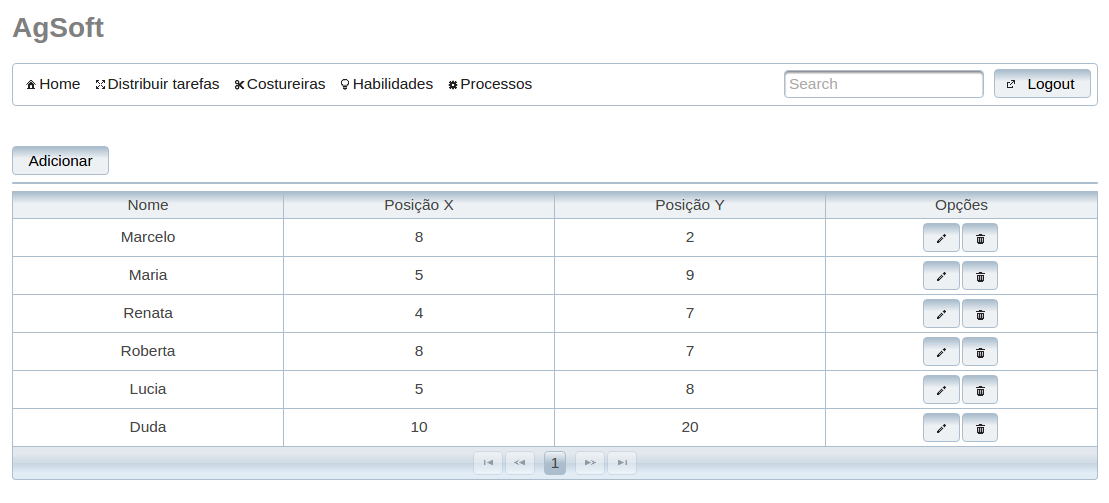
\includegraphics[scale=0.3]{./imagens/posicao_xy_costureiras_teste4.png}}
	\caption[Tela de cadastro de costureiras.]
	{Tela de cadastro de costureiras. \textbf{Fonte:} Desenvolvido pelos autores.}
	\label{fig:add_xy_costureira_teste4}
\end{figure}



\par Neste teste foi considerado apenas o tempo de transporte, logo o tempo de
confecção por peça das costureiras da atividade Finalização possuem o mesmo
valor de tempo e custo, conforme mostra a Figura~\ref{fig:at_finalizacao_teste4}.


\begin{figure}[h!]
	\centerline{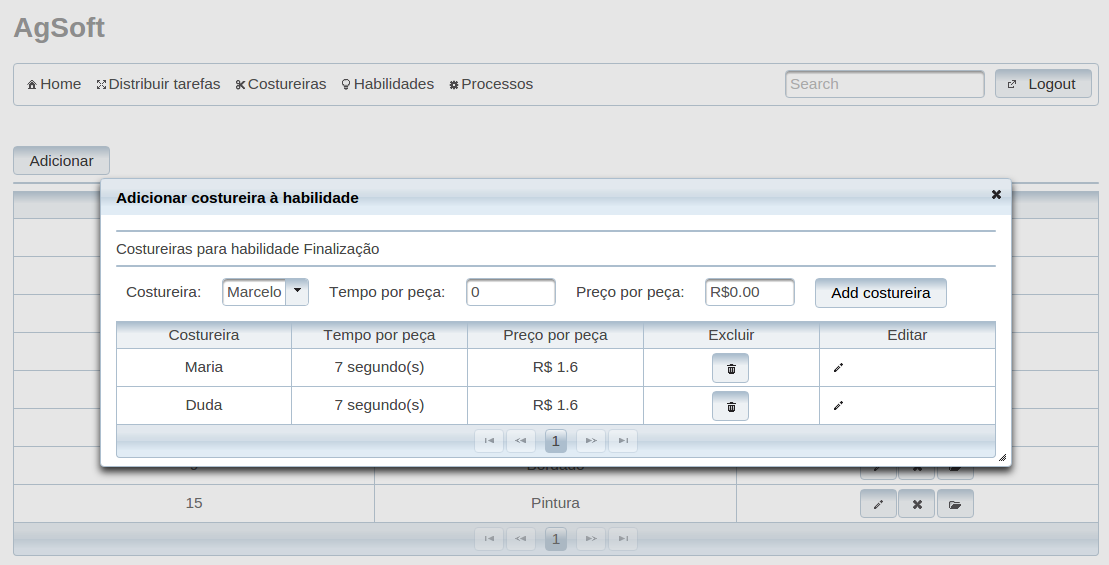
\includegraphics[scale=0.3]{./imagens/cofig_at_finalizaca_teste4.png}}
	\caption[Configuração das costureiras da habilidade Finalização.]
	{Configuração das costureiras da habilidade Finalização \textbf{Fonte:}
	Desenvolvido pelos autores.}
	\label{fig:at_finalizacao_teste4}
\end{figure}



\par Feito isto, foi iniciado então o processo de distribuição das atividades,
através do menu Distribuição de Tarefas, a Figura~\ref{fig:resultado_transporte_teste4} mostra o resultado obtido.


\begin{figure}[h!]
	\centerline{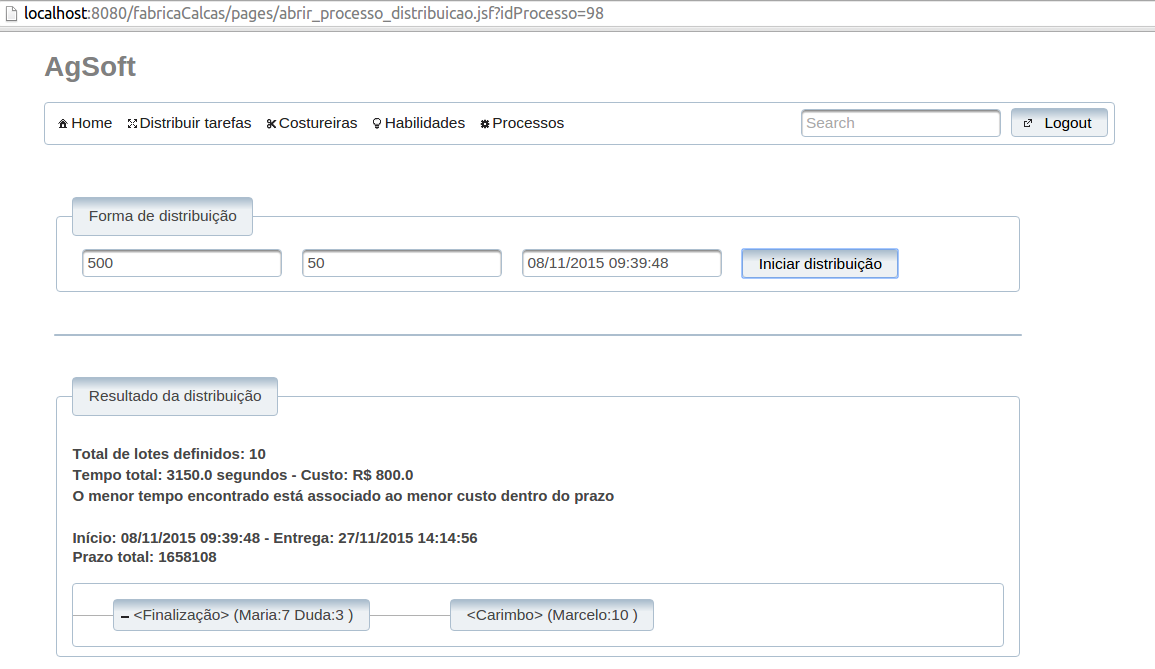
\includegraphics[scale=0.3]{./imagens/resultado_transporte_teste4.png}}
	\caption[Resultado da disttribuição de lotes.]
	{Resultado da disttribuição de lotes. \textbf{Fonte:} Desenvolvido pelos
	autores.}
	\label{fig:resultado_transporte_teste4}
\end{figure}

\par Como mostrado na Figura~\ref{fig:add_xy_costureira_teste4}, a costureira
Duda fica mais distante do Marcelo e por isso recebe menos lotes para produzir em
relação a costureira Maria.

\par Para melhor ilustrar o tempo de envio das peças para as costureiras, na tela
de resultados há um detalhamento de todo calculo realizado, a Figura~\ref{fig:detalhameneto_transporte_teste4} 
mostra que o tempo de envio da peças para Duda é 
maior que o tempo de envio para Maria, comprovando o resultado mostrado na
Figura~\ref{fig:resultado_transporte_teste4}.

\begin{figure}[h!]
	\centerline{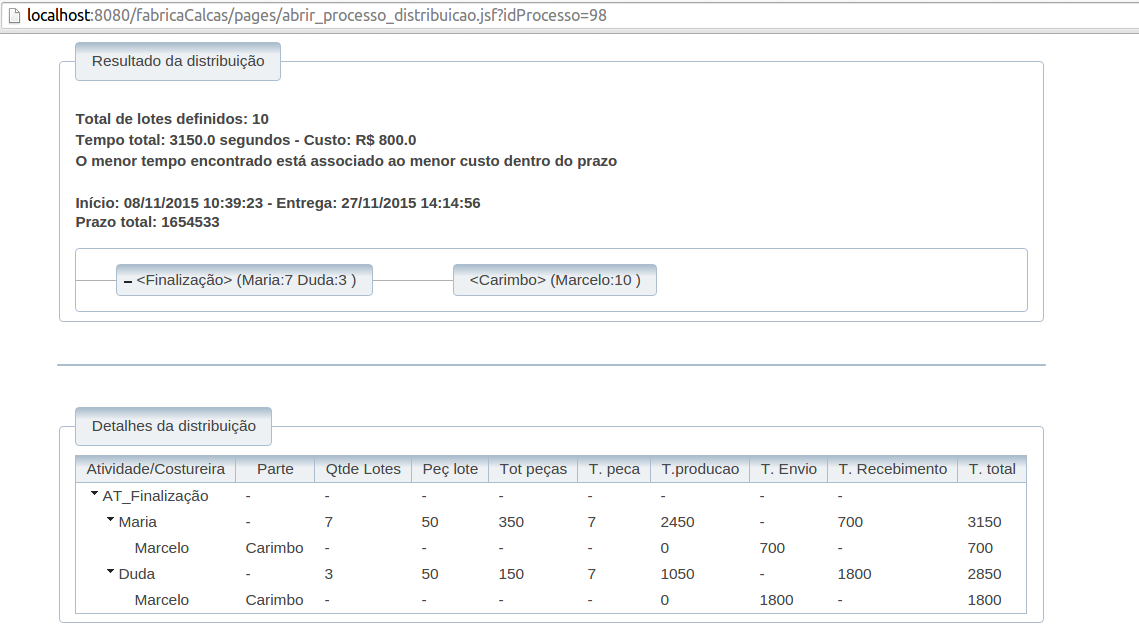
\includegraphics[scale=0.3]{./imagens/detalhamento_transporte_teste4.png}}
	\caption[Distribuição das atividades.] 
	{Distribuição das atividades. \textbf{Fonte:} Desenvolvido pelos autores.}
	\label{fig:detalhameneto_transporte_teste4}
\end{figure}

\par Como mostrado na Figura~\ref{fig:detalhameneto_transporte_teste4}, o tempo
de envio das peças para Duda é 1800 segundos e para Maria 700, por isso
Duda recebe menos lotes para ser produzidos.


\section{Teste adicionando mais atividades ao processo}

\par Este teste foi realizado para demonstrar a adição de mais atividades no
processo. Este teste segue o mesmo processo da seção 4.1.

\par Neste caso deve-se considerar o tempo de transporte entre as costureiras da atividade Frente e o Marcelo 
para a retirada dos materiais e o tempo entre tais costureiras e a costureira
responsável pela Finalização, para isso foi adicionado no processo a atividade
Frente conforme mostra a Figura~\ref{fig:add_frente_teste5}.

\newpage

\begin{figure}[h!]
	\centerline{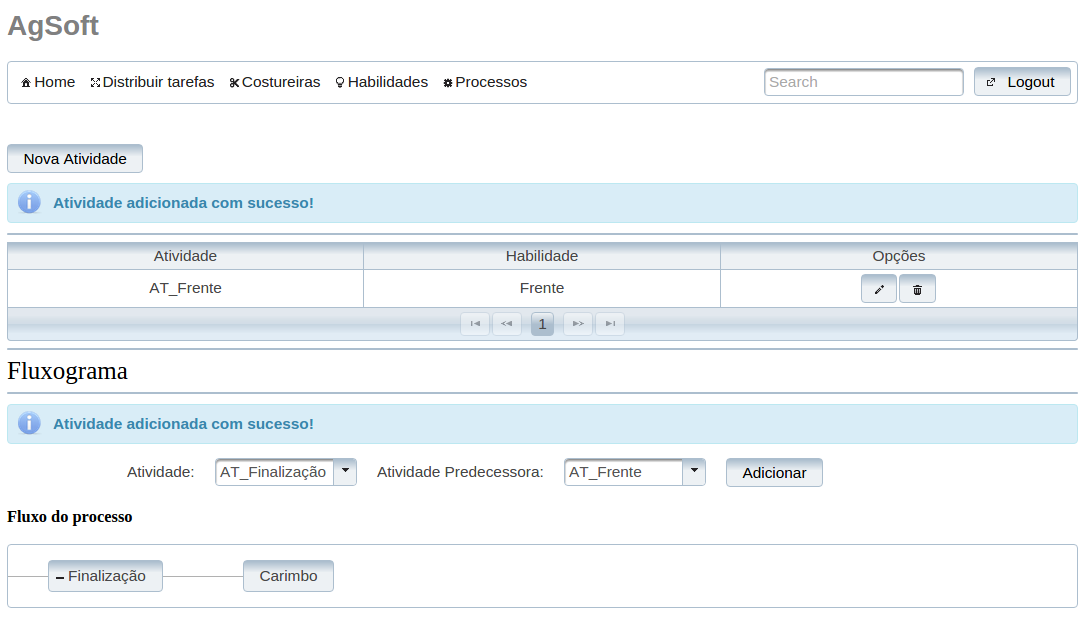
\includegraphics[scale=0.3]{./imagens/adiconar_atividade_frente_teste5.png}}
	\caption[Adição de uma atividade ao processo.]
	{Adição de uma atividade ao processo. \textbf{Fonte:} Desenvolvido pelos
	autores.}
	\label{fig:add_frente_teste5}
\end{figure}

\par Após a adição da atividade, é preciso adicioná-la ao fluxo do processo como
predecessora da atividade Finalização. Como a atividade Finalização é sempre a
última atividade do processo, todas as atividades que forem incluídas sempre
serão predecessoras a ela. A Figura~\ref{fig:add_frente_teste4} mostra a atividade Frente adicionada
no fluxo do processo.



\begin{figure}[h!]
	\centerline{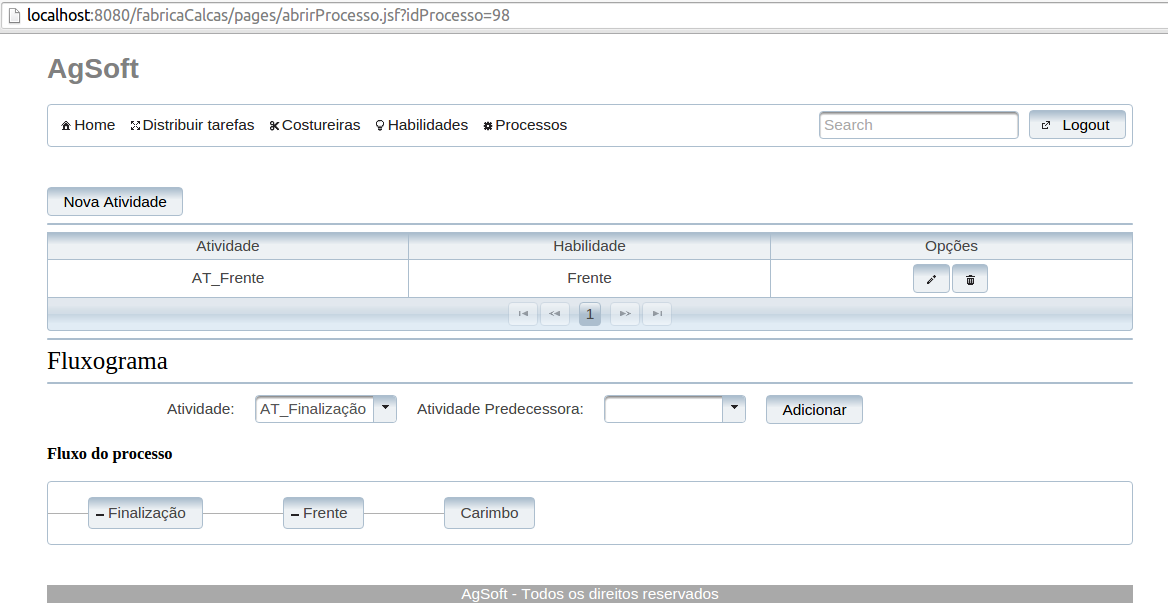
\includegraphics[scale=0.3]{./imagens/adicionar_atividade_frente_teste4.png}}
	\caption[Adição de uma atividade ao fluxo do processo.]
	{Adição de uma atividade ao fluxo do processo. \textbf{Fonte:} Desenvolvido
	pelos autores.}
	\label{fig:add_frente_teste4}
\end{figure}


\par Foi adicionado na habilidade Frente as costureiras Roberta, Lúcia e Renata
para que estas possam realizar a atividade Frente do processo.
\par A Figura~\ref{fig:add_costureira_frente_teste4} mostra as costureiras
adicionadas na habilidade Frente.

\newpage

\begin{figure}[h!]
	\centerline{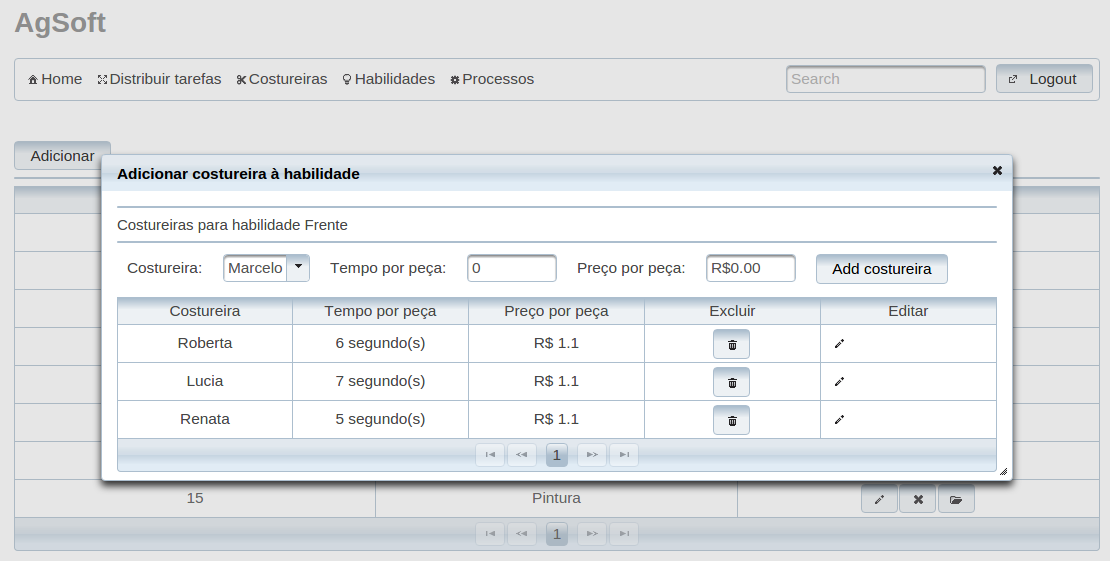
\includegraphics[scale=0.3]{./imagens/costureiras_at_frente_tete5.png}}
	\caption[Adição de costureiras na habilidade Frente.]
	{Adição de costureiras na habilidade Frente. \textbf{Fonte:} Desenvolvido pelos
	autores.}
	\label{fig:add_costureira_frente_teste4}
\end{figure}

\par Feito isso foi realizado a distribuição dos lotes com as configurações de
tempo e custo mostradas na Figura~\ref{fig:add_costureira_frente_teste4} e com
as configurações de posicionamento mostradas na Figura~\ref{fig:add_xy_costureira_teste4}.
\par A Figura~\ref{fig:resultado1_teste5} mostra o resultado obtido na
distribuição.



\begin{figure}[h!]
	\centerline{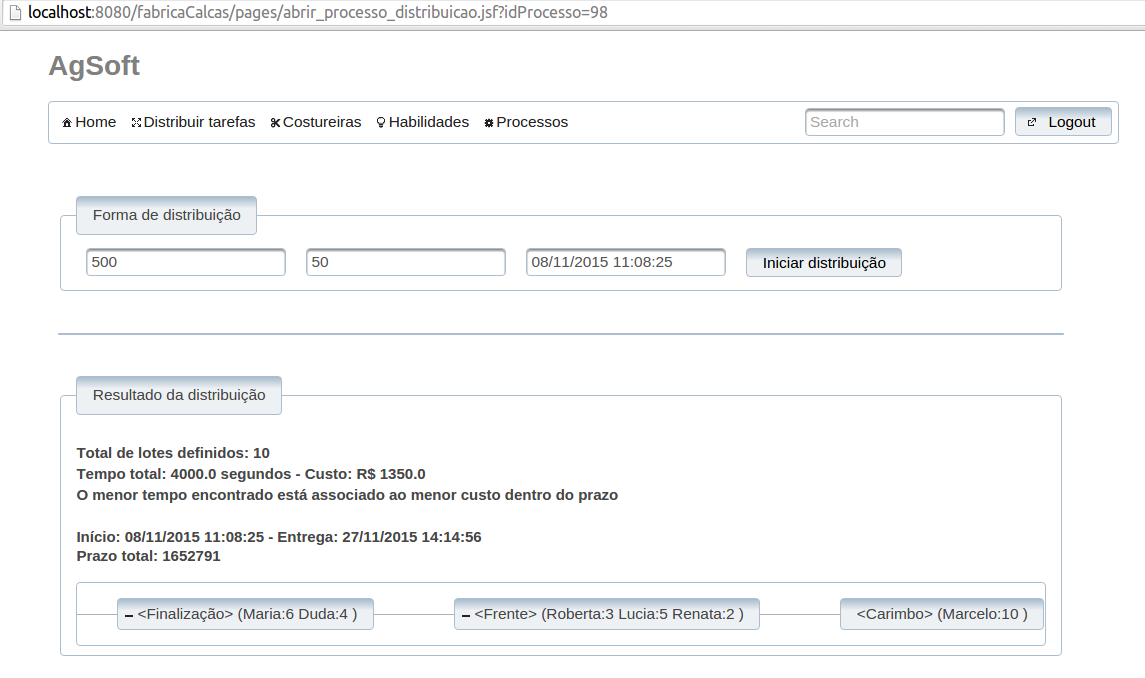
\includegraphics[scale=0.3]{./imagens/resultado1_teste5.png}}
	\caption[Resultado da distribuição de lotes.]
	{Resultado da distribuição de lotes. \textbf{Fonte:} Desenvolvido pelos
	autores.}
	\label{fig:resultado1_teste5}
\end{figure}

\par Com base na Figura~\ref{fig:resultado1_teste5} pode-se observar que foi
adicionado no resultado final a atividade Frente e suas respectivas costureiras.

\par A Figura~\ref{fig:detalhamento1_teste5} mostra o detalhamento da
distribuição da Figura~\ref{fig:resultado1_teste5}.

\newpage

\begin{figure}[h!]
	\centerline{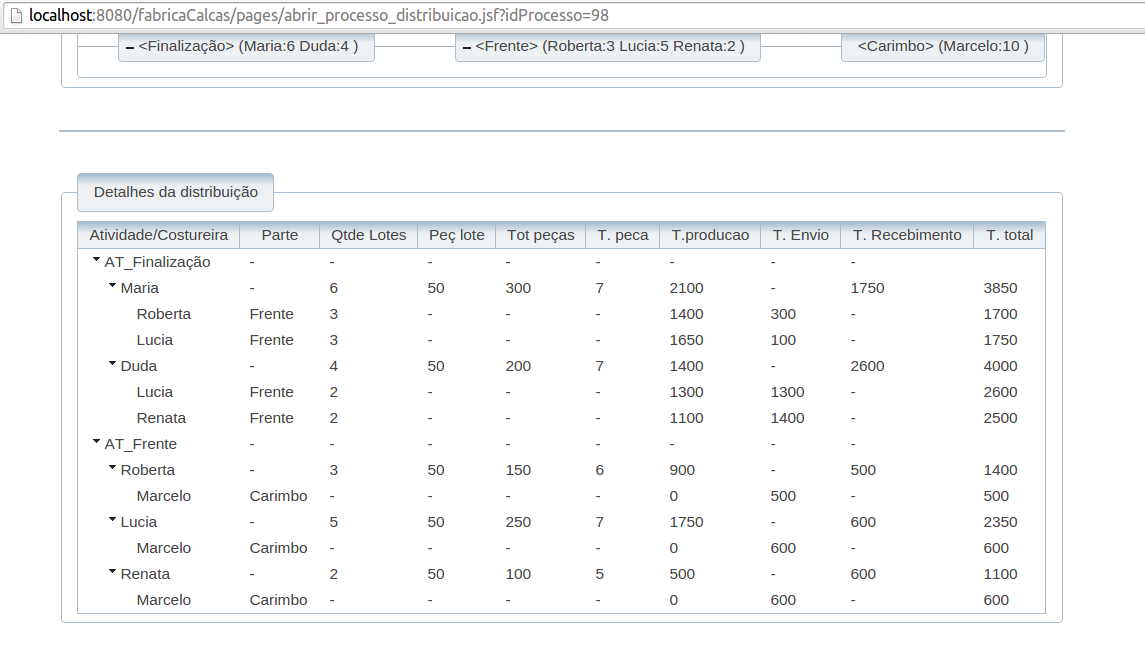
\includegraphics[scale=0.3]{./imagens/detalhamento1_teste5.png}}
	\caption[Distribuição das atividades.]
	{Distribuição das atividades. \textbf{Fonte:} Desenvolvido pelos
	autores.}
	\label{fig:detalhamento1_teste5}
\end{figure}

\par Vale ressaltar que ao executar a distribuição o algoritmo pode
encontrar várias soluções que contém o mesmo resultado e retorna uma delas, se a
distribuição for executada novamente mantendo as configurações das costureiras
como a posição X e Y, tempo e custo, a distribuição poderá ocorrer de uma outra
forma conforme mostra a Figura~\ref{fig:resultado2_teste5}.



\begin{figure}[h!]
	\centerline{\includegraphics[scale=0.3]{./imagens/resultado2_teste5.png}}
	\caption[Resultado da distribuição de lotes após executar novamente a
	distribuição.]
	{Resultado da distribuição de lotes após executar novamente a
	distribuição. \textbf{Fonte:} Desenvolvido pelos autores.}
	\label{fig:resultado2_teste5}
\end{figure}


\par A Figura~\ref{fig:detalhamento2_teste5} mostra o detalhamento da
distribuição da Figura~\ref{fig:resultado2_teste5}.

\newpage

\begin{figure}[h!]
	\centerline{\includegraphics[scale=0.3]{./imagens/detalhamento2_teste5.png}}
	\caption[Distribuição das atividades.] 
	{Distribuição das atividades. \textbf{Fonte:} Desenvolvido pelos
	autores.}
	\label{fig:detalhamento2_teste5}
\end{figure}


\par Com base nas Figuras~\ref{fig:resultado1_teste5} e~\ref{fig:resultado2_teste5}
o custo final não teve alterações de uma distribuição para outra, porém 
pode-se observar que o tempo total de produção e o
distribuição dos lotes entre as costureiras é realizado de uma forma
diferente, concluindo assim que o algoritmo encontrou outra forma de realizar a
distribuição mantendo o melhor resultado.

\section{Teste quando o prazo não é atendido}

\par Este teste foi realizado para demonstrar quando o prazo de entrega das
peças não consegue ser atendido. Este teste segue o mesmo processo da seção 4.1.

\par A Figura~\ref{fig:configuracao_costureiras_teste6} mostra a configuração
das costureiras da habilidade finalização.

\begin{figure}[h!]
	\centerline{\includegraphics[scale=0.3]{./imagens/configuracao_costureiras_teste6.png}}
	\caption[Configuração das costureiras da atividade Finalização.] 
	{Configuração das costureiras da atividade Finalização. \textbf{Fonte:} Desenvolvido pelos
	autores.}
	\label{fig:configuracao_costureiras_teste6}
\end{figure}

\par Considerando as configurações mostradas na Figura~\ref{fig:configuracao_costureiras_teste6} foi iniciado o processo de
distribuição dos lotes como mostra a Figura~\ref{fig:resultado1_teste6}.

\begin{figure}[h!]
	\centerline{\includegraphics[scale=0.3]{./imagens/resultado1_teste6.png}}
	\caption[Resultado da distribuição de lotes.] 
	{Resultado da distribuição de lotes. \textbf{Fonte:} Desenvolvido pelos
	autores.}
	\label{fig:resultado1_teste6}
\end{figure}

\par Como mostrado na Figura~\ref{fig:resultado1_teste6}, o prazo de produção
é de 1796 segundos e, mesmo alocando todas as costureiras não foi possível
entregar as peças no prazo determinado pois o tempo mínimo possível de produção
é de 2450 segundos. O algoritmo foi desenvolvido para manter sempre o menor custo, procurando manter o tempo
dentro do prazo, porém caso nenhum dos indivíduos tenham o tempo total menor que o prazo,
então o melhor tempo é retornado e a ordenação por custo é ignorada. Para
demonstrar isto, foi alterado o custo da costureira Duda conforme mostra a Figura~\ref{fig:alterecao_custotcseis}.
 

\begin{figure}[h!]
	\centerline{\includegraphics[scale=0.3]{./imagens/alterecao_custo_teste6.png}}
	\caption[Alteração no custo das costureiras da habilidade Finalização.] 
	{Resultado da distribuição após alteração no custo da costureira Duda. \textbf{Fonte:} Desenvolvido pelos
		autores.}
	\label{fig:alterecao_custotcseis}
\end{figure}

\par Foi iniciado novamente a distribuição dos lotes conforme mostra a Figura~\ref{fig:resultado2_teste6}.

\begin{figure}[h!]
	\centerline{\includegraphics[scale=0.3]{./imagens/resultado2_teste6.png}}
	\caption[Resultado da distribuição após alteração no custo da costureira Duda.] 
	{Resultado da distribuição após alteração no custo da costureira Duda. \textbf{Fonte:} Desenvolvido pelos
	autores.}
	\label{fig:resultado2_teste6}
\end{figure}

\par Conforme mostrado na Figura~\ref{fig:resultado2_teste6}, mesmo com o
aumento no custo por peça da costureira Duda, o algoritmo mesmo assim distribuiu
lotes para esta costureira aumentando o custo final porém retornou o
menor tempo de produção possível.

%
\chapter{CONCLUSÃO} 

\par A conclusão deste trabalho é \ldots

\par Assim conclui-se que\ldots




\postextual %Início dos Elementos Pós-Textuais

%\citeoption{abnt-etal-cite=2}
\citeoption{ABNT-final}

%\bibliography{nuapatex-options, biblio}			            % insere as REFERENCIAS
\bibliography{biblio}			            % insere as REFERENCIAS (arquivo biblio.bib)
\addcontentsline{toc}{chapter}{REFERÊNCIAS} % adiciona o título no sumário

%\begin{apendicesenv}

%\apendicesname{APÊNDICES}
% Imprime uma página indicando o início dos apêndices
\partapendices*

\addcontentsline{toc}{chapter}{APÊNDICES}

\chapter*{Título do Apêndice I}
\label{apendice:1}

\par Aqui deve conter o texto do Apêndice~\ref{apendice:1}. Na Figura~\ref{fig:ap1:identificador} é ilustrada a primeira tela deste processo.
\captionsetup[figure]{list=no}
\begin{figure}[h!]
 \centerline{\includegraphics[scale=0.5]{./imagens/apendice_img1.png}}
 \caption[Outra imagem.]
           {Outra imagem. \textbf{Fonte:} Elaborado pelos autores}
  \label{fig:ap1:identificador}
\end{figure}

\par Após a seleção do tipo de projeto \ldots
\chapter*{Título do Apêndice 2}

\section*{Primeira seção do apêndice 2}

\par Neste apêndice é mostrado \ldots de acordo com a Figura~\ref{fig:ap2:identificador} é ilustrada a primeira tela deste processo.
\captionsetup[figure]{list=no}
\begin{figure}[h!]
 \centerline{\includegraphics[scale=0.3]{./imagens/apendice_img1.png}}
 \caption[Outra imagem ainda.]
           {Outra imagem ainda. \textbf{Fonte:} Elaborado pelos autores}
  \label{fig:ap2:identificador}
\end{figure}

\section*{Segunda seção do apêndice 2}


\par Continuando \ldots na figura Figura~\ref{fig:xml_exemplo} é mostrado um exemplo de XML.

\begin{figure}[h!]
\begin{lstlisting}[style=custom_XML]
<project>
...
 <dependencies>
  ...
  <dependency>
   <groupId>org.neo4j</groupId>
   <artifactId>neo4j</artifactId>
   <version>1.9.4</version>
  </dependency>
  ...
 </dependencies>
 ...
</project>
\end{lstlisting}  
 \caption[Exemplo de código XML.]
           {Exemplo de código XML. \textbf{Fonte:} Elaborado pelos autores}
  \label{fig:xml_exemplo}
\end{figure}



\end{apendicesenv}
%%\anexoname{ANEXOS}
%\begin{anexosenv}
%\partanexos
%\chapter*{ANEXO I}

%\end{anexosenv}

\addcontentsline{toc}{chapter}{ANEXOS}

\chapter*{ANEXO I}



\printindex

\end{document}